% !TeX spellcheck = en_GB
%\documentclass[11pt,DIV=11,a4paper,BCOR=15mm,twoside=on,bibliography=leveldown]{scrbook}
%\documentclass[11pt,DIV=11,a4paper,BCOR=15mm]{scrbook}
\documentclass[%
  11pt,
  DIV=16,
  a4paper,
  BCOR=15mm,
  twoside=on,
  bibliography=totoc,
  headings=normal,
  titlepage,
  numbers=noendperiod,
  appendixprefix=true
%  captions=tableheading,
%  chapterprefix=true% like in standard class "report"
]{scrreprt}
%\documentclass[11pt,DIV=11,a4paper]{scrartcl}
\usepackage[sign]{ma} % Options: sign, print

\title{Modelling and Automated Retrieval of Provenance Relationships}
\author{Thomas Schneider}

\begin{document}

  \pagenumbering{roman}
  % \maketitle
  \selectlanguage{ngerman}
  % !TeX spellcheck = de_DE
\thispagestyle{plain}
\begin{titlepage}

  \begin{center}
  
    \vspace*{1cm}
    Humboldt-Universität zu Berlin \\
    Philosophische Fakultät \\
    Institut für Bibliotheks- und Informationswissenschaft
  
    \vspace*{\fill}
    {\Huge\bfseries\sffamily
      Modelling and Automated Retrieval \\[6pt]
      of Provenance Relationships
    }
    
    \vspace*{\fill}
    Masterarbeit im Rahmen des Weiterbildenden Masterstudiengangs\\
    Bibliotheks- und Informationswissenschaft im Fernstudium
    
    \vspace*{\fill}
    vorgelegt von \\
    Thomas Schneider
    
    \vspace*{\fill}
    Gutachter: \\
    Prof.\ Dr.\ Robert Jäschke \\
    Christian Rüter
    
    \vspace*{\fill}
    Erfurt, den \today
    
    \vspace*{1cm}
    
%    \copyright\ 2023\\[9ex]
  
  \end{center}
  
%%  \singlespacing
%  \small
%  \noindent Dieses Werk einschließlich seiner Teile ist \textbf{urheberrechtlich geschützt}. Jede Verwertung außerhalb der engen Grenzen des Urheberrechtgesetzes ist ohne Zustimmung des Autors unzulässig und strafbar. Das gilt insbesondere für Vervielfältigungen, Übersetzungen, Mikroverfilmungen sowie die Einspeicherung und Verarbeitung in elektronischen Systemen.

\end{titlepage}
%  \setcounter{tocdepth}{1} % include only chapters and sections in table of contents
%  \setcounter{tocdepth}{2} % include only chapters, sections, and subsections in table of contents
  \selectlanguage{UKenglish}
  \clearpage
%  \listoftodos
%  \clearpage
  \tableofcontents
  \clearpage
  \listoffigures
  

%  \clearpage
%  % !TeX spellcheck = en_GB
% =================================================================
\chapter*{Sketchbook}

% -------------------------------------------------------------------
\section*{``Storyline''}

\begin{tikzpicture}[
  >=Latex,
  every node/.style={draw=none,fill=none,thick,inner sep=1.5mm},
  every edge/.style={draw=black,thick}  
]
  \node                                 (queries)         {Prototype queries};
  \node [below=10mm of queries]         (datasources)     {\tikztab[c]{Requirement analysis:\\[-1pt]Analysis of available data sources\\[-1pt]Analysis of possible queries}};
  \node [below=10mm of datasources]     (modelling)       {Modelling};
  \node [below=10mm of modelling]       (dataintegration) {Data integration};
  \node [below=10mm of dataintegration] (method)          {Method};
  
  \path[->]
    (queries)         edge (datasources)
    (datasources)     edge (modelling)
    (modelling)       edge (dataintegration)
    (dataintegration) edge (method)
  ;
  
\end{tikzpicture}

\begin{itemize}
  \item 
    Modelling depends on requirement analysis: why is it appropriate to use graphs rather than ``fully-fledged'' database theory?
  \item
    OTOH, the early specification of prototype queries will necessarily remain vague and extensional
    as long as we don't have an abstract model!
  \item
    perhaps use ``lightweight'' def. of a conjunctive query?
\end{itemize}


%
  \clearpage
  \pagestyle{headings}
  \pagenumbering{arabic}
  % !TeX spellcheck = en_GB
% =================================================================
\chapter{Introduction}
\label{chap:intro}

% -----------------------------------------------------------------
\section{Setting}
\label{sec:setting}

In research on the historical holdings of university and research libraries,
the origins of book copies\todo{really restrict to books?} are of central importance.
The origin of an item is also called its \emph{provenance} 
and comprises the people or corporations that owned this item over time.
Particularly interesting provenances are those related to the change of
owners when book copies are passed on or distributed \autocite[p.\,2]{Hakelberg2016}.
Provenances can be reconstructed by marks of ownership
such as stamps, bookplates (ex libris), or handwritten signatures:
with the help of these features, it is possible to retrace
the ``history'' of a book copy
or the extent of library holdings that have been scattered in the meantime \autocite[p.\,2]{Hakelberg2016}.

In order to enable provenance research,
libraries index the provenances of their historical holdings
and make them available to users via their catalogues.
A provenance entry refers to a person or corporation
and to a feature that indicates ownership.
In order for owners to be identified unequivocally,
they are often given via a reference to authority files such as the
Integrated Authority File (GND) of the German National Library.%
\footnote{%
  \url{https://www.dnb.de/EN/Professionell/Standardisierung/GND/gnd.html}%
}
The indexed provenance data makes it possible, for example,
to query and reconstruct the books owned or held by a single person or corporation,
to query the whereabouts of relevant copies,
or to retrace the distribution of all indexed copies of a work.

In the digital age, provenance entries are recorded in electronic catalogues.
German university and research libraries typically do not 
maintain their own individual catalogue; rather they are provided with a central
catalogue by the library network in which they participate.%
\footnote{%
  There are six library networks \emph{(Bibliotheksverbünde)} for scientific libraries
  in Germany: \url{https://de.wikipedia.org/wiki/Bibliotheksverbund\#Deutschland}%
}
These central catalogues are equipped with an underlying database
and standardised data formats for internal representation and data export.
For example, the networks GBV and SWB maintain and use the common catalogue (database)
\emph{K10plus},%
\footnote{\url{https://www.bszgbv.de/services/k10plus/}}
which internally uses the data format PICA%
\footnote{\url{https://format.gbv.de/pica}}
and allows for exports in the data formats
MARC 21, MAB2, and Pica+.%
\footnote{\url{https://wiki.k10plus.de/display/K10PLUS/Exportformate}}
%  \footnote{\url{https://de.wikipedia.org/wiki/Machine-Readable_Cataloging}}%
%  \footnote{\url{https://www.dnb.de/DE/Professionell/Metadatendienste/Exportformate/MARC21/marc21_node.html}}
Despite the use of a uniform data format,
there are several possibilities to record provenance entries.
As Hakelberg \autocite*[Chapter~4]{Hakelberg2016} explains,
libraries even within the same network often use diverse representations
for the same type of provenance entry, and the differences are considerable:
for example, some GBV libraries record their provenance entries
in data fields on the bibliographic level,
while others use the level on the exemplar level.
These deviations lead to large differences in the presentation
of the holdings in the online catalogue,
which hinders the retrieval of relevant copies and historical holdings.

Data about persons and corporations are recorded
in Germany- or worldwide authority files and further databases,
such as the previously mentioned GND,
the \emph{WorldCat},%
\footnote{\url{https://www.worldcat.org/identities/}}
databases of projects such as ISNI%
\footnote{\url{https://isni.org/}}
and VIAF%
\footnote{\url{https://viaf.org/}}
or in Wikidata.%
\footnote{\url{https://www.wikidata.org/wiki/Wikidata:Main_Page}}
These data sources usually support standardized data formats for data export,
such as MARC~21 and RDF via several interfaces in the case of GND.
Data about a person contain, among others, the name and alternative name forms
(which can be manifold in the case of, e.g., scholars of previous centuries),
places of birth, death, and work,
as well as relationships to corporations and other persons
(e.g., coauthors and students).
The extent of a dataset of the same person can differ between data sources,
which is witnessed, for example, by the entries on the scholar
Georg Joachim Rheticus in ISNI, VIAF, WorldCat, GND, and Wikidata.%
\footnote{%
  This can be verified by following,
  at the end of the Wikipedia page on Rheticus 
  in the table „Authority Control“ \url{https://en.wikipedia.org/wiki/Georg_Joachim_Rheticus\#External_links}\,,
  the links to ISNI, VIAF, WorldCat und GND,
  and inspecting the Wikidata data set
  \url{https://www.wikidata.org/wiki/Q93588}\,.
}
Hence, the state of data on persons and corporation is heterogeneous as well,
and depending on the concrete individual, it may be necessary
to consult several data sources and combine the obtained data.

Given this diversity and heterogeneity of the existing data sources,
it is currently difficult to impossible to retrieve provenance relationships
that are not restricted to bibliographic items and their owners
but which also involve various relationships between works, copies, and (multiple) owners.
For example, one could be interested in answers to the following queries.
%
\begin{enumerate}
  \item[\exaquery{1}]
    Who read work $W$, in which manifestation and in which year?
  \item[\exaquery{2}]
    Which copies of work $W$ were passed from one of its owners to a collaborator (or a student)?
  \item[\exaquery{3}]
    What are the relationships between the recipients of work $W$
    (or of manifestation $M$ of $W$ or of copy $C$ of $W$, respectively)?
\end{enumerate}
%
Query~\exaquery{1} addresses works as well as their manifestations
(e.g., editions of the same work in various languages).
An answer to this query would allow it to trace the reception
of the same work over several eras. For example, Duchess Luise Dorothea of Saxe-Gotha-Altenburg
read French editions of English works.\todo{give more concrete example}\footnote{Dietrich Hakelberg, personal communication}
%
Queries~\exaquery{2} and~\exaquery{3}
aim at highlighting the network
that spans between the recipients of a work.
For example, one of the two copies of Nicolaus Copernicus's
main work \emph{De revolutionibus orbium coelestium} \autocite{Kopernikus1543}
that are now held by the Gotha Research Library of the University of Erfurt
have been owned, or at least read, by several scholars
from the circle around the author,
some of which were in the teacher-student relationship;
this can be verified using the accounts of Gingerich~\autocite[p.\,69]{Gingerich2002}
and Salatowsky and Lotze~\autocite[p.\,142]{Salatowsky2015}
or looking up the entry in the electronic catalogue of the library.%
\footnote{\url{https://opac.uni-erfurt.de/LNG=EN/DB=1/XMLPRS=N/PPN?PPN=567506266}, field ``Provenance(s)''}
%
An important difference between \exaquery{2} and~\exaquery{3} is the following.
While \exaquery{2} fixes a relationship between two persons (``collaborator'' or ``student'')
and asks for works in whose context this relation occurs,
\exaquery{3} does not fix a particular relationship but asks for the entire context of
the work or a manifestation or copy thereof.

In order to answer queries such as \exaquery{1}--\exaquery{3},
it does not suffice to consult a single data source such as
a catalogue, authority file, or knowledge base.
Instead, it is necessary to consult several data sources
and combine the information found. This process is highly laborious,
given not just the number of data sources but also their diverse
data formats. Therefore, automated support is essential.
This is one of the reasons for Hakelberg
to raise the following question \autocite[p.\,46, translated from German]{Hakelberg2016}:
``How can historical provenance relationships be formulated and represented
in a machine-readable way?''

In order to implement suitable tools,
it is necessary to analyse available data sources, data models, and data integration techniques,
to develop an abstract model of data sources and possible queries,
and to devise a method for obtaining answers in this abstract framework.

% -----------------------------------------------------------------
\section{Aim and Research Question(s)}
\label{sec:research_questions}

\todo[inline]{TODO: import from \emph{Exposé}}

We want to develop a method for answering provenance queries that refer to bibliographic entities, people, and corporations
as well as the relationships between those. This method should consult standard data sources such as 
library catalogues, authority files, and knowledge bases. The method should furthermore be implementable as a software tool
that supports the user in formulating their queries, answering them, and exploring the data that supports the query answers.
In the long term, we envisage that such a tool will support provenance research
by prospectively retrieving potentially interesting constellations.

% -----------------------------------------------------------------
\section{Outline}
\label{sec:outline}

\begin{itemize}
  \item
    review of related work: Chapter~\ref{chap:rel_work}
  \item
    discussion of prototype queries: Chapter~\ref{chap:prototype_queries}
  \item
    analysis of available data sources and techniques: Chapter~\ref{chap:analysis}
  \item
    generic model of data sources, queries, and answers: Chapter~\ref{chap:modelling}
  \item
    method for answering queries: Chapter~\ref{chap:retrieval}
  \item
    conclusion and outlook: Chapter~\ref{chap:conclusion}
\end{itemize}



  % !TeX spellcheck = en_GB
% =================================================================
\chapter{Context}
\label{chap:rel_work}
\label{chap:context}

This thesis aims at providing support for provenance research, which is part of historical research.
As we have seen in Chapter~\ref{chap:intro}, networks that represent
people and their relationships play a central role.
Therefore, we begin our exploration of the scientific context of our work
with the topic of historical (social) network analysis.
We will collect insights from a recent research project
aimed at providing a research infrastructure for historical network analysis
and apply them to our research questions.

It has also become clear in Chapter~\ref{chap:intro} that the relevant data is distributed 
over a multitude of heterogeneous data sources.
Therefore we will review the literature on linked data, data integration,
and data provenance.

Furthermore/finally \dots

\todo[defer,inline]{\enquote{announce} knowledge graphs, state of provenance indexing, further research}

\todo[quick,inline]{end each par containing a summary to related work with \enquote{[cf.\ $<$source$>$]}}

% -------------------------------------------------------------------
\section{Network Analysis and the SoNAR Project}
\label{sec:HNA+SoNAR}


% - - - - - - - - - - - - - - - 
\subsection{Network Analysis}

According to Jansen \autocite*{Jansen2003},
the notion of a \emph{network} is a central tool for the analysis
of modern societies in sociology, political science, and economics.
In these disciplines, networks of political actors, companies, or researchers,
among many others, are the subject of study.
Additionally, networks play an important role
in organisational psychology, biology, and web science \autocite{WikiSNAGerman,WikiNetworkAnalysis}.
%As we will see in the remainder of this section,
%networks and their analysis are essential tools
%in the context of the approach that we are going to develop.
%Therefore, the next 
The following
paragraph briefly summarises the main constituents of network analysis
as described by Jansen \autocite*{Jansen2003}.

\emph{Network analysis}
defines networks and provides a statistical toolset for describing and analysing them.
A network is a graph, which consists of nodes and edges.
Nodes represent actors, events or objects (e.g., people, companies, institutions, countries),
and edges represent relations between those (in the case of social networks, e.g.,
friendship, collaboration, or family relationships).
Networks are defined via certain modelling decisions
such as the commitment to a set of actors and relations that are of relevance,
or the decision whether relations are directed or undirected
and whether they are dichotomous (an edge is present or not)
or weighted by values representing frequencies or extent.
The tools provided by network analysis include
various metrics that apply to single nodes, pairs of nodes, paths in the network,
or the whole network; those often come in several variants.
Examples are connectivity, in-/outdegree, density,
size, cohesion, multiplexity, reachability, and path distance.
Since a graph can conveniently be represented by its adjacency matrix,
methods from matrix algebra are part of the toolset.

In applications where social structures are the object of study,
the term \emph{\gls{SNA}} is used,
and it predominantly refers to the \emph{method} of investigating
social interactions \autocite{Otte2002}.

In the context of historical research,
the notion of \emph{\gls{HNA}}
has emerged recently; it focusses on the reconstruction of
historical networks \autocite{Menzel2020}.
A distinguishing feature of \gls{HNA} is its retrospective view,
i.e., it is used to analyse historical data extracted
from available sources \autocite{Fangerau2022}.
Menzel et al.\ \autocite*{Menzel2020} name
\enquote{a lack of awareness with regard to the availability of suitable research data}
as a limiting factor of \gls{HNA};
in particular, a large amount of data is distributed over heterogeneous data sources.

% - - - - - - - - - - - - - - - 
\subsection{SoNAR (IDH)}

The project \enquote{SoNAR (IDH),
Interfaces to Data for Historical Social Network Analysis
and Research} \autocite{Bludau2020,Menzel2020,SoNAR},
%\glsunset{SoNAR}%
which was funded by the German Research Foundation (DFG)
from 2019 to 2021,
developed approaches to building 
\enquote{an advanced research technology environment
supporting Historical Network Analysis and related research} \autocite{SoNAR}.
In the long-term vision, that environment is expected to
integrate data from a variety of existing repositories,
thus providing researchers with an extensive,
standardised, and interregional infrastructure for answering research questions
using methods from \gls{HNA}.
According to the project proposal and the final reports \autocite{SoNARreports},
the project participants undertook
a systematic analysis of processing and managing the source data
for the purposes of \gls{HNA},
designed a model of a structured data analysis for \gls{HNA} based on \gls{SNA} methods,
developed visualization approaches and interfaces,
evaluated all components for a scientific usage,
and developed a concept for implementation and operation.

One of the project's four work packages (WPs)
addresses the development of the research technology environment
and its evaluation against real research questions.
In the following paragraphs,
we summarise the insights described in the final report on this WP \autocite{Fangerau2022}
that are relevant for the research goals of this thesis.

The report emphasises relationships and their evolution over time
as central aspects of historical research and acknowledges the increased 
importance of methods of \gls{HNA}. In this context, the authors note that visualisation plays an important role
as a means for restructuring information and thus contributes to the progression of knowledge.
They also address the \emph{hermeneutic circle} \autocite{Malpas2015}
as a general approach to answering historical research questions:
this term refers to an iterative, circular work process
where the initial question guides the work with the source material
and is, in turn, readjusted based on the answers obtained.

In order to evaluate the research technology,
the project participants developed two research scenarios
with several research questions.
The report names four concrete questions that were considered central.
The nature of these questions is very general and \enquote{global}
in the sense that they refer to a large part of a network:
for example, they ask for the point in time when a scientific area became a separate discipline,
or for the role of academic and familial links in the course of a given scientist's career.

In this context, the report distinguishes two approaches to developing research questions
in \gls{HNA}. One of these is the explorative approach,
where suitable questions are developed based on the available data.
According to the authors, this approach includes serendipity,
i.e., the hope that an inspection of the data helps identify unexpected
phenomena that contribute to the shaping of the research question.

The report uses the term \emph{data source} for original documents, media, and artefacts
from which \enquote{network-compatible} (i.e., essentially relational) data can be obtained;
data sources can be identified via \emph{repositories} of various kinds,
including library catalogues, archive portals, databases, and more.
The report highlights the advantages of using data from authority files
such as the \gls{GND}, which are standardised,
subject to quality control, and essential for disambiguating personal names.
Moreover, authority files are freely accessible and provide information
on the provenance of their data.
%According to the authors,
%\enquote{the use of authority data from \gls{GND} in SoNAR is a unique feature
%of the research technology environment and has, in principle, proved its worth}.

Concerning the repositories used,
the authors report the general problem of missing or erroneous data,
which leads to distorted answers to the questions, and which was not solved
systematically in the project. In particular, the \gls{GND} is focused on German library holdings
and thus contains a disproportionately high amount of German-speaking persons.
The data is biased towards people who have published at all,
towards elite research, towards men (in particular among authors before the 1950s),
and against certain disciplines, such as economy.
The authors conclude that these restrictions significantly affect the answers to
historical research questions. As possible remedies, they include 
further repositories, such as 
the \gls{ZDB},
the \gls{DNB},
the \gls{KPE},
and, tentatively, other authority files (in particular, Wikidata and \gls{VIAF});
we will get back to these in Section~\ref{sec:data_sources}.
However, the evaluation showed that even the sum of these repositories
does not provide enough data for a differentiated temporal
analysis; in particular, biographical data of the authors 
dominate, but those cover long time spans and do not provide sufficient evidence
for or against dynamic relationships such as teacher-student relationships.

%\enquote{allow a temporal differentiation over longer periods of time} (translated).

Concerning the selection of data, the report distinguishes between
direct and indirect information on relationships.
For example, if one is looking for support for the hypothesis of a social relationship
between two persons $A$ and $B$, then a family relationship between $A$ and $B$ explicit in the data
supports the hypothesis directly, while matching biographical dates for $A$ and $B$
are an indirect indicator. In the latter case, the relationship
explicit in the data (matching biographical dates) acts as \emph{substitute information}
(\enquote{Stellvertreterinformation}) for the relationship under consideration.
The authors also address a special kind of indirect relationship,
called intellectual, which mostly involves a third person
or event, such as the co-citation of $A$'s and $B$'s texts by someone else.

A main constituent of the report is a catalogue of requirements
to \gls{HNA} and the research technology. This catalogue consists of 61
requirements that reflect the specific needs of researchers.
The following of these requirements are relevant for our purposes
(descriptions translated from the original German text and slightly rephrased and/or shortened):
%
\begin{description}
  \item[R003]
    Researcher wants all information on relationships contained in the metadata of the resources
    to be shown as derived social relationships in the data model.
  \item[R004]
    Researcher wants all information on non-social
    relationships (see above) to be distinguished from direct social relationships.
  \item[R005]
    Researcher wants to connect non-social and non-explicit social relationships
    with further conditions (e.g., overlapping lifespans).
  \item[R006]
    Researcher wants to group people with comparable attributes (e.g., overlapping lifespans).
  \item[R016]
    Researcher wants a list of people connected to a given person.
  \item[R017]
    Researcher wants a list of corporate bodies connected to a given person.
  \item[R018]
    Researcher wants a list of people connected to a given person via some corporate body.
  \item[R029]
    Researcher wants, given a node, a description of the \enquote{potentially available attributes}
    and the provenance of the data.
  \item[R030]
    [dito, but with edges instead of nodes]
  \item[R043]
    [Researcher wants] a filter on attributes, e.g. biographical data, in order to
    restrict relationships to adulthood.
  \item[R061]
    Researcher wants to know which kinds of relationships are contained in the dataset.
\end{description}

% - - - - - - - - - - - - - - - 
\subsection{Graph Technologies for the Analysis of HNAs Using Heterogeneous Data Sources}

In the paper of the same name, \textcite{Menzel2020} report on
work in the \gls{SoNAR} project concerning the 
\enquote{creation and operation of research infrastructure
for [\gls{HNA}] based on heterogeneous data sources from cultural heritage institutions}.
In particular, the authors present insights on modelling and transformation
of heterogeneous data sources and on the design of visualisation for historical networks.
We summarise their insights on data selection and processing.

In the described approach, the authors integrate data from 6 heterogeneous repositories
into a large uniform graph that is stored in a graph database
and managed by the highly performant graph database management system Neo4j \autocite{Neo4j}.
The original repositories comprise an authority file \gls{GND},
federated library catalogues (\gls{DNB}, \gls{ZDB}, \gls{KPE}), %\autocite{DNBCatalogue,ZDB,KPE}),
and full texts (ZEFYS, Exile Press \autocite{ZEFYS,ExilePress});
altogether they contain some 30 million records.
The data model is restricted to 9 entity types (e.g., \term{Resource} or \term{PersonName})
and 9 very generic relation types (e.g., \term{RelationToPersonName}, \term{RelationToTopicTerm}).
There is also a distinction between explicit and implicit relations:
the former are present in the data, and the latter have to be inferred automatically via
certain \enquote{guidelines} and marked as such.

Since some of the above data sources include full texts,
it is necessary to link names of people, corporate bodies, or geographical entities
to entities in authority files. The use of the underlying technique,
\emph{named entity linking}, is discussed further by \textcite{Menzel2021}
in the context of \gls{SoNAR},
and by \textcite{Meiners2022} independently of \gls{SoNAR}.

Among the challenges associated specifically with processing data,
\textcite{Menzel2020} name
the sheer size of the combined graph, which causes performance issues,
and the fact that the normalisation led to errors and inconsistencies.
More generic challenges include the integration of domain knowledge
and the adaptation of a more performant graph database engine (GraphDB),
which requires extensive remodelling.

\todo[think,inline]{Some more comments on NEL and choice of data sources from \autocite{Menzel2021, Meiners2022}? see Exposé}

% - - - - - - - - - - - - - - - 
\subsection{Insights Relevant for This Thesis}
\label{sec:insights_from_SoNAR}

We now put the insights from the \gls{SoNAR} project described in the previous two subections
into relation with the research goals pursued in this thesis.
First, the analysis of historical networks is a broad concept, and \gls{SoNAR} supports a setting
that is much more general than just provenance research.
Thus, the setting that we want to support in this thesis is a specific section of \gls{HNA} and subsumed 
by the \gls{SoNAR} setting.

The central role of relationships and of temporal aspects in historical research
have to be reflected in the model and method that we are going to develop.
Furthermore, the hermeneutic approach to historical research
and the explorative approach to answering general research questions 
need to be supported by our method. In fact, the repeated exploration of data
is exactly what we hope to support by enabling researchers to ask specific
queries over a combination of data sources and use the answers to obtain
\enquote{local} views of the whole network and thus inform the next steps in their research process.

\emph{Locality} is an important feature that distinguishes our approach from the \gls{SoNAR} setting:
The exemplary research questions from the \gls{SoNAR} report appear to be rather global
in the sense that they focus on wider areas in the network and that their analysis requires
\enquote{global} techniques such as graph metrics and statistical methods.
In contrast, we aim at answering more local queries
that are part of a larger research question and which 
focus on a single item/actor and its neighbourhood in the network
(e.g., owners of a book or students of a scholar, see the exemplary questions
in Section~\ref{sec:background}). Answering such queries
requires the retrieval of certain \enquote{candidates} from that neighbourhood
which provide the necessary evidence and which then can be used
to inform another iteration within the explorative approach.
In the light of these considerations, 
we should not adopt the a-priori restriction
to a fixed set of entity types or (generic) relation types;
instead, it should be to use arbitrary concepts and relations
from the data sources in queries and answers.
Hence, we will focus on the described local perspective
and leave the accommodation of global techniques for future work.
In a similar spirit, we will not study visualisation;
however, our envisaged tool can be used \emph{along with} visualisation tools
and provide entry points to a large network.

The construction of a uniform data source \emph{(graph)} that integrates all the available data
from the heterogeneous repositories appears to be an integral part of \gls{SoNAR},
according to \citeauthor*{Menzel2020}'s \autocite*{Menzel2020} discussion.
The obvious advantages include the interaction with a single database,
the use of a single data model, autonomous hosting
independently of the single repositories, and thus full control over the data.
Furthermore, inconsistencies
between the repositories can be resolved a-priori (at creation time),
and the created database is independent on possible changes in the data models of the repositories.
However, the static nature of the uniform database also has disadvantages:
a data model has to be fixed upfront, and ultimately needs to be adapted when
the models of the repositories change or new repositories are added;
regular updates are necessary when the contents of the repositories changes;
finally, as we have learnt above,
a large graph database uses a large amount of memory and requires a highly performant
database system.

As a result of this discussion,
we want our approach to exploit the benefits of a dynamic solution.
More precisely, while our abstract model will centre around a single data source (graph)
that represents the combination of the distributed repositories,
our method will abstain from constructing that graph explicitly and, instead,
answer queries \enquote{in place} over the original repositories.
This way, our approach will not depend on hosting capacities,
and it will always have direct access to the current content of the repositories.
On the downside, our approach will depend on external web services provided by the repositories,
and it will be sensitive to changes in their data models.
Our dynamic approach also requires that inconsistencies are resolved
a posteriori, i.e., every time a query answer is retrieved.
As a final advantage, the dynamic approach is flexible
in the sense that it can be applied to a static integrated data source as well,
thus benefiting from the advantages of the static approach.

A feature that we miss in the reports and publications of \gls{SoNAR} is a rigorous definition of admissible queries
that specifies exactly which queries are in the scope and which are not.
We aim at providing such a rigorous definition for our setting
which, at the same time, should be as general as possible. We consider this rigorous definition
a main feature of our approach.

Data sources in the sense used in the \gls{SoNAR} project report,
i.e., original documents, media, and further artefacts
are not part of our setting, as we do not consider the part of the research process
that consults those data sources. Our work focuses on the level of
what the \gls{SoNAR} authors refer to as repositories,
and we will relate our choice of repositories in Section~\ref{sec:data_sources}
to \citeauthor*{Menzel2020}'s \autocite*{Menzel2020} selection.
In this thesis, we continue to use the term \enquote{data source} for what
\gls{SoNAR} refers to as a repository,
and we speak of \emph{original data sources} to refer to original documents etc.

In order to allow researchers to refer to the original data sources,
it becomes clear that \emph{data provenance} plays a crucial role:
the answer to a specific query in our approach needs to refer to
the original data sources that provide evidence for the information contained in that answer.
This reference can point to original documents (\gls{SoNAR}: data sources),
and/or to data sets in repositories. For a more detailed discussion of data provenance,
see Section~\ref{sec:data_provenance}.

The observed relevance of indirect or substitute information in the context of \gls{SoNAR} 
seems important to keep in mind for our work as well: 
It has to be noted that not all information that one might be looking for is recorded
in the data. For example, there is no record of who \emph{read} a book,
and ownership has to be used as a substitute for readership although evidence
of ownership is only a necessary condition for readership and not a sufficient one---%
although one might argue that, in the case of, say, a scientist, ownership is very likely
to indicate readership.
Therefore, answers to questions
about readership retrieved on the grounds of recorded ownership require further interpretation and investigation
by the researcher who asked the question in the first place.
The example from the \gls{SoNAR} report that uses \enquote{having the same biographical dates}
as a substitute for a social relationship is very similar, but in addition
the fact that two persons have the same biographical dates is not a relationship that is
given explicitly in the data but requires a certain amount of reasoning on several attributes of the entries
for the two persons.
This general observation has to be taken into account by our approach.

Finally, the insights on advantages and disadvantages of the repositories used in \gls{SoNAR}
will affect our discussion of data sources in Section~\ref{sec:data_sources}.

% - - - - - - - - - - - - - - - 
\subsection{Further Initiatives Providing Research Infrastructures}

\textcite{Menzel2020} mention several projects that connect
decentralised and heterogeneous bibliographic data sources
and/or extract historical networks within the social sciences and humanities.
We briefly summarise some of these projects.

DARIAH-DE \autocite{DariahDE} is an association that develops
a digital research infrastructure for the arts and humanities
following the example of large digital research infrastructures for the natural sciences.
It comprises of 16 partner institutions from the academic sector
and is part of the European network DARIAH-EU \autocite{DariahEU}.
DARIAH-DE's services for research include
the development and hosting of services for data analysis and visualisation
\autocite{WikiDariahDE}.

Culturegraph \autocite{Vorndran2018,Culturegraph} is a service offered by the
\gls{DNB} which aggregates bibliographic data 
from library networks in German-speaking countries,
from the \gls{DNB} itself, and from the British Library.
According to \textcite{Vorndran2018}, Culturegraph makes over 160 million data sets
available \enquote{for data analyses, evaluation of connections and statistical analyses}.
This is achieved, among other things,
by enrichment via external data sources such as \gls{GND}
and ORCID \autocite{ORCID}, thus allowing for the identification
and disambiguation of persons.

\textcite{Menzel2020} further note \enquote{an increase in joint research projects
that are focused on the extraction of historical networks within the social sciences and the humanities.}
These projects include \emph{Six Degrees of Francis Beacon} \autocite{Warren2016,SixDegreesFB},
\emph{histoGraph} \autocite{Novak2014,histograph},
\emph{Issues with Europe} \autocite{IssuesWithEurope},
\emph{APIS} \autocite{Gruber2017,APIS},
and \emph{Gesellschaftliche Wissensproduktion in der Aufklärung} \autocite{Purschwitz2018}.
Judging from \citeauthor*{Menzel2020}'s \autocite*{Menzel2020} summary,
these projects put an emphasis on statistical methods,
visualisation, and/or exploration.

% -------------------------------------------------------------------
\section{Linked Data and Data Integration}
\label{sec:linked_data+integration}

% - - - - - - - - - - - - - - - 
\subsection{Basic Concepts}

\emph{Data Integration} refers to the problem of making a set of autonomous and heterogeneous data sources
uniformly accessible \autocite[p.6]{Doan2012}.
The current landscape of data sources includes highly structured data
represented and accessed using classical database techniques,
as well as more loosely structured data accessible via (Semantic) Web techniques.
Given this vast and diverse landscape, data integration is a complex problem,
and various techniques have been developed for this purpose.
The textbook by \textcite{Doan2012} provides a
comprehensive introduction to data integration.

In the remainder of this section,
we restrict our focus on those aspects of data integration
that are most relevant in the context of bibliographic data sources on the Web.

\emph{Linked data} \autocite{W3CLinkedData,Domingue2011} refers to data published on the World Wide Web that is structured and connected with other data.
Based on a small and uniform set of simple technologies
%---essentially HTTP URIs and the Resource Description Framework (RDF)---,
the linked data paradigm provides applications with access to \enquote{a global, unbounded dataspace} \autocite{Domingue2011}.
In the context of the Semantic Web \autocite{BernersLee2001,Marshall2003},
linked data is one of several developments aimed at making data on the Web more machine-understandable.

The main technologies underlying linked data are the following.
%
\begin{itemize}
  \item
    \emph{Uniform Resource Identifiers (URIs)} \autocite{RFC3986}:
    
    \par
    A URI is a string that is assigned to a physical or logical resource
    in order to identify that resource uniquely. URLs (Uniform Resource Locators)
    are a special case of URIs which additionally ensure that a resource
    can be located in a network and that information can be retrieved from it,
    where \enquote{network} includes, but is not restricted to, the World Wide Web (WWW).
    URIs are an integral part of RDF and the Web Ontology Language OWL (see below).
  \item
    the \emph{Hypertext Transfer Protocol (HTTP)} \autocite{HTTP}:
    
    \par
    HTTP is the fundamental protocol for data transfer and communication underlying the WWW.
  \item
    the \emph{Resource Description Framework (RDF)} \autocite{RDFPrimer}:
    
    \par
    RDF is \enquote{is a framework for expressing information about resources. Resources can be anything, including documents, people, physical objects, and abstract concepts}
    \autocite{RDFPrimer}.
    Its main ingredients are \emph{resources} and binary \emph{properties} for linking resources.
    RDF statements are \emph{triples} of the format \enquote{subject--predicate--object}
    consisting of a resource, a property, and a resource (or literal).
    Resources and properties are described using URIs.
    RDF thus provides a simple and flexible data model that is particularly useful for the publication
    and linking of data on the Web.
\end{itemize}
%
In the context of the Semantic Web, RDF and associated technologies
are important tools for the definition and use of ontologies.
For a definition of the term \enquote{ontology} in this setting, we cite \textcite{Horrocks2011}:
\enquote{A major feature of the Semantic Web is the ability to provide definitions for objects and types of objects that are accessible and manipulable from within the Semantic Web. In Computer Science, a collection of these sorts of definitions about a particular domain is called an ontology, although philosophers may (and probably will) have a different understanding of what constitutes an ontology.}
More importantly for this thesis, ontologies can be used to represent knowledge about a specific domain
or about the world in general, in an unambiguous and machine-readable way, using a formal language.
What is more, \emph{reasoning} mechanisms can be employed to derive implicit knowledge,
i.e., knowledge that logically follows from the explicitly represented knowledge.

The following technologies associated with RDF and ontologies
are of interest for the purposes of this thesis:
%
\begin{itemize}
  \item
    \emph{RDF Schema (RDFS)} \autocite{RDFS}:
    
    \par
    RDFS is a specific RDF vocabulary which can be used for modelling
    and thus serves as a very basic ontology language.
    It provides terms for modelling, among others, classes, properties, and domain and range restrictions.
  \item
    the \emph{Web Ontology Language OWL} \autocite{OWLPrimer}:
    
    \par
    OWL is the ontology language recommended by the W3C.
    It is based on knowledge representation languages from the description logic (DL) family \autocite{Baader2017}.
    DLs have a well-defined syntax and model-theoretic semantics, which makes them suitable
    as a formal ontology language in the sense mentioned above.
    The members of the DL family vary regarding their expressive power and,
    closely related, regarding the computational complexity of their basic reasoning problems.
    OWL 2, which is the current version of OWL,
    is based on an expressive DL where reasoning is still decidable and reasoning algorithms have been implemented
    in various inference machines that perform well on a wide range of real-world ontologies.
    Besides these knowledge representation languages and support for reasoning,
    OWL includes infrastructure for interaction with ontologies and interoperability
    within the Web, such as Internationalized Resource Identifiers (IRIs),
    XML schema datatypes, import mechanisms, and many more.
  \item
    \emph{SPARQL} (Simple Protocol And RDF Query Language) \autocite{SPARQL}:
    
    \par
    SPARQL is a W3C-recommended query language for the Semantic Web.
    More precisely, it is a language for querying RDF graphs via pattern matching,
    whose syntax is based on the ISO standard SQL \autocite{SQL} for managing and querying relational databases.
    However, SPARQL is \enquote{far more powerful than SQL, since it is designed for the \emph{open}, \emph{decentralized}, and \emph{fluid} Web} \autocite{DellaValle2011}.
    SPARQL also provides a communication protocol for the interaction between clients and \emph{endpoints};
    answers are returned in RDF or XML.
    Additionally, SPARQL exploits inference mechanisms,
    i.e., answers may contain facts that are not explicitly stated in the original RDF graph
    but are obtained involving certain sets of inference rules, based on OWL or other standards.
\end{itemize}

\emph{Linked open data (LOD)} is linked data that is also \emph{open data},
i.e., accessible and shareable by everyone \autocite{WikiLinkedData}.

\todo[inline]{Also mention ontology-based data integration? See \url{https://en.wikipedia.org/wiki/Ontology-based_data_integration} and references therein} 



% - - - - - - - - - - - - - - - 
\subsection{Linked Data in the Library Domain}

The state of LOD in the library domain in 2013 is summarised by \textcite{Pohl2013}
in their introduction to the edited volume \enquote{(Open) Linked Data in Libraries} \autocite{Danowski2013}
as follows (translated from German and rephrased). Libraries and related organisations
began to experiment with linked data as early as 2008.
This was followed by linked-data initiatives by important players such as
OCLC, the \gls{LoC}, and the \gls{DNB};
in particular, the \gls{LoC} started the initiative \enquote{Bibliographic Framework for the Digital Age} in 2011,
declaring the renunciation of the library-specific standards MARC21 and Z39.50,
and announcing the development of an infrastructure based on the Resource Description Framework (RDF) as a basic data model. The advantages of LOD for the library domain include
retrievability of, e.g., catalogue data by search engines,
mechanisms for permanently linking, e.g., hit lists and hit views,
the use of a much more flexible data model,
interoperability ensured by the use of open web standards,
and reusability via open licences.
A prominent example of this development is the provision of authority data as LOD,
which can be shared an reused on the Web:
e.g., authority data on person names from the \gls{GND} has been used by Wikipedia since 2005
in order to provide links to further reading in Wikipedia articles, see also \autocite{Hengel2005}.
In addition to the \gls{GND}, further providers have made authority data available as LOD,
among them \gls{LoC} and \gls{VIAF}.

The state of L(O)D in libraries in 2013 was extensively surveyed in the special issue
\enquote{Linked Data, Semantic Web and Libraries} of the \emph{Journal of Library Metadata} \autocite{JLM13_2-3}.
In her preface to this issue, \textcite{Bair2013} refers to the challenges to linked data implementations
in general and in the library domain that were reported in previous work
\autocite{Bizer2009,Byrne2010,Gonzalez2011,Alemu2012},
and she emphasises that these challenges remain.
The special issue contains a survey on the perception of linked data in libraries,
as well as
\enquote{seven case studies of the experimental efforts of LAM institutions to use linked data to increase access to their collections and user services, plus four others that aim to increase awareness of and educate on key topics.}
The challenges highlighted in these articles fall into five areas,
among them data and schema mapping and interoperability, and data quality and trust.

Further work on L(O)D in the library domain is reported in the following publications.

\textcite{Burrows2021} describe an LOD model that links
three large manuscript databases
in the \emph{Mapping Manuscript Migrations (MMM)} project.
MMM aims at \enquote{providing large-scale analysis and visualizations of the history and provenance of medieval and Renaissance manuscripts.}

\textcite{LigiaTriques2022} give an overview of the data collection and integration technology
in the Digital Public Library of America (DPLA), with a focus on
interoperability and challenges for integrated data access.

\textcite{Freire2019} study metadata aggregation in the context of \emph{Europeana} \autocite{Isaac2012,Petras2017},
a web portal of the European Union that provides unified access to 
more than 56 million digital objects
from the collections of over 4000 cultural heritage institutions in Europe \autocite{Europeana}.
\citeauthor{Freire2019}'s case study involves two Dutch institutions as data provider and aggregator,
and aims at improved discoverability of the data.
The main challenge was the transition from traditional data models to flexible semantic data models.
The article presents the results of a requirement analysis,
the workflow that was developed, and its implementation.

\textcite{Ullah2018} review the current state of L(O)D in cataloguing
in the context of the trending transfer of bibliographic metadata
towards L(O)D by major libraries.
Their review provides an extensive survey of the recent literature.
The main findings include
the observations that L(O)D is becoming
\enquote{the mainstream trend in library cataloging especially in the major libraries and research projects of the world}
and that bibliographic metadata is becoming increasingly meaningful and reusable of through the emergence of Linked Open Vocabularies.

\textcite{Hauser2014} gives an overview of the linked data service
of the \gls{DNB},
which started in 2010 with the publication of \gls{GND} authority data as linked data.
Since 2012, the \gls{DNB} has been using and maintaining its own \gls{GND} ontology \autocite{GNDOntology}
in order to bridge the gap from the original MARC-based data model to a flexible, open data model.
In particular, the \gls{GND} ontology provides a vocabulary for describing entities such as persons, corporate bodies, and places,
thus allowing to disambiguate and link these entities.

% - - - - - - - - - - - - - - - 
\subsection{Metadata Provenance}
\label{sec:data_provenance}

In the data integration scenario, the origins of (meta)data are important:
When querying the combination of several data sources, the retrieved answer
should contain, for every fact, information that identifies the original data source or repository
from which that fact was taken.
This information is useful as a \enquote{justification} for the retrieved answer
or as a pointer for further research;
it is especially desirable when the consulted data sources contain conflicting information.
In order to delineate the origin of data about a book (or other item)
from the provenance of that book itself,
we adopt the notion of \emph{metadata provenance} \autocite{Eckert2012}.

Metadata provenance on the Web
has been studied
from the beginnings of linked data
\autocite[see, e.g.][]{Hartig2009,Moreau2008,Moreau2008a}.
In the context of linked data from cultural heritage institutions
and especially the Europeana portal,
metadata provenance is studied by
\citeauthor{Eckert2013} \autocite*{Eckert2013,Eckert2013a,Eckert2012}.
\todo[defer,inline]{elaborate, depending on whether provenance plays a larger role in subsequent chapters}
Data provenance has also received attention 
in the classical database domain
\autocite[see, e.g.,][Chapter 14]{Doan2012}.

% - - - - - - - - - - - - - - - 
\subsection{Some Recent Developments}

\textcite{Boumechaal2023} developed a framework for transforming queries formulated in natural language (NL)
to SPARQL queries in order to \enquote{query linked and heterogeneous semantic data on the web}.
In contrast to most of the previous work, their approach focuses on complex queries
involving negation, numbers, superlatives, and comparative adjectives.
The aspect of translation from NL to SPARQL (or any other formal query language)
is important in the context of historical research, where the use of a formal query language
would be a barrier for most users. This aspect is, however, not in the scope of this thesis
and should be considered in future work.

% -------------------------------------------------------------------
\section{Knowledge Graphs}
\label{sec:KGs}

\todo[defer,inline]{review literature on KGS}


% -------------------------------------------------------------------
\section{Provenance Indexing}
\label{sec:provenance_indexing}

In an earlier master's thesis, \textcite{Hakelberg2016}
studies the state of provenance indexing with authority data.
We summarise his conclusions in the remainder of this paragraph.
The \gls{GND} provides authority data that is
very suitable for recording provenances across institutions;
this is ensured by the structured data model
and the open and collaborative nature of the \gls{GND}.
The \gls{GND} has thus become a central instrument for recording
provenance information.
Provenance indexing is laborious, and
practices vary greatly between German libraries (see Section~\ref{sec:background}).
Provenance records are useful only if
they are retrievable across library networks.
For this purpose, indexed data needs to be homogeneous
and the usability of catalogues of library networks needs to be ensured.
Among other things, an overview
of the normed vocabulary used for provenance indexing
should be provided to users as a search entry.
Hakelberg also recommends the further development of the \emph{Thesaurus of Provenance Terms}
(T-PRO) \autocite{T-PRO}, which is a controlled vocabulary
for the specification of provenances via single descriptors or chains thereof.
In particular, the T-PRO descriptors need to be assigned URIs
in order to make them reusable as linked open data. %(see Section~\ref{sec:linked_data+integration}).

We draw the following insights from these observations.
\gls{GND} as well as library catalogues should be central data sources within our approach.
Obstacles may be caused by
the heterogeneous situation of indexing in library catalogues
as well as the fact that T-PRO is not ready for LOD.
The need for the presentation of the used vocabulary as a search entry
should be taken into account.

\todo[inline]{find+mention more literature?}



% -------------------------------------------------------------------
\section{Further Relevant Work}
\label{sec:further}

\dots


  % !TeX spellcheck = en_GB
% =================================================================
\chapter{Example Queries and Answers: A Case Study}
\label{chap:prototype_queries}
\label{chap:example_queries}

As a first step towards delineating the type of queries that should be covered by our approach,
we examine the queries used as motivating examples in Section~\ref{sec:background} more closely.
Those queries will serve as a point of reference for the analysis of the available data sources
in Chapter~\ref{chap:analysis},
and they will be generalised by the abstract framework developed in Chapter~\ref{chap:modelling}.
With that framework, we will provide a rigorous definition of the admissible queries 
that specifies their structure but does not impose any restriction on their content.

% -----------------------------------------------------------------
\section{Example Queries}
\label{sec:prototype_queries}
\label{sec:example_queries}

As already noted in Section~\ref{sec:background}, the queries introduced there
are in fact \emph{query patterns}, and we will make this distinction in the remainder
of this section. We repeat the query patterns here in order to discuss them in more depth.
%
\begin{enumerate}
  \item[\exaquery{1}]
    Who read %\todo[color=red!30]{read $\neq$ own; make clear what is meant}
    work $X$, in which manifestation and in which year?
  \item[\exaquery{2}]
    Which exemplars
%    \footnote{%
%      Conforming to the FRBR model \autocite{FRBR1998},
%      the precise wording should be \enquote{examplars of manifestations of expressions of $X$}
%      but, here and in the following,
%      we omit the intermediate entities for brevity when no misunderstanding is expected.%
%    }
    of work $X$
    were passed from one of its owners to a student?
  \item[\exaquery{3}]
    What are the relationships between the recipients of manifestation $Y$ of work $X$?
%    (or of manifestation $M$ of $W$ or of exemplar $C$ of $W$, respectively)?
  \item[\exaquery{4}]
    Which items from a collection $X$ were passed on by its owner to a family member?
  \item[\exaquery{5}]
    Which items from the holdings of library $X$ were acquired from bookseller $Y$
    between 1933 and 1945?
  \item[\exaquery{6}]
    Who participated in the sale of collection $X$?
  \item[\exaquery{7}]
    Via which paths did items from collection $X$ enter library $Y$?
  \item[\exaquery{8}]
    Which libraries own the items once owned by person $X$?
  \item[\exaquery{9}]
    Where did person $X$ acquire items and did they know the previous owners?
\end{enumerate}
%
These patterns can be turned into specific queries by instantiating each each variable with a specific object.
For example, the variable $X$
in \exaquery{2} can be instantiated with the seminal work \emph{De revolutionibus orbium coelestium}
(short: \emph{De revolutionibus}; English translation: \emph{On the Revolutions of the Heavenly Spheres}) \autocite{Kopernikus1543}
by the astronomer Nicolaus Copernicus (1473–1543).
Together with the additional specification that the owner of the book is a scientist,
we thus obtain the following query.
%
\newcommand{\Qtwoprime}{%
  \begin{enumerate}
    \item[\exaquery{2$'$}]
  %    Which exemplars of \emph{De revolutionibus} were owned by scientists who passed them on to a student?
      Which exemplars of \emph{De revolutionibus} were owned by some scientist who passed them on to a student?
  \end{enumerate}
}%
\Qtwoprime
%
It is important to note that these exemplary query patterns are not meant to be representative
for the range of queries that provenance researchers are interested in asking.
Finding a representative choice would require a systematic analysis
of queries relevant to or useful for researchers.
Such an analysis would need to comprise an extensive interview study
based on very generic questions of a predominantly open-ended nature,
requiring a labour-intensive evaluation which could easily fill a separate thesis.
As indicated above, the general framework that we will develop
is informed by the available data sources
and designed to cover a wide range of possible queries.
Hence,
it is reasonable to assume that tools developed on its basis will be helpful for provenance researchers.
In subsequent work, when our method will hopefully have been implemented in a prototype retrieval system,
the extent to which researchers' needs are served can be determined by means of a more focused user study
with more specific questions, which in turn can inform possible extensions of the framework.

% -----------------------------------------------------------------
\section{Manual Answer Retrieval}
\label{sec:manual_answering}

In order to demonstrate how a researcher could proceed (manually) when answering a query,
we consider the query~\exaquery{2$'$} from above.
An obvious way to proceed is the following.
First, our researcher finds exemplars of \emph{De revolutionibus} 
in online catalogues of libraries and library networks. For each such exemplar, they then inspect the provenance entries
that name owners who were people (not corporate bodies). Finally, our researcher will have to find those names in databases such as
authority files or Wikidata and, for each entry, search the listed professions 
and relationships to other people for the specified concept \term{Scientist} and relation \term{student}.

For example, the online catalogue (OPAC) of the Gotha Research Library of the University of Erfurt (Forschungsbibliothek Gotha) lists two printed exemplars
of \emph{De revolutionibus} \autocite{OPACDeRev}.
%\footnote{%
%  \url{https://opac.uni-erfurt.de/DB=1/CMD?ACT=SRCHA&IKT=1016&SRT=YOP&TRM=tit+de+revolutionibus+and+per+kopernikus+and+jah+15**+and+bbg+a*}%
%}
One of those bears the signature \sig{Druck~4°~00466}, and its provenance entries name the following previous owners \autocite{OPACDeRevPPN}; see also Figure~\ref{fig:OPAC_derev_provenance}:
%\footnote{%
%  \url{https://opac.uni-erfurt.de/LNG=EN/DB=1/XMLPRS=N/PPN?PPN=567506266}%
%}
%
\begin{itemize}
  \item
    Hieronymus Tilesius (1529–1566): autograph and date 1551
  \item
    NN: note, date 1553, name scraped out
  \item
    Johann Hommel (1518–1562), autograph
  \item
    Valentin Thau (1531–1575), note (greek proverb, possibly not denoting ownership)
  \item
    Ernest II, Duke of Saxe-Gotha-Altenburg (1745–1804): stamp/seal, initial
  \item
    Ducal Library, Gotha (a predecessor organisation of Gotha Research Library): stamp marking a duplicate
  \item
    Ernestine Gymnasium, Gotha: stamp
  \item
    Landesbibliothek Gotha: stamp
\end{itemize}

\begin{figure}[ht]
  \centering
  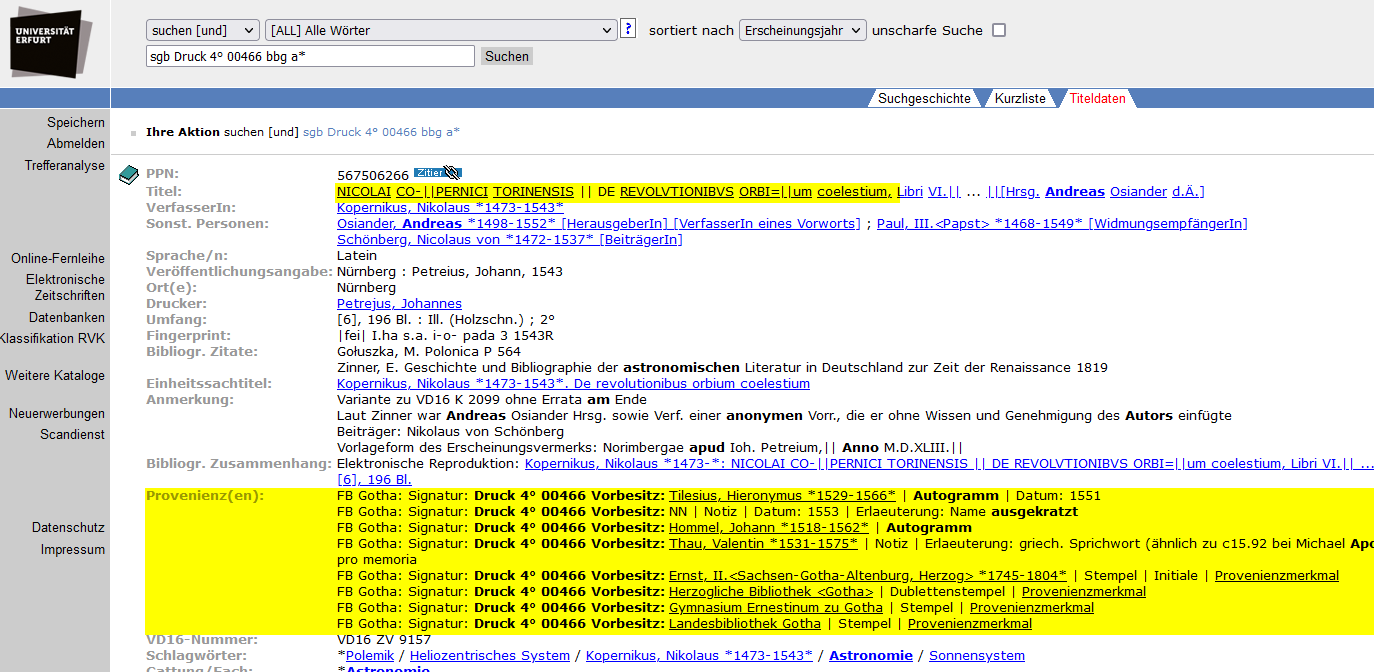
\includegraphics[width=\linewidth]{img/opac_derev_prov.png}
  \caption{University of Erfurt OPAC search result for exemplar \sig{Druck~4°~00466} of \enquote{De Revolutionibus} with provenance entries, screenshot of 2023-06-05}
  \label{fig:OPAC_derev_provenance}
\end{figure}

Our researcher can immediately decide that they can ignore the second entry (no name given) and the last three entries (corporate bodies).
For the persons named in the remaining four entries, our researcher finds the corresponding \gls{GND} records, which involves manual disambiguation in the case of Tilesius
\autocite{GNDTilesius,GNDHommel,GNDThau,GNDErnstII}.
%\footnote{%
%  \url{https://katalog.dnb.de/EN/home.html?v=plist}%
%}
On inspection of these \gls{GND} entries, it turns out that Ernest II was a regent and very probably not a scientist,
and that the other three people---Tilesius, Hommel, and Thau---had professions such as theologian,
mathematician, and astronomer, which qualifies them as scientists. Furthermore, Hommel's entry \todo{include screenshot}
contains a reference to Thau via the relation \term{student}, see Figure~\ref{fig:GND_Hommel}
(and Thau's entry contains the inverse reference to Hommel).
From this reference, our researcher can conclude that two scientists in the teacher-student relation
have both possessed the exemplar. 

\begin{figure}[ht]
  \centering
  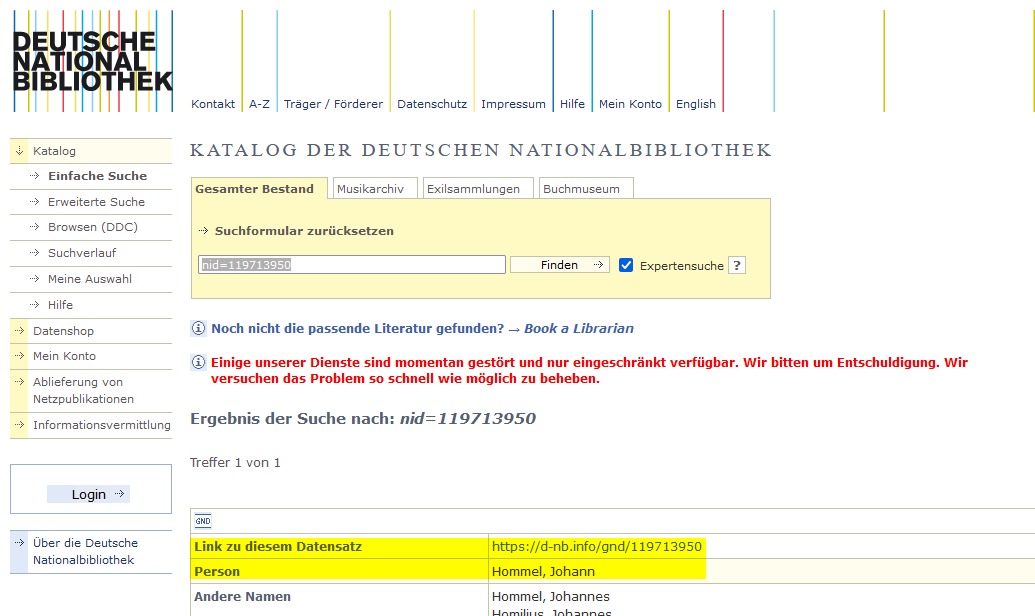
\includegraphics[width=\linewidth]{img/gnd_hommel_1.png}
  $\big[\raisebox{-1.8pt}{\rvdots}\big]$
  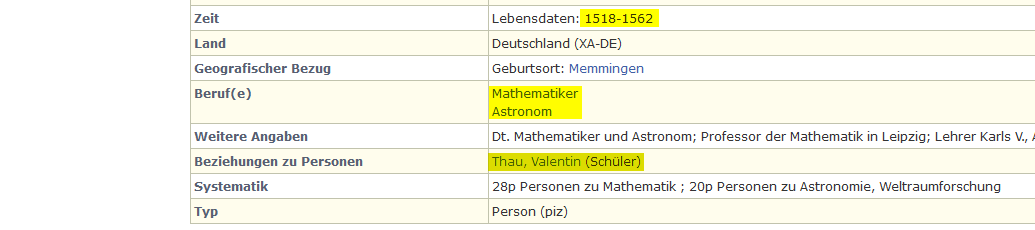
\includegraphics[width=\linewidth]{img/gnd_hommel_2.png}
  \caption{GND entry for Johann Hommel, screenshot of 2023-06-05}
  \label{fig:GND_Hommel}
\end{figure}

Unfortunately, the data available does not imply that Hommel passed the exemplar (directly) to Thau;
furthermore, the provenance entry for Thau raises doubts as to whether Thau was really an owner of the exemplar.
Therefore, the retrieved data can only be regarded as a \emph{candidate answer}
which entails the hypothesis that the found exemplar was passed from Hommel to Thau.
Our researcher can now engage in further research in order to verify that hypothesis.

\todo[think,inline]{Discuss specifics of \exaquery{1}, \exaquery{3}--\exaquery{9} (extend remarks from Section~\ref{sec:background})?}

% -----------------------------------------------------------------
\section{The Quality of Query Answers}
\label{sec:quality_of_answers}

Our simple example already illustrates that the quality of query answers
strongly depends on the quality of the underlying data,
regardless of whether answers are obtained manually or automatically. 
In particular, missing or spurious data will lead to missing or spurious answers.
Before we begin to deal with automated query answering,
we need to analyse the sources of missing or spurious data and their effects on the answers obtained.

For the sake of a principled discussion, we call the set of answers to a query obtained by some manual or automatic procedure
an \emph{answer set}, and we call the (set of) answers that the query has in reality the \emph{true answers} and the \emph{true answer set}.
In the above example, the answer set obtained by the described manual process consists of the single answer
\enquote{\sig{Druck~4°~00466}}, if we assume that our researcher interprets the data retrieved generously
(i.e., as an indication that Thau might have been an owner and might have received the book directly from Hommel)
and draws additional conclusions (i.e., that every mathematician or astronomer is a scientist).
The true answer set is not known and will most probably never be known; it is a term of rather philosophical nature.

Ideally, both answer sets should coincide.
Incomplete data may cause the answer set to exclude some true answers,
and spurious data may cause it to contain some answers that are not true.
We call the respective answers \emph{missing} and \emph{spurious}.
On the basis of our example, we can identify four distinct causes for data being incomplete or spurious,
as discussed in the following. We use the word \emph{term} as an umbrella term for concepts (such as \term{Scientist})
and relations (such as \term{student}).
%
\begin{enumerate}
  \item
    In the example, there is no information available in the \gls{GND} on whether any of the persons involved is indeed
    a \emph{scientist}. Instead, \gls{GND} provides information on more specific professions,
    e.g., for Thau and Hommel (theologian, mathematician, and astronomer).
    The information that they were scientists has to be \emph{derived} based on \emph{general knowledge
    of the world}.
    Indeed, a search in the \gls{GND} catalogue
    reveals that \gls{GND} does have an entry for the subject term \term{Wissenschaftler} (scientist) \autocite{GNDScientist}
    which, however, is used only sporadically: its 46 subordinate terms do not include, for example,
    \term{Mathematiker}, \term{Astronom}, or \term{Theologe} (mathematician, astronomer, theologian)  \autocite{GNDScientistSub}.
    
    The same effect can occur with relations instead of concepts:
    if \exaquery{2} were to ask for family members instead of collaborators or students
    but the data only supported more specific relations
    such as \term{sister} or \term{father}, then relationships using
    \term{familyMember} would need to be derived.
    Unfortunately, the cataloguing rules for \gls{GND} authority datasets do not require
    that relationships are recorded exhaustively nor using a normed vocabulary;
    see Section~\ref{sec:data_sources} for more details.
    
    In summary, terms can be missing in the data sources because
    they have not been recorded or because they are implicit in more specific terms.
    If the query uses such missing terms, then the answer set is always empty
    unless the person or machine determining the answers makes derivations based on their
    knowledge of the world.

%    Clearly, it would not be advisable to attempt adding all implicit knowledge to the data
%    because that would massively inflate the data,
%    as most terms have several superordinate concepts or relations and,
%    furthermore, implicit knowledge is not restricted to taxonomic knowledge.
%    \todo[think,inline]{Explain this further? A case for ontologies!}
  \item
    In the example, there is no information available on whether any of the owners of the exemplar
    \emph{passed it on} to another owner. Similarly,
    attempts to answer instances of Query Pattern~\exaquery{1} will have to deal
    with the problem that there is no information available as to who \emph{read} books.
    
    More generally speaking, terms can be missing in the data sources
    because they are not recorded at all, as a consequence of either a general lack of evidence
    or a general design decision for the data source. The underlying reasons can be manifold:
    for example, relationships such as who actually \emph{read} a book are very hard to confirm,
    or terms may not be part of the fixed vocabulary for a data field in a source.
    If the query uses such terms, then the answer set is always empty, as in Case~1.
  \item    
    In the example, it is possible that single owners of the exemplar or single relationships between owners
    have not been recorded because no evidence has been found yet.
    More generally, concept memberships or relationships can be missing sporadically,
    which may lead to missing answers.
  \item
    In the example, if Hommel is erroneously recorded as the owner, then the answer obtained on the grounds
    of that record is spurious.
    More generally, spurious concept memberships or relationships may lead to spurious answers.
\end{enumerate}
%
These cases reveal a striking qualitative difference concerning the effects of data incompleteness or spuriousness
on the answer set: Cases~3 and~4 have effects on single answers only, i.e., some answers are missing or spurious.
However, Cases~1 and~2 generally make \emph{all} answers missing unless further provisions are made.
Such \enquote{provisions} might include \emph{reasoning}
(e.g., deriving the implicit knowledge that Hommel was a scientist from the explicitly recorded fact that he was a mathematician)
and \emph{hypothesising} (e.g., assuming that Thau was an owner and received the book directly from Hommel).
Reasoning can be supported using semantic technologies such as (domain-specific or top-level) ontologies and related infrastructure.
A possible way to support hypothesising is to provide for the use of \emph{substitute information},
which has been addressed in the context of the \gls{SoNAR} project; see Section~\ref{sec:HNA+SoNAR}.
That is, users could be allowed to declare terms occurring in the data that may act as substitutes for certain terms used in their queries.

% Getting back to the general objective of this thesis, 
In the light of these observations,
it is appropriate to consider
query answers as \emph{candidates} that necessitate (and inspire) further research.
%as ....
For this purpose, spurious answers (in manageable numbers) are less harmful than missing answers.
Consequently, it is important to find ways to avoid missing answers without generating too many spurious answers.
In other words, it is desirable to obtain an answer set that is a slight \emph{overapproximation}
of the true answer set.

% -----------------------------------------------------------------
\section{From Manual to Automated Query Answering}
\label{sec:manual_vs_automated}

The manual process that we have described in Section~\ref{sec:manual_answering}
is cumbersome, laborious, and prone to errors and omissions for several reasons:
The search in library catalogues for exemplars of works and their provenances requires expert skills.
Catalogues with potential matches need to be selected manually,
and each catalogue needs to be queried individually, using its own search keys and syntax. 
%\todo[think]{give examples of commonalities (OPAC) and differences (discovery vs. OPAC)?}
For each retrieved exemplar, each potentially relevant provenance entry 
needs to be followed up in further data sources such as authority files,
multiplying the amount of manual work necessary.
Finally, it is not clear what an effective and efficient way to manually \enquote{explore}
relationships would be:
while it is easy to find direct relationships such as \term{student} in the view for a person's entry
in databases such as \gls{GND} or Wikidata, there are \emph{indirect} relationships
that are much harder to discover easily by hand,
e.g., \enquote{persons $P_1$ and $P_2$ are students of the same scholar}.

These considerations suggest that query answering will
strongly benefit from automated support,
which can help reduce the amount of manual work, integrate heterogeneous data sources,
incorporate background knowledge (e.g., every mathematician is a scientist),
and discover indirect relationships between entities or \enquote{substitute information}.
We envisage a retrieval system that enables researchers to formulate queries 
and which computes answers consulting data sources selected by the user.
The vocabulary used for formulating queries should be based on the vocabulary
present in the data sources, but it should also include concepts and relations
such as \term{scientist} or \term{read},
which are not recorded in the data, as discussed in
Section~\ref{sec:quality_of_answers}. The retrieval system thus needs to implement ways
to match those terms with the available vocabulary, as well as techniques
for integrating data from heterogeneous sources.
It is our general vision that the retrieval system will serve as an instrument for prospectively finding interesting
candidates that inspire further research.
In the remainder of this thesis, we want to lay the foundations and develop a precise method
that can serve as a basis for a future implementation of a retrieval system.


  % !TeX spellcheck = en_GB
% =================================================================
\chapter{Analysis of Available Data Sources and Techniques}
\label{chap:analysis}

In order to build a system for retrieving provenance relationships,
data sources need to be selected. It is the aim of this chapter
to provide information for this selection can be based later on.
Furthermore, the abstract model of data sources, provenance queries, and answers
that we will develop in the following chapter
needs to incorporate the characteristics of the data models used in the appropriate data sources.
For this purpose, we review data sources that contain the relevant metadata (Section~\ref{sec:data_sources}),
as well as bibliographic standards, data formats, and communication interfaces
relevant for these sources (Sections~\ref{sec:bib_standards} and~\ref{sec:data_models}).
Given the observation from the previous chapters
that answering provenance queries is likely to involve several data sources,
we pay special attention to data transfer and integration techniques,
including linked data.
At the end of this chapter (Section~\ref{sec:implications_on_modelling}),
we draw conclusions from the review that inform our model and method in the following chapters.

Before we start the review, we need to define the central term \emph{metadata}.
For this purpose, we follow \citeauthor{Hider2008}'s \autocite*{Hider2008} definition and reflection:
The term \emph{metadata} is used in multiple ways.
The most general use is according to its literal meaning, \enquote{data about data}.
This definition is not restricted to the library domain
but includes bibliographic records for documents (which contain the primary \emph{data}).
A more specific variant is the use of \enquote{metadata} to refer to
structured data describing digital objects,
again independently of the library domain. \citeauthor{Hider2008} also note that
these two meanings can no longer be clearly distinguished in view of the
progressing digital transformation. In this thesis, we adopt their
decision to use the term \emph{metadata} in the most general sense,
\enquote{applying to all information resources} \autocite[p.13]{Hider2008}.

% -----------------------------------------------------------------
\section{Standards for the Description of Bibliographic Resources}
\label{sec:bib_standards}


The following two standards are widely adhered to in bibliographic data sources.
This discussion
is a brief summary of \citeauthor{Wiesenmueller2015}'s introduction
\autocite*[§§2,3]{Wiesenmueller2015},
unless indicated otherwise.

% .............
\paragraph{FRBR}

The \gls{FRBR} constitute a conceptual entity-relationship model
developed by the \gls{IFLA} in 1998 (and updated in 2009)
in order to support users in finding, identifying, selecting, and accessing
bibliographic items \autocite[p.17]{Wiesenmueller2015}.
\gls{FRBR}'s entities represent things that need to be represented in the data.
These entities fall into three groups, of which we introduce the first
two.
Entities of Group~1 are \term{Work}, \term{Expression}, \term{Manifestation}, \term{Item},
and their common superordinate concept \term{Endeavour};
entities of Group~2 are \term{Person}, \term{CorporateBody},
and their superordinate concept \term{ResponsibleEntity}.
Furthermore, \gls{FRBR} contains relations that link Group-1 entities with each other
and with Group-2 entities, respectively.
These entities and the basic relations are shown in Figure~\ref{fig:FRBR}.

%\begin{figure}[ht]
%  \centering
%  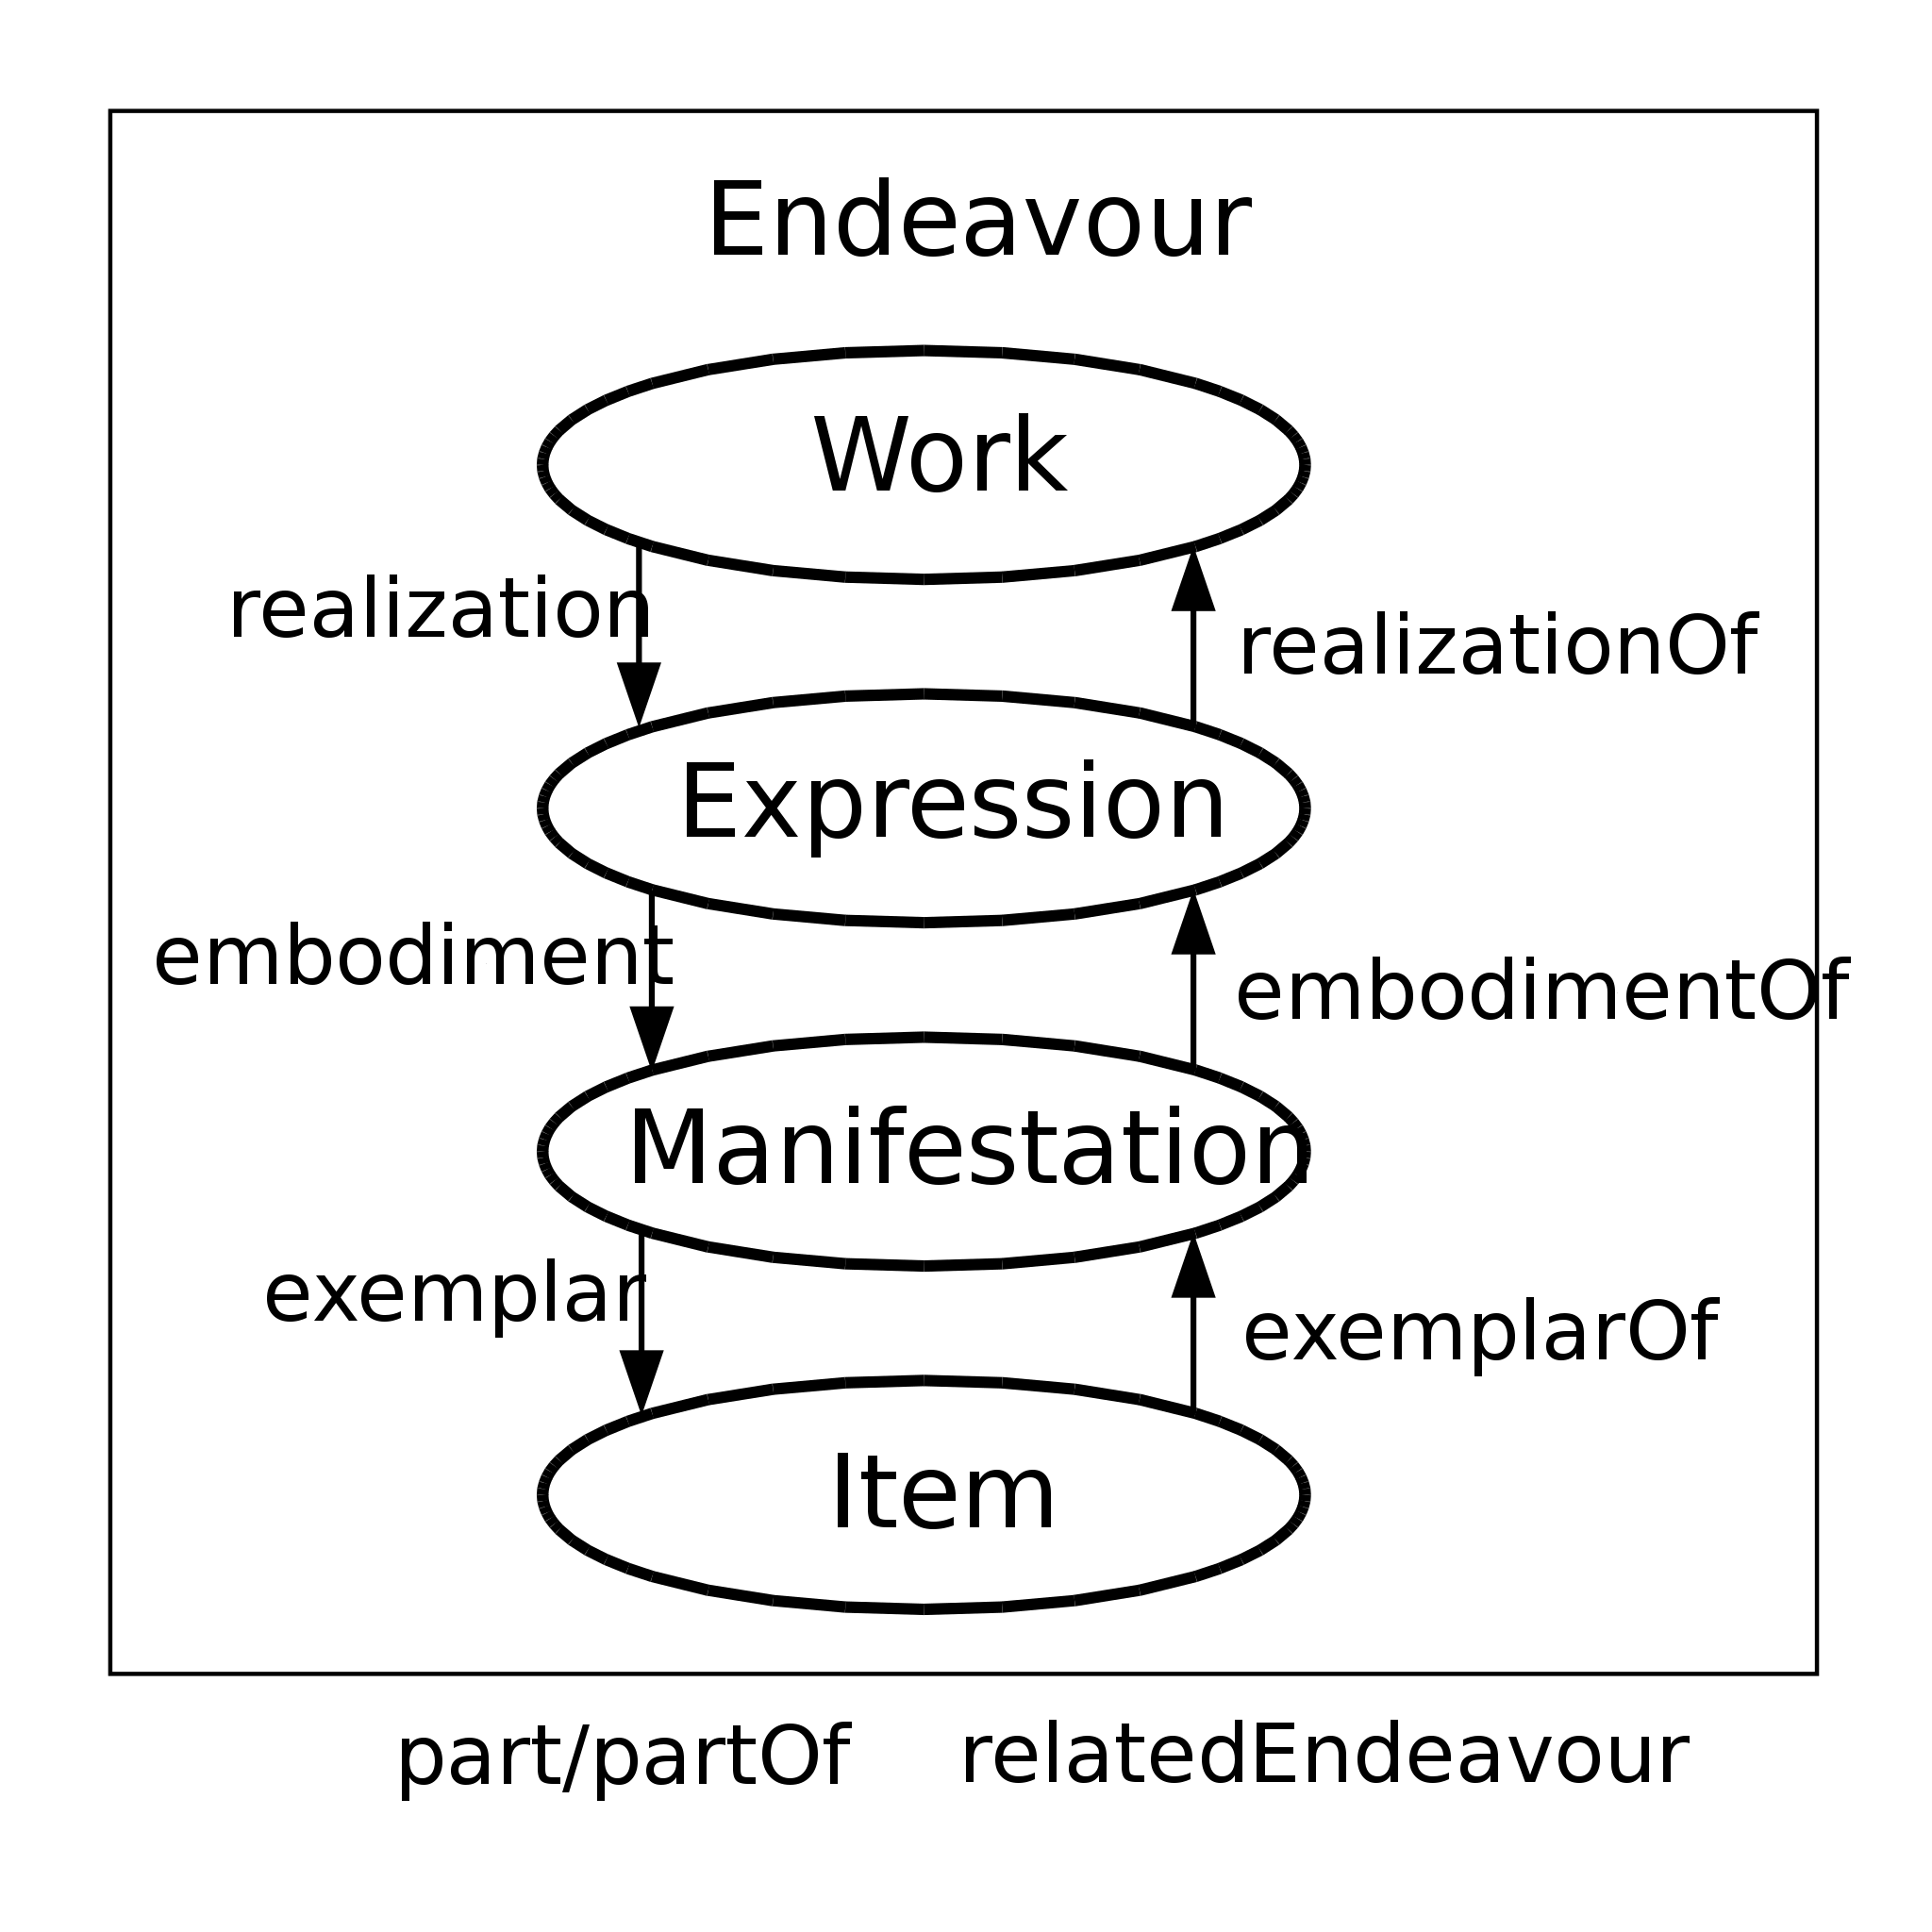
\includegraphics[height=60mm]{img/FRBR_Group1.png}
%  \qquad
%  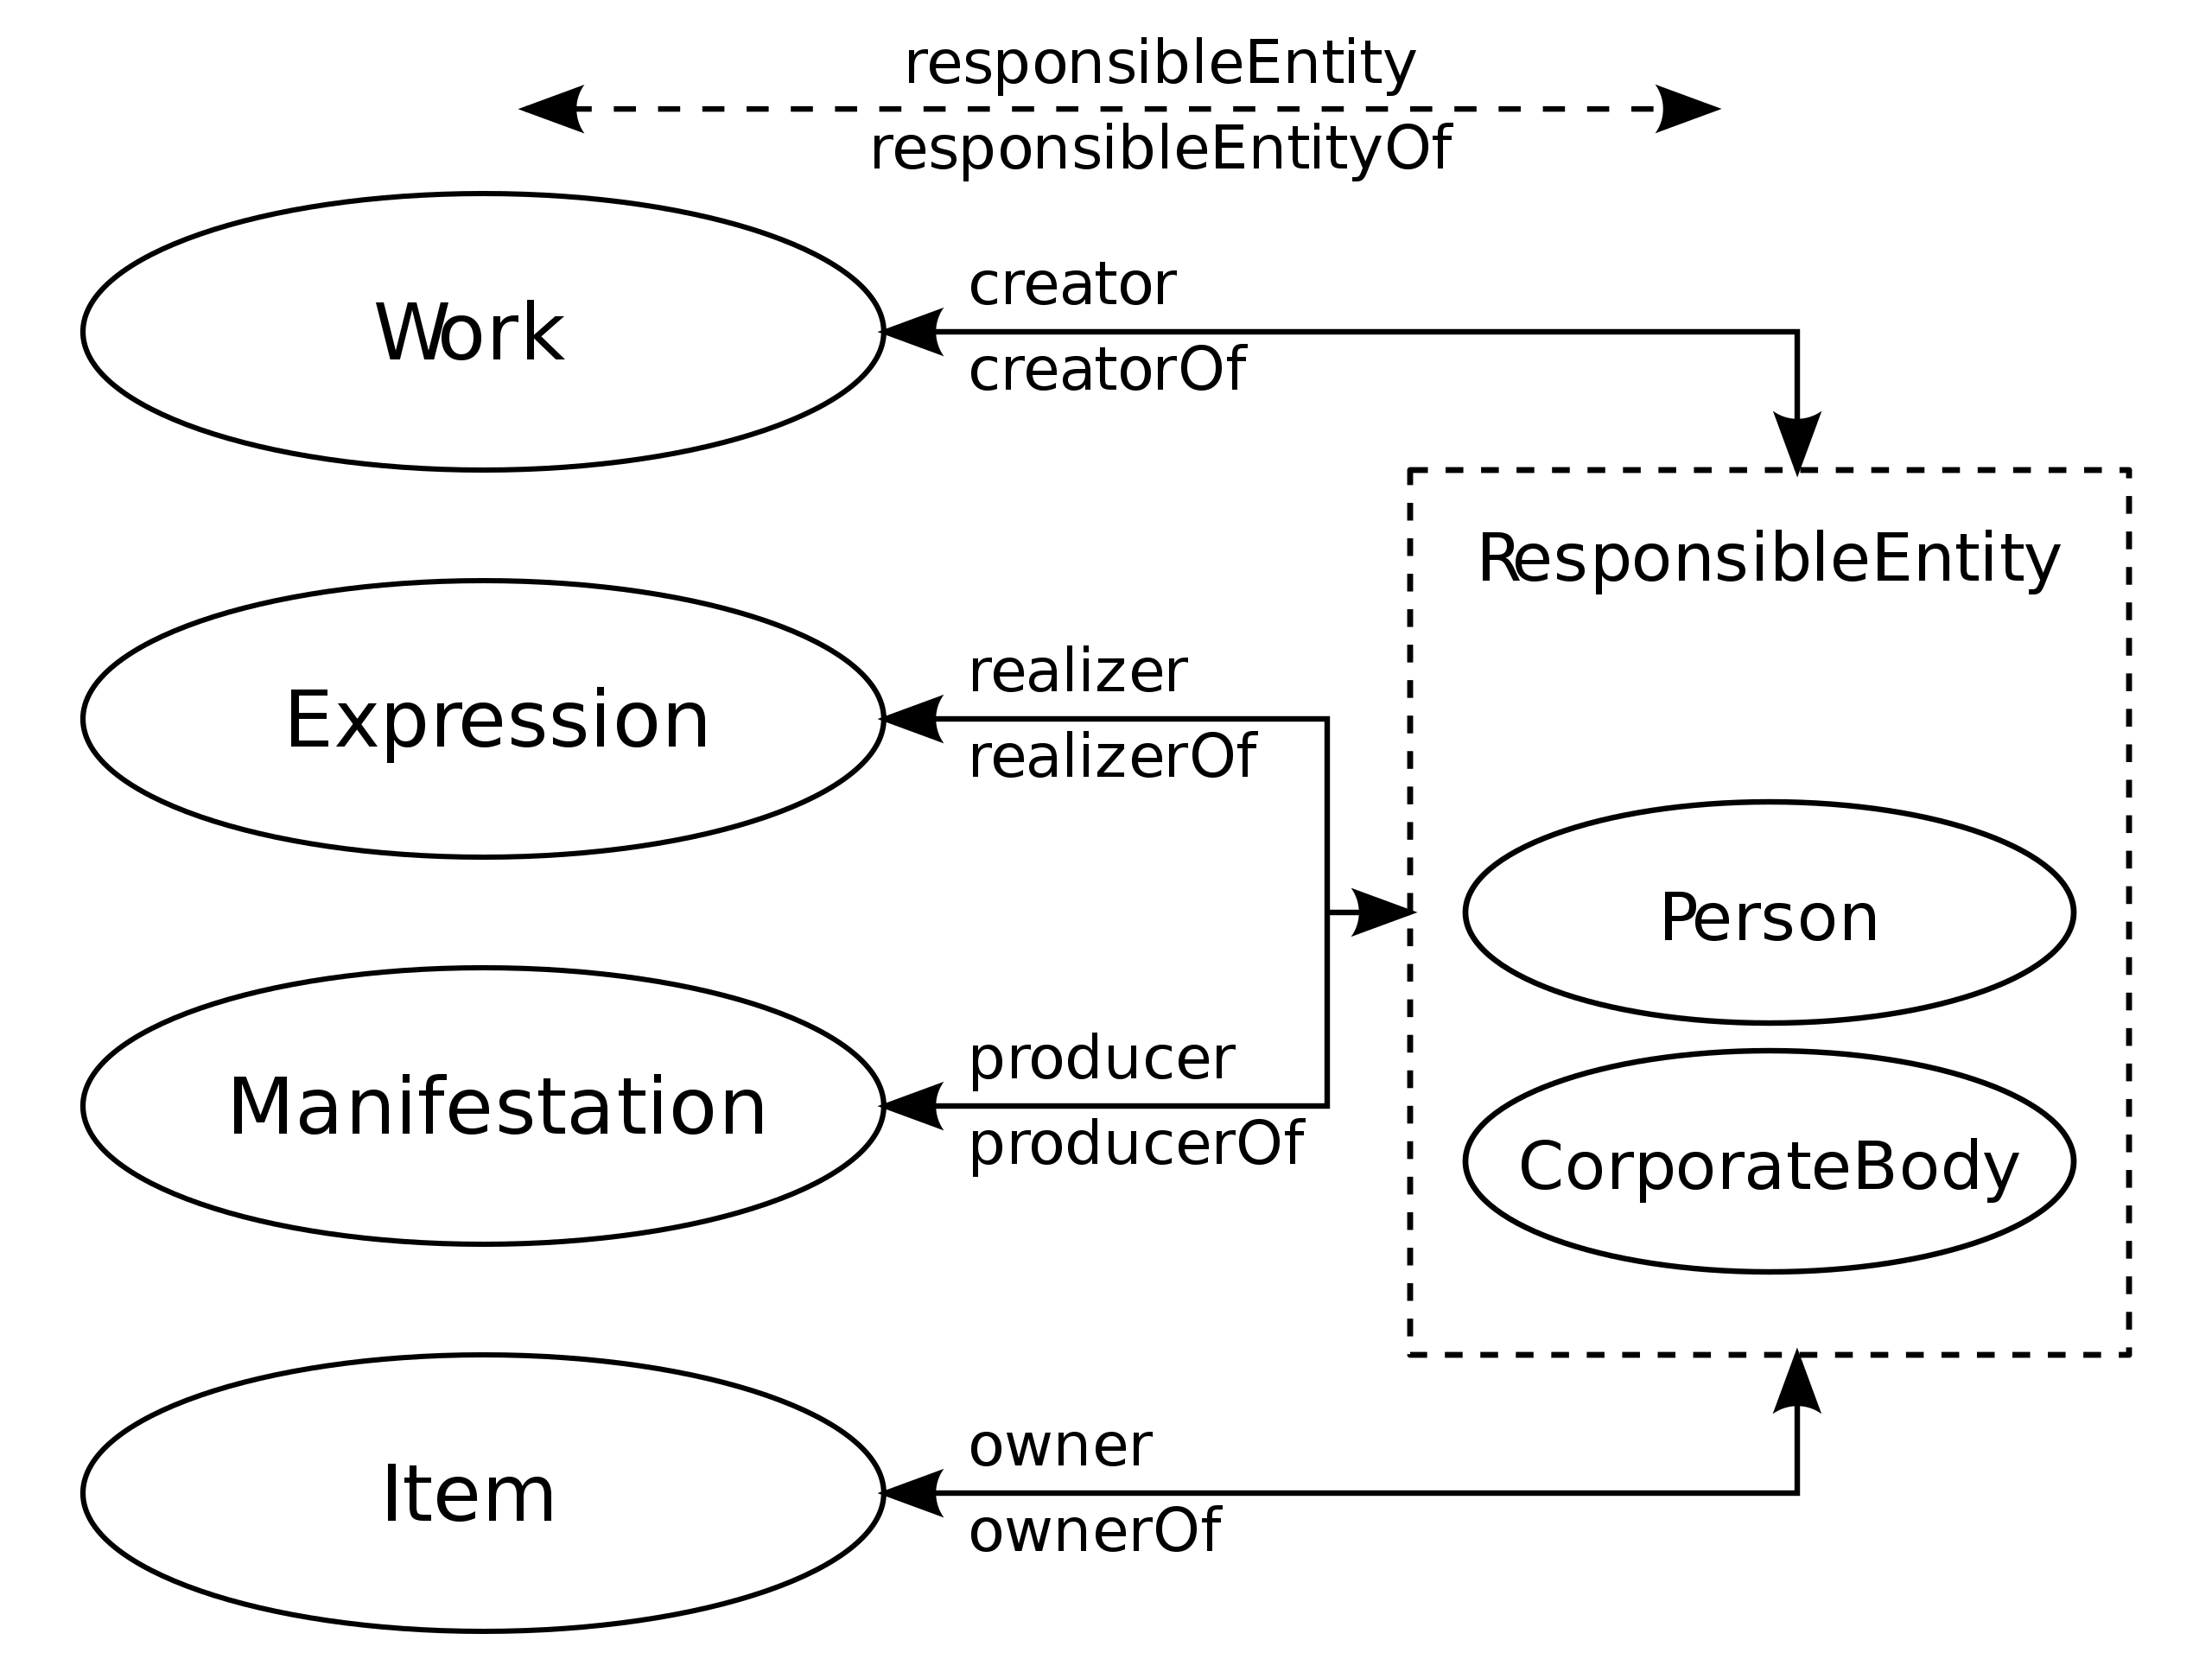
\includegraphics[height=60mm]{img/FRBR_Group2.png}
%  
%  \todo[defer,inline]{Make better picture? (see draft)}
%  
%  \caption[Basic FRBR entities and relations of Group~1 and Group~2]{%
%    \parbox[t]{.85\linewidth}{%
%      Basic \gls{FRBR} entities and relations of Group~1 (left) and Group~2 (right)
%      \par
%      \begin{footnotesize}
%        \href{https://commons.wikimedia.org/wiki/File:FRBR-Group-1-entities-and-basic-relations.svg}{\enquote{Basic Group 1 entities and relations of the FRBR model (RDF version)}} and
%        \href{https://commons.wikimedia.org/wiki/File:FRBR-Group-2-entities-and-relations.svg}{\enquote{Basic Group 2 entities and relations of the FRBR model (RDF version)}}
%        by \href{https://commons.wikimedia.org/wiki/User:JakobVoss}{Jakob Voss} are licenced under \href{https://creativecommons.org/licenses/by-sa/4.0/}{CC BY-SA 4.0}.
%        \par
%      \end{footnotesize}
%    }%
%  }
%%  \label{fig:FRBR}
%\end{figure}
%
\newlength{\manif}\settowidth{\manif}{\fns Manifestation}%
\newlength{\respe}\settowidth{\respe}{\fns ResponsibleEntity}%
\begin{figure}[ht]
  \centering
  \begin{tikzpicture}[
    >=Latex,
    every node/.style={on grid,rectangle,rounded corners=1mm,draw=black,fill=lightblue,thick,inner sep=1.5mm},
    every edge/.style={draw=black,thick}
  ]
    % the 4 Group-1 entities
    \node                       (Work) {\fns\mystrut\tikzpb[\hspace*{\fill}]{\manif}{\term{Work}}};
    \node [below=12mm of Work]  (Expr) {\fns\mystrut\tikzpb[\hspace*{\fill}]{\manif}{\term{Expression}}};
    \node [below=12mm of Expr]  (Mani) {\fns\mystrut\tikzpb[\hspace*{\fill}]{\manif}{\term{Manifestation}}};
    \node [below=12mm of Mani]  (Item) {\fns\mystrut\tikzpb[\hspace*{\fill}]{\manif}{\term{Item}}};
    
    % their superterm Endeavour
    \node [above=11mm of Work, draw=none,fill=none,inner sep=0mm] (Ende) {\fns\mystrut\tikzpb[\hspace*{\fill}]{\manif}{\term{Endeavour}}};

    % placeholders plus rectangle for Endeavour
    \node [above left =1mm and 1mm of Work.north west,draw=none,fill=none,inner sep=.2mm] (WorkL) {};
    \node [below right=0mm and 1mm of Item.south east,draw=none,fill=none,inner sep=.2mm] (ItemR) {};
    \node [fit={(Ende) (WorkL) (ItemR)},fill=none] (G1E) {};
    
    % super-relations of Group-1 relations
    \node [left =8mm of Ende.180,draw=none,fill=none,inner sep=0mm] () {\fns\tikztabtwo[r]{\term{relatedEndeavour,}}{\term{part}}};
    \node [right=8mm of Ende.0  ,draw=none,fill=none,inner sep=0mm] () {\fns\tikztabtwo[l]{\term{relatedEndeavour,}}{\term{partOf}}};
    
    % the 2 Group-2 relations
%    \node [right=98mm of Expr] (Pers) {\fns\mystrut\tikzpb[\hspace*{\fill}]{\respe}{\term{Person}}};
%    \node [below= 8mm of Pers] (Corp) {\fns\mystrut\tikzpb[\hspace*{\fill}]{\respe}{\term{CorporateBody}}};
    \node [right=98mm of Item] (Corp) {\fns\mystrut\tikzpb[\hspace*{\fill}]{\respe}{\term{CorporateBody}}};
    \node [above= 8mm of Corp] (Pers) {\fns\mystrut\tikzpb[\hspace*{\fill}]{\respe}{\term{Person}}};

    % their superterm ResponsibleEntity
    \node [right=98mm of Ende, draw=none,fill=none,inner sep=0mm] (Resp) {\fns\mystrut\tikzpb[\hspace*{\fill}]{\respe}{\term{ResponsibleEntity}}};

    % placeholders plus rectangle for ResponsibleEntity
    \node [above left =1mm and 0mm of Pers.north west,draw=none,fill=none,inner sep=.2mm] (PersL) {};
    \node [below right=0mm and 0mm of Corp.south east,draw=none,fill=none,inner sep=.2mm] (CorpR) {};
    \node [fit={(Resp) (PersL) (CorpR)},fill=none] (G2E) {};

    % super-relations of Group-2 relations
    \node [left=6mm of Resp.180,draw=none,fill=none,inner sep=0mm] () {\fns\tikztabtwo[r]{\term{responsibleEntity/}}{\term{responsibleEntityOf}}};
    
    % placeholders for separating line
    \node [above=2mm of $(G1E.north east)!0.50!(G2E.north west)$,draw=none,fill=none,inner sep=.2mm] (SepN) {};
    \node [below=5mm of $(G1E.south east)!0.50!(G2E.south west)$,draw=none,fill=none,inner sep=.2mm] (SepS) {};
    
    \begin{scope}[%
      every node/.style={draw=none,fill=none,inner sep=.2mm}
    ]
      % Labels for groups
      \node [above  left=0mm and 2mm of SepS] () {\small Group 1};
      \node [above right=0mm and 2mm of SepS] () {\small Group 2};
      
      \path[->]
        % the 3 main Group-1 relations
        (Work) edge[out=195,in=165,looseness=3] node[left=1mm] {\fns\mystrut\term{realization}} (Expr)
        (Expr) edge[out=195,in=165,looseness=3] node[left=1mm] {\fns\mystrut\term{embodiment}}  (Mani)
        (Mani) edge[out=195,in=165,looseness=3] node[left=1mm] {\fns\mystrut\term{exemplar}}    (Item)
        
        % and their inverses
        (Expr) edge[out=15,in=345,looseness=3] node[right=1mm] {\fns\mystrut\term{realizationOf}} (Work)
        (Mani) edge[out=15,in=345,looseness=3] node[right=1mm] {\fns\mystrut\term{embodimentOf}}  (Expr)
        (Item) edge[out=15,in=345,looseness=3] node[right=1mm] {\fns\mystrut\term{exemplarOf}}    (Mani)
        
        % Group-2 relations
%        (Work) edge[out=5,in=150]  node[pos=.98,above left=1mm and 1mm,sloped] {\fns\mystrut\term{creator}}   (G2E)
%        (G2E)  edge[out=160,in=-5] node[pos=.02,below left=1mm and 1mm,sloped] {\fns\mystrut\term{creatorOf}} (Work)
        (Work.4)   edge node[pos=.98,above left=.2mm and 1mm] {\fns\mystrut\term{creator}}  ($(G2E.north west)!(Work.4)!(G2E.south west)$)
        (Expr.4)   edge node[pos=.98,above left=.2mm and 1mm] {\fns\mystrut\term{realizer}} ($(G2E.north west)!(Expr.4)!(G2E.south west)$)
        (Mani.4)   edge node[pos=.98,above left=.2mm and 1mm] {\fns\mystrut\term{producer}} ($(G2E.north west)!(Mani.4)!(G2E.south west)$)
        (Item.4)   edge node[pos=.98,above left=.2mm and 1mm] {\fns\mystrut\term{owner}}    ($(G2E.north west)!(Item.4)!(G2E.south west)$)

        % and their inverses
        ($(G2E.north west)!(Work.356)!(G2E.south west)$) edge node[pos=.02,below left=.2mm and 1mm] {\fns\mystrut\term{creatorOf}}  (Work.356)
        ($(G2E.north west)!(Expr.356)!(G2E.south west)$) edge node[pos=.02,below left=.2mm and 1mm] {\fns\mystrut\term{realizerOf}} (Expr.356)
        ($(G2E.north west)!(Mani.356)!(G2E.south west)$) edge node[pos=.02,below left=.2mm and 1mm] {\fns\mystrut\term{producerOf}} (Mani.356)
        ($(G2E.north west)!(Item.356)!(G2E.south west)$) edge node[pos=.02,below left=.2mm and 1mm] {\fns\mystrut\term{ownerOf}}    (Item.356)
      ;
    \end{scope}
    
    % draw separating line
    \path[-,dash pattern={on 6pt off 3pt}] (SepN) edge (SepS);
%        
  \end{tikzpicture}
  
%  \caption[Basic FRBR entities and relations of Group~1 and Group~2]{%
%    \parbox[t]{.85\linewidth}{%
%      Basic \gls{FRBR} entities and relations of Group~1 (left) and Group~2 (right)%
%    }%
%  }
  \caption[FRBR entities and basic relations of Groups~1 and~2]{\gls{FRBR} entities and basic relations of Groups~1 and~2 \autocite[following][]{FRBRpic1,FRBRpic2}}
  \label{fig:FRBR}
\end{figure}

Beside FRBR, the \gls{IFLA} developed
a conceptual entity-relationship model for authority data,
the \gls{FRAD},
as well as a continuation of FRBR,
the \gls{FRSAD}.

FRBR serves as a basic principle of RDA, which we discuss next.

% .............
\paragraph{RDA}

\gls{RDA} is a standard for the cataloguing of publications
in cultural heritage institutions, and particularly in libraries.
RDA is implemented and used in the library systems of several countries, including
the US, the UK, Canada, Australia, and the German-speaking countries
\autocite{WikiDE_RDA}.

RDA and the application guidelines for the German-speaking area
stipulate a special practice for recording FRBR Group-1 entities and relating 
them to each other: Bibliographic records (\enquote{Titel\-daten\-sätze})
have a bibliographic level for describing a manifestation
and an exemplar level for describing the related exemplars. The description of works and expressions
is considered part of the description of a manifestation and thus recorded on the bibliographic level.
However, it is possible to create and link an authority record for a work or expression
containing the relevant description. In that case, the source of the information can be recorded as well
\autocite[cf.][§5.1]{Wiesenmueller2015}.

For our approach, this observation means that catalogues of German libraries
do not use a uniform way of linking, e.g., a work $X$ with its manifestations.
In particular, if there is no authority record for $X$,
then $X$ is represented in the data of its manifestations only implicitly 
(and possibly ambiguously).


% -----------------------------------------------------------------
\section{Data Formats and Communication Protocols}
\label{sec:data_models}

In order to identify data sources in the following section,
we first need to describe relevant standards and formats for the description
and communication of (bibliographic) data.
The following discussion 
is based on~\citeauthor{Hider2008}'s overview \autocite*[§10]{Hider2008},
unless indicated otherwise

% - - - - - - - - - - - - - - - - - - - - - - - - - - - - - - - - -
\subsection{Markup Languages}
\label{subsec:markup}

We briefly describe markup languages, which are repeatedly used in the technologies
described in the following subsections.
Markup languages are machine-readable languages used for the structuring and formatting of files.

% .................
\paragraph{HTML}
The most prominent example is the \gls{HTML}, the core language of the \gls{WWW}.
The markup features of HTML are also used to identify and describe certain elements of digital objects.
In particular, HTML provides for meta tags, i.e., labels for metadata.
One of the restrictions of HTML is its fixed set of labels, whose meanings cannot be changed.
Further standards were developed to overcome this restriction,
such as SGML and XML.

% .................
\paragraph{XML}
\glsreset{XML}%
The \gls{XML} is both a file format and markup language for the storage and transmission of arbitrary data;
it allows for a hierarchical structuring of data in a text file format that is readable by both humans and machines
\autocite{WikiXML}.
XML is the basis for many modern web developments.
Most metadata schemas have standard expressions in XML, as we will learn below.

% - - - - - - - - - - - - - - - - - - - - - - - - - - - - - - - - -
\subsection{Data Communication Protocols}
\label{subsec:data_comm_prot}

% .............
\paragraph{Z39.50}

\glsreset{Z39.50}
is a protocol for data communication between bibliographic databases.
\glsunset{ISO}%
\glsunset{ANSI}%
\glsunset{NISO}%
It is an \gls{ISO} standard as well as an \gls{ANSI}/\gls{NISO} standard.
\glsunset{Z39.50}%
Z39.50 is a set of rules developed specifically
for translating search and retrieval commands between databases such as OPACs.
Using Z39.50, it is possible to issue commands specific to a local database
and obtain results from a remote database that uses a possibly different command set.
This protocol can be implemented over the internet and similar networks.
Z39.50 is widely used in the library domain for providing access to catalogues,
for example, by the \gls{LoC}. Still, it is not fully implemented by all library systems,
and not all libraries use the most recent version. It is also not very widely spread
outside the library community.

% .............
\paragraph{SRU}

\gls{SRU} is a successor of \gls{Z39.50} and an \gls{LoC} standard.
It has the same function, which is the standardisation of search and retrieval
across online databases. 
SRU is based on \gls{HTTP}, \gls{XML}, and the \gls{CQL}, 
a standard syntax for representing queries to information retrieval systems.
Thanks to this technology, SRU is more dynamic than \gls{Z39.50}
and less restricted to the library domain.

% .............
\paragraph{OAI-PMH}

The \gls{OAI} is a project devoted to interoperability standards in information agencies
in general, including libraries.
The \gls{OAI-PMH} is a standard developed by the OAI
and is widely used in the library domain, albeit not as widely as \gls{Z39.50}.

% - - - - - - - - - - - - - - - - - - - - - - - - - - - - - - - - -
\subsection{Data Description Schemata}
\label{subsec:data_descr_schemata}

% .............
\paragraph{MARC}

\glsreset{MARC}
\gls{MARC} \enquote{is the main data communication standard in use in libraries today}
\autocite[p.198]{Hider2008}. It is a family of formats for the exchange of bibliographic
and further data between library systems, which is being extensively used by libraries around the world. 
MARC was developed by the \gls{LoC} in 1969
and has been updated several times.
The MARC family comprises more than 20 dialects that have been developed as an official standard
in several countries.
Those are very similar to each other and provide very detailed record structures for cataloguing of bibliographic data.
They all adhere to an international \gls{ISO} standard.
The development of MARC pursued the goals of labour and cost reduction,
and of standardising the cataloguing process
as well as data communication and transfer.
MARC \enquote{allows flexibility in library information systems} \autocite[p.201]{Hider2008}
by providing an easy way of data exchange and allowing for better resource discovery (among others, in comprehensive union catalogues).

MARC~21, was developed in 1999 and is \enquote{the major version of MARC in use internationally} \autocite[p.205]{Hider2008}.
It consists of five formats for specific kinds of data.
Two of these are for bibliographic data and authorities data, respectively.

MARC has been criticised for its inflexible structure, the fragmentation into several dialects,
and the restricted compatibility with current computer technologies, among other things.
\textcite[p.212]{Hider2008} give more details and further references.
There have been several attempts to redeem some of these disadvantages,
among them the development of new standards such as MODS (see below)
and of \gls{XML} schemas based on MARC~21 such as MARCXML and Turbomarc.

The problem of standard proliferation was not restricted to the
variety of MARC dialects but also occurred within non-MARC formats.
Attempts to solve this problem have been made via
translation and unification. One tool for unification is Dublin Core (DC); see below.

% .............
\paragraph{MAB}

The \gls{MAB}, translating as \enquote{machine data exchange format for libraries},
is a legacy bibliographic data format that has been developed solely for the purpose of data exchange
by the \gls{DNB}.
Although \textcite[p.204]{Hider2008} classify it as a dialect of \gls{MARC},
it is in fact conceptually different from \gls{MARC},
assigning exactly one bibliographic element to each data field
and allowing a more flexible ordering of elements \autocite{WikiMAB}.
In 2013, the \gls{DNB} completely abandoned the delivery of its bibliographic and authority data in MAB
in favour of \gls{MARC}~21 \autocite{MAB}.

% .............
\paragraph{MODS}

The \gls{MODS} is a standard developed by the \gls{LoC}
in order to overcome the problems with \gls{MARC} mentioned above.
MODS is based on \gls{XML} and a subset of MARC fields;
it can thus be used alongside MARC and as a \enquote{switching format
between MARC and non-MARC schemas} \autocite[p.219]{Hider2008}.
The LoC also maintains an analogous standard for authority data,
the \gls{MADS}.

% .............
\paragraph{DC}

\gls{DC} is an international standard consisting of 15 essential metadata terms
for describing digital or physical resources.
It was formulated by the \gls{DCMI}, a project of the US-American non-profit organisation
ASIS\&T, for the purpose of locating information resources on the \gls{WWW}.
The 15 core elements are tailored towards the \enquote{primary metadata needs} across domains
\autocite[p.215]{Hider2008}, thus making it a flexible data model.
Applications of \gls{DC} include resource description,
the combination of metadata vocabularies from different standards,
and the provision of interoperability in the linked data context.
\gls{DC} is extended by the \emph{DCMI Metadata Terms}.

%Sources of this summary are \textcite[§§1, 10]{Hider2008},
%and \citeauthor{WikiDC}~\autocite{WikiDC}.

% .............
\paragraph{RDF}

We have already introduced \gls{RDF} in Section~\ref{sec:linked_data+integration}.
In the context of the following description of data sources,
RDF is a very flexible data schema and the core technology for providing metadata as linked data.

% .............
\paragraph{BIBFRAME}

The \gls{BIBFRAME} is a data model for bibliographic description,
which was designed to replace the \gls{MARC} standards and use linked data principles
to improve access to bibliographic metadata within and outside the library domain \autocite{WikiBIBFRAME}.
The most recent version 2.0 was released by the \gls{LoC} in 2016 \autocite{BIBFRAME}.
So far, only a handful of libraries are using BIBFRAME,
most of them in test mode \autocite{WikiBIBFRAME}.

% -----------------------------------------------------------------
\section{Data Sources}
\label{sec:data_sources}

In this section, we provide information on data sources
that provide metadata on objects and individuals
relevant for provenance research, such as works, expressions, manifestations, exemplars,
persons, ownership, and social relationships.
We first give an overview of eligible data sources (Subsection~\ref{subsec:collection_data_sources})
and then select a few particularly relevant ones, for which we provide a detailed analysis
(Subsection~\ref{subsec:analysis_data_sources}).
The choice of the latter was motivated by the insights from the \gls{SoNAR} project (see Section~\ref{sec:HNA+SoNAR})
and Hakelberg's \autocite*[§4]{Hakelberg2016} overview of the state of provenance indexing with authority data
in the German-speaking area. This analysis will have to be extended
whenever the model and method that we are going to develop in the following chapters
is implemented in a retrieval system in future work.

% - - - - - - - - - - - - - - - - - - - - - - - -
\subsection{Collection of Data Sources}
\label{subsec:collection_data_sources}

We have identified four categories of relevant data sources:
library catalogues, special databases for provenance research, authority files, and knowledge bases.
We next describe, for each of these categories, the relevant information that is
contained in the respective data sources, and we list examples.

% .............
\paragraph{Library Catalogues}
%
%Library catalogues 
Catalogues contain the information relevant for provenance research, such as
%
\begin{itemize}
  \item
    bibliographic entities (works, manifestations, expressions, exemplars);
  \item
    relations between these entities (e.g., \term{isManifestationOf});
  \item
    attributes for these entities (e.g., year of publication);
  \item
    people and corporate bodies and relations such as authorship;
  \item
    provenance entries (including, e.g., owners, the ownership relation, and further attributes such as the year of ownership);
  \item
    (implicitly) the current ownership;
  \item
    (ideally) references to entries in authority files for all these types of entities.
\end{itemize}
%
Examples of relevant library catalogues include
%
\begin{itemize}
  \item
    catalogues of national libraries, which often aim at collecting literature exhaustively
    and which are most likely to make metadata available in interoperable formats,
    in particular: \\
    \mybold{the catalogues of \gls{DNB}, \gls{LoC}, and the British Library} \autocite{DNBCatalogue,LoCcatalogue,BLcatalogue};
  \item
    meta-catalogues that enable a federated search in several catalogues,
    in particular: \\
    \glsunset{KVK}%
    \mybold{WorldCat} and the \mybold{\glsentrylong{KVK} (\gls{KVK})} \autocite{WorldCat,KVK};
  \item
    catalogues of (German) library networks,
    in particular: \\
    \glsunset{B3KAT}
    \glsunset{hbz}%
    \glsunset{hebis}%
    \mybold{\gls{K10plus}, \gls{B3KAT},}
    the \mybold{union catalogues of \gls{hbz} and \gls{hebis}} \autocite{K10plus,B3KAT,hbz,hebis};
  \item
    catalogues of single libraries, if not covered by any of the above;
  \item
    special catalogues, e.g., those used for historical research in the \gls{SoNAR} project, %\todo{explain; relate to SoNAR or loot research}
    in particular: \\
    \mybold{\gls{ZDB}, \gls{KPE}, \gls{ZEFYS}, ExilePress} \autocite{ZDB,KPE,ZEFYS,ExilePress}.
\end{itemize}

% .............
\paragraph{Authority Files}
%
Authority files
contain information relevant for provenance research, such as
%
\begin{itemize}
  \item
    entities such as persons, corporate bodies, places, works;
  \item
    relations such as social relations, family relations, professional relations;
  \item
    attributes for the entities such as their profession;
\end{itemize}
%
They are usually subject to a strict quality control.
Examples include the \mybold{\gls{GND}} \autocite{GND} in the German-speaking area (which has been used extensively in \gls{SoNAR}),
the North-American \mybold{\gls{LCNAF}} \autocite{LCNAF},
and the international projects \mybold{\gls{ISNI} and \gls{VIAF}} \autocite{ISNI,VIAF}.

% .............
\paragraph{Knowledge Bases}

According to the insights from the \gls{SoNAR} project,
(open) \glspl{KB} can be useful when trying to overcome the problem with missing or unbalanced data
in authority files such as the \gls{GND} (see Section~\ref{sec:HNA+SoNAR}).
\Glspl{KB} are usually edited independently of the library domain by a wider community of contributors,
and their quality cannot be expected to meet the standards of catalogues or authority files edited by library personnel.
A prominent example of an open, cross-domain \gls{KB} is \mybold{Wikidata} \autocite{Wikidata},
which has tentatively been used in the context of the \gls{SoNAR} project
and which we have already identified in Section~\ref{sec:background} as possible source of metadata
for complementing authority data.

% .............
\paragraph{Cultural Heritage Databases}

This category contains generic federated portals of cultural heritage items
as well as special databases created especially for the support of provenance research.
Examples for these two kinds of databases are, respectively, \mybold{Europeana} \autocite{Europeana} (see Section~\ref{sec:linked_data+integration})
and \mybold{Proveana}---the research database of the German Lost Art Foundation \autocite{Proveana}.

% - - - - - - - - - - - - - - - - - - - - - - - -
\subsection{Analysis of Data Sources}
\label{subsec:analysis_data_sources}

We now provide a review of four data sources from the previous list, namely
\gls{DNB}, \gls{K10plus}, \gls{GND}, and Wikidata.
%\gls{KVK}, \gls{ZDB}, \gls{KPE}, Proveana, Europeana.
%
%The main goal of this analysis is to provide an exemplary overview of the features and specifics
%of these data sources, and to inform the model that we will develop in the subsequent chapter.
%In order to fulfil this purpose, it is not necessary to review all data sources listed above
%exhaustively.
%
%\todo[inline]{adapt this list and provide another brief justification for the choice?}
%
For each data source, we collect the following information.
%
\begin{itemize}
  \item
    \emph{Scope:}~
    thematic focus; coverage; number of records; standards for cataloguing
  \item
    \emph{Technical infrastructure:}~
    data format; data model; interfaces; support for linked data
  \item
    \emph{Data quality (from the \gls{SoNAR} grant proposal \autocite[p.\,19ff.]{SchneiderKempf2018}),
    if applicable:}~
    use of persistent identifiers and \glspl{URI}; adherence to standards for, e.g., time and date specification
  \item
    \emph{Features useful in the context of \gls{SoNAR} (see our discussion in Section~\ref{sec:insights_from_SoNAR}), if applicable:}~
    recording of temporal attributes or relations; recording of data provenance
  \item
    Further features specific to the respective data source, if applicable
\end{itemize}

% .............
\paragraph{DNB}

The following information is taken from the \gls{DNB}'s websites under the category \enquote{DNB Professional} \autocite{DNB_coll_mand,DNB_cataloguing,DNB_metadata}.

The DNB adheres to a legal collection mandate, according to which
the DNB collects \enquote{all texts, images and sound recordings published in Germany or in the German language, translated from German or relating to Germany that have been issued since 1913}  \autocite{DNB_coll_mand}. This includes all physical publications, and, since 2006, electronic publications made available via the internet. The mandate commits the DNB to a complete and unbiased collection that includes, among others, \enquote{printed works compiled or published between 1933 and 1945 by German-speaking emigrants} \autocite{DNB_coll_mand}.

The DNB catalogues its entire collection both descriptively and by subject, 
adhering to standards such as \gls{RDA}, using authority data, and including persistent identifiers such as ISBN, ISSN, URN, and DOI.
The cataloguing data feeds the German National Bibliography.

According to the 2021 annual report \autocite{DNB_Jahresbericht_2021},
the DNB's holdings comprise 43.7 million physical or digitally accessible units, 
which are represented by almost 26 million records in the German National Bibliography.

Metadata can be obtained from the DNB freely (under the CC0 1.0 licence) via the interfaces
\gls{SRU} and \gls{OAI-PMH}, which support \gls{XML} serialisations of the data formats
\gls{MARC}~21, \gls{RDF}, DNB Casual (an \gls{XML}-based \gls{DC} format), and \gls{MODS}.
Further data formats are available via an individual access
to the DNB's \emph{Data Shop}.
The DNB's Linked Data Service provides open access to its bibliographic and authority data
in \emph{RDF} under the same license. Instructions on how to interact with these interfaces
are given on the DNB's webpage on metadata services \autocite{DNB_metadata}.
There DNB website also reports on a project for the conversion of its data
into the \gls{BIBFRAME} format \autocite[cf.][]{DNBBIBFRAME}:
for title records, the DNB OPAC provides a download button for the BIBFRAME format.
The state of this project beyond 2014 is left unclear.

According to the detailed specifications on the \gls{MARC} format by the DNB
\autocite{DNB_MARC21,DNB_MARCXML}, the recording of dates and times, languages,
geographic area codes, and countries conforms to the respective \gls{ISO} standards.
Since 2015, the DNB has been using \gls{MARC} field 883
for recording the metadata provenance for a selection of data fields
\autocite{DNBwiki_MARC_883}.
Furthermore, the DNB's MARC~21 schema provides for the cataloguing of the following temporal data concerning
title (i.e., manifestation) records: production, publication, distribution, and manufacturing dates
(including reproductions and reissues); notes on dates and times;
chronological subject term (as full text); graduation year (for dissertations etc.).

% .............
\paragraph{K10plus}

\glsunset{GBV}%
\glsunset{SWB}%
\gls{K10plus} is the joint catalogue of the German library networks \gls{GBV} and \gls{SWB}.
Together, these two networks comprise more than 1400 national, regional,
academic, and public libraries \autocite{BSZGBV,GBV_VZG},
of which 838 participate in K10plus, according to the list of participating institutions
in the K10plus Wiki \autocite{K10plusWiki}. Thus, K10plus comprises the data from
the majority of German academic institutions \autocite[cf.][]{BSZ_K10plus}.

As of 31 December 2022, K10plus contains 80.8 million bibliographic records (\enquote{Titeldatensätze})
with 235.4 million ownership records \autocite{GBV_K10plus_Statistik}.
Cataloguing adheres to the same standards and guidelines as in the DNB,
including similar specifications for the recording of temporal data and the use of ISO standards for dates, times, etc.
In addition, the structured variants of provenance indexing used in \gls{GBV} and \gls{SWB}
(see below) enable the recording of ownership dates if available.

K10plus provides metadata freely (under the CC0 1.0 licence),
mainly via the interfaces \gls{Z39.50} and \gls{SRU}.
Those support the data formats \gls{MARC}~21, (including its XML variants),
PICA+ and PICA-XML (a provider-specific internal data format loosely based on MARC~21),
as well as \gls{DC}, \gls{MODS}, and the legacy format \gls{MAB}2.
Detailed instructions on how to interact with these interfaces
are given in the K10plus Wiki \autocite{K10plusWiki}.
In addition, snapshots of K10plus data are provided regularly
in \gls{MARC}-XML and as linked open data (\gls{RDF}-XML), but the information
on these in the K10plus Wiki is incomplete \autocite{K10plusWikiOD}.

K10plus uses the \gls{GND} as the central authority file for disambiguating
persons, corporate bodies, works, subject terms, 
and further entities (see below for more details on the GND.).
For this purpose, K10plus includes 
copies of all \gls{GND} records, which are synchronised via an \gls{OAI-PMH} interface
within minutes after modification \autocite[cf.][]{K10plusHandbuchNormdaten}.
K10plus furthermore uses authority data from the \gls{BK} and the \gls{RVK},
cf.\ the K10plus Wiki \autocite{K10plusWikiNormdaten}.

Concerning the state of provenance indexing in the library networks \gls{GBV} and \gls{SWB},
Hakelberg \autocite*[§4]{Hakelberg2016} reports the following.
The catalogue systems of \gls{GBV} and \gls{SWB}, which are united in K10plus,
support the recording and display
of provenance features on the bibliographic as well as on the exemplar level of a record.
However, the practice of provenance indexing differs greatly between the two networks.
Since 2014, GBV has been advising the recording on the bibliographic level,
in order to allow provenance research across libraries. The names of owners are linked
to the local authority record that represents, and redirects to, the respective record in \gls{GND}.
The physical provenance features are documented via chains of terms from
\gls{T-PRO} (see Section~\ref{sec:provenance_indexing}) [plus dates if available].
As of 2014,
this standard was being tested and successively introduced in the participating libraries.
Before 2014, provenance features were documented in free text in a data field for
exemplar-specific comments on the exemplar level, using \gls{T-PRO} descriptors 
and referring to local authority records that were \emph{not} directly linked to \gls{GND} records.
In contrast, the \gls{SWB} libraries have always been using a dedicated data field
on the exemplar level to record provenance features.
This field provides subfields for the structured recording of T-PRO terms [and dates].
However, most \gls{SWB} libraries have abandoned the creation of exemplar records altogether
and needed to resort to using isolated local systems for provenance indexing \autocite[cf.][]{Hakelberg2016}.

In summary, provenance features are recorded within K10plus in a heterogeneous
and incomplete way, and developers of a retrieval system that uses K10plus have to
be aware of this problem.

% .............
\paragraph{GND}

\glsreset{GND}%
The \gls{GND}, is operated by the \gls{DNB}
\enquote{in cooperation with many other libraries, libra[r]y networks and other cultural and academic institutions.
At present, the GND contains around 9 million authority records for persons, corporate bodies, congresses, geographic entities, specialised terms and works; these are supplemented, updated and used frequently} \autocite{DNB_cataloguing}. More detailed statistics can be found in the DNB's
2021 annual report \autocite[p.49]{DNB_Jahresbericht_2021}.
GND adheres to the same cataloguing standards and offers the same technical infrastructure
as the DNB catalogue; in particular, GND data is accessible under the CC0 1.0 license alongside national bibliographic data
via the same interfaces and data formats, including several RDF serialisations.

The DNB's MARC~21 schema \autocite{DNB_MARC21}
provides for the cataloguing of the following temporal data in authority records:
biographical data (persons), date of publication (works), dates of existence (conferences, corporations),
year of discovery, dates of activity (persons, corporations), years of effect of relationships
between entities of different kinds. Examples for temporal data of the latter kind include
the time interval during which a scholar was member of a university or during which a person was a student of another.

We have already learnt from the \gls{SoNAR} project (Section~\ref{sec:HNA+SoNAR}) 
that the data in the GND incomplete for several reasons.
Another reason is certainly connected with the individualisation guidelines
in the DNB's guidelines for recording persons and families in the GND
\autocite[part EH-P-16]{GND_Erfassungshilfen}, which specify the additional information
that needs to be provided in order to disambiguate a person or family.
These guidelines define two groups of features that can be used to individualise
(i.e., disambiguate) a person, such as biographical data or relationships to other persons, among many others.
Depending on the level of the respective authority record
(which indicates the state and quality of the record), one or only a few of the many features
from these two groups have to be recorded.
Therefore, there is no guarantee that, for example, relationships to other people
or temporal data of the kind mentioned above is recorded.
In addition, relationships to other people are recorded in an unnormed way,
using one of four very generic codes (e.g., acquaintance, professional relationship, familial relationship)
and specifying the exact kind of relationship in free text.
Similarly, professions may be recorded in free text or via a link to an authority record.


%\todo[inline]{add insights from SoNAR (§~\ref{sec:HNA+SoNAR}) and DHa (see below)}
%
%DHa's remarks on GND vocabulary and richness of GND data:
%%
%\begin{itemize}
%  \item
%    \emph{Individualisierungsregeln}: relationships to other people are given in order to uniquely
%    identify the current person; there is no obligation to record relationships
%    (and GND does not claim to be an encyclopedia)
%  \item
%    relations are not normed:
%    e.g., field \enquote{Funktionsbezeichnung}: \$4 code \enquote{Eigenschaft der Beziehung},
%    specified by \$v \enquote{Freitext}
%  \item
%    professions are recorded in 678 \$b \enquote{biographische Anmerkung(en)} --
%    historically in free text,
%    more recently via link to the GND authority data for the respective profession (i.e., more standardised)
%  \item
%    Tp1 datasets: field 65 (6J?) \enquote{GND Systematik: eingeschr. Tätigkeit} (?),
%    query level 1 datasets?
%  \item
%    $\leadsto$ \mybold{look/read all this up!}
%\end{itemize}
%
%\dots

% .............
\paragraph{Wikidata}

Wikidata \autocite{Wikidata} is \enquote{a free, collaborative, multilingual, secondary database, collecting structured data to provide support for Wikipedia, Wikimedia Commons, the other wikis of the Wikimedia movement, and to anyone in the world} \autocite{Wikidata_intro}. Hence, there is no thematic restriction
on the content of Wikidata.

The main unit of information in Wikidata is the \emph{item}. Items \enquote{are used to represent all the \emph{things} in human knowledge, including topics, concepts, and objects} \autocite{Wikidata_items}.
Currently, Wikidata contains more than 100 million items \autocite{Wikidata_data_access}.
This number is two orders of magnitudes higher than the number of articles in Wikipedia
because Wikidata stores structured information on \emph{all} Wikimedia projects,
including the large media file repository Wikimedia Commons \autocite[cf.][]{Wikidata_items}.
Data on each item is stored in \emph{statements}, which have the same \gls{SPO}
form as \gls{RDF}, here called \emph{item--property--value}.
Statements can have annotations
\autocite[cf.][]{Wikidata_statements}. All items and properties have unique identifiers
consisting of a \term{Q} or \term{P}, respectively, followed by a sequence of digits.
These IDs are also part of the URL of the respective Wikidata page
and of the item's or property's URI.
For example, the item representing the 
Polish mathematician and astronomer Nicolaus Copernicus has the ID \term{Q619},
and the statements about this item are listed on the respective Wikidata page \autocite[cf.][]{Wikidata_Copernicus}.
The first statement in this list says that Copernicus is a human,
using the property \term{instance\_of} (\term{P31}) and the value \term{human}
(item \term{Q5}).

Data is recorded in Wikidata collaboratively,
i.e., \enquote{[d]ata is entered and maintained by Wikidata editors, who decide on the rules of content creation and management. Automated bots also enter data into Wikidata}
\autocite{Wikidata_intro}.
Values such as times and dates are recorded conforming to the respective \gls{ISO} standard.

The Wikidata page on data access \autocite{Wikidata_data_access} lists numerous ways to access data,
all under the free CC0 license.
For retrieving individual entries via URIs, there is a linked data interface.
For retrieving a relatively small set of entries that are not known in advance,
SPARQL queries can be posed against the Wikidata Query Service.
For retrieving larger sets of entries, Wikidata offers the Linked Data Fragments endpoint,
which requires computational power on the client side.
Furthermore, there are two APIs mostly for editing Wikidata,
as well as a recent changes stream and complete exports (dumps)
\autocite[cf.][]{Wikidata_data_access}.

Annotations of statements (see above) seem to be suitable for 
recording metadata provenance and temporal attributes of relationships.
It remains to investigate the use of annotations systematically
in order to determine the extent to which metadata provenance and temporal attributes
are recorded.

%\par\bigskip
%\todo[inline,defer]{If there is time left, then also describe: Proveana, ZDB, KPE, Europeana, WorldCat, KVK ::}
%
%\begin{itemize}
%  \item
%    \mybold{KVK} (\enquote{federated search}: shallower than in single catalogues,
%    but (sufficient) information on all copies!);
%    further catalogues?  
%\end{itemize}

%\todo{section on Data Integration and Further Techniques :: }
%% -----------------------------------------------------------------
%\section{Data Integration and Further Techniques}
%\label{sec:data_integration}
%
%\begin{itemize}
%  \item 
%    ETL (from grant proposal \gls{SoNAR}, p.~8, AP1-1)
%  \item
%    upper-level ontologies?
%  \item 
%    ontologies on research
%  \item
%    FRBRoo?
%  \item
%    \gls{RDF}, \gls{SPARQL}, N-Quads?
%\end{itemize}

% -----------------------------------------------------------------
\section{Conclusions}
\label{sec:implications_on_modelling}

We have collected 20 data sources and reviewed four of them in detail.
These four have in common that they provide their metadata as linked data (among other formats),
and the three bibliographic data sources adhere to the FRBR entity-relationship model.
From this commonality, we conclude that entities and relationships---%
in mathematical terms, constants and unary and binary relations---%
should play a central role in the model of queries, answers, and data sources
that we are going to develop next. This means that a graph-based type of model,
which also features in the \gls{SoNAR} project,
is suitable. In case relationships of higher arity turn out to be needed,
for example when representing the  provenance of an \gls{SPO} statement,
those can always be represented by several binary relations via reification
\autocite[cf.][p.339f.]{Doan2012}.

The choice of the reviewed data sources was motivated by the insights from
the \gls{SoNAR} project and Hakelberg's thesis \autocite{Hakelberg2016}.
For the abstract model to be developed next,
the choice of concrete data sources is largely unimportant
because the model should be independent on the contents or specific data models of the sources.
The same holds for the general method for answering queries that we are going to develop based on our model.
However, future implementations of our method will have to take the specifics
of the data sources into account.
For this reason, it will be necessary to review further data sources,
compare them quantitatively with respect to the extent and quality of their data,
and find structured ways for dealing with the problems concerning the data quality
reported above, such as the ambiguous links to works and expressions in RDA-based
catalogues, the heterogeneous and partly unstructured recording of provenance,
and the bias and incompleteness of the \gls{GND}.
The latter problem might be alleviated by using Wikidata
(sacrificing the strict quality control of the GND),
and a promising candidate for an alternative provenance database is Proveana.



\begin{itemize}
  \item 
    uniform vs.\ distributed scenario?
    %
    \begin{itemize}
      \item
        distributed: data source graph is implicit; data sources are queried \enquote{on the fly}
        (this is the preferred scenario here; see delineation from SoNAR in §\ref{sec:HNA+SoNAR})
      \item
        uniform: data source graph is generated explicitly (using data integration techniques)
        and updated in fixed intervals
    \end{itemize}
\end{itemize}



  % !TeX spellcheck = en_GB
% =================================================================
\chapter{A General Model of Provenance Relationships}
\label{chap:modelling}

In this chapter, we develop a generic approach to modelling provenance relationships.
More precisely, we need to model three central notions: queries that a user may want to ask,
data sources that are to be consulted in order to answer a query,
and answers given to a query.
In order to obtain a generic approach, we aim at providing rigorous definitions
for these central concepts, and we seek intensional rather than extensional definitions.
In particular, those definitions should not depend on specific example queries or data sources
such as the ones discussed in Chapters~\ref{chap:prototype_queries} and~\ref{chap:analysis};
neither should they depend on concrete objects, concepts, or relations
(such as \term{Copernicus}, \term{exemplar}, or \term{student}).
Instead, we will develop an abstract model that formalises
the notions of a query, data source, and answer.
This model can then be instantiated with a multitude of specific queries and data sources,
and it constitutes the basis of the method for finding answers
that we will develop in the next chapter.

As a basis for our abstract model, we choose standard concepts and techniques
from graph theory.
The concept of a graph is widely used in computer science and discrete mathematics;
see standard textbooks \autocite[e.g.,][]{Diestel2012}.
Graphs and graph techniques are widely applied in various areas such as 
computer science, linguistics, physics and chemistry,
social sciences, and biology \autocite{WikiGraphTheoryApplications}.
They are also the foundation of social networks \autocite{Galety2022}
and therefore highly relevant for historical research, e.g.,
in the \gls{SoNAR} project, as we have seen in Section~\ref{sec:HNA+SoNAR}.
Graphs
are used to represent large knowledge bases \autocite[e.g.,][]{Ehrlinger2016}
and are a fundamental ingredient of \gls{RDF}.
Furthermore, the basic definition of a graph is conceptually simple,
and graph theory provides a plethora of well-understood concepts
and algorithms. By utilising graph theory, our application scenario
can benefit from these concepts, algorithms \autocite{Diestel2012,Even2012},
and implementations \autocite{PythonGraphLibraries,JGraphT}.

The main idea of our abstract model is the following.
Both queries and data sources are represented as graphs
(typically a rather small graph for the query and a very large graph for the data source).
Answers to the query are those parts of the graph that have the same structure
as the query. In more formal words, answers are found using \emph{pattern matching} techniques,
which are well-known from querying \gls{RDF} graphs via \gls{SPARQL} \autocite{DellaValle2011}
and from database and graph theory \autocite{Abiteboul1995,Diestel2012}.

%\todo[defer,inline]{Delineate from classical database theory (text snippets commented out)? This argument %should be a logical consequence of the requirement analysis in the previous chapter(s)!}
%
%An obvious choice would be to base our abstract model on database theory,
%where the notions of a database, a query, and a query answer are well-defined based on rigorous mathematical concepts;
%see, e.g., the standard introduction ... \todo{citation}.
%This framework is very general, well-established, and implemented in database management systems
%that scale well to large databases \todo{citation}.
%However, .....
%...
%We want to model objects and concepts (e.g., ...) as well as relationships
%between objects (e.g., ...).  $\leadsto$ constants, unary and binary relations
%...
%With the choice of graphs, we commit ourselves to a restricted view of a data source:
%graphs can only represent unary and binary relations via nodes and edges
%while, in general, a database may have relations of arbitrary arity.
%However, we do not consider this a significant restriction in the context of our purpose
%because we only want to represent relations that are relevant for provenance research,
%and those are predominantly unary or binary. \todo{strengthen argument, give examples, consult literature}
%
%%
%\begin{itemize}
%  \item
%    mathematically complex
%  \item
%    hard to visualise
%  \item
%    relations of arity $\geqslant 2$ seem overkill, given the relations used in OPACs, GND, Wikidata
%\end{itemize}
%%
%\todo[inline]{We first need an analysis of available data sources and of requirements; only then can we justify the choice of framework.}

In the following sections, we introduce our model
by defining 
the basic terminology (Section~\ref{sec:terminology}),
the specific notion of a graph (Section~\ref{sec:labelled_digraphs}),
and the abstract notions of data sources, queries, and answers
(Section~\ref{sec:modelling}).
We also discuss decision procedures related to query answering (Section~\ref{sec:decision_problems}).
Up to that point, the model remains conceptually simple
and is based on elementary and self-contained mathematical definitions.
We provide additional explanations and illustrations
for the sake of readers with little or no background in mathematics.
%
Finally, in Section~\ref{sec:modelling_discussion}, we will discuss
the scope and limitations of our basic model based on the exemplary query patterns
\exaquery{1}--\exaquery{9}, and sketch possible extensions.

% -------------------------------------------------------------------
\section{Basic Notions}
\label{sec:terminology}

We start by introducing the basic terminology that we are going to use
in the following, which consists of the usual terms from conceptual
modelling \autocite{Brodie1984}.

\paragraph{Objects}
An \emph{object} is a specific entity,
for example, the work \enquote{Graph Theory} by Reinhard Diestel,
its expression in English,
its manifestation as the 4th edition by Springer,
a specific copy, or the person Reinhard Diestel.

\paragraph{Concepts}
A \emph{concept} is a class of objects,
such as the entities \term{Work}, \term{Expression}, etc.\
from the \gls{FRBR} model (see Section~\ref{sec:bib_standards}).

We determine that names for concepts and objects start with an uppercase letter.

\paragraph{Relations}
An \emph{$n$-ary relation} is a set of $n$-tuples of objects;
for example, the binary relation \term{creator}
consists of pairs of objects including $(\term{Graph\_Theory},\term{Reinhard\_Diestel})$
if we assume for the sake of simplicity that \term{Graph\_Theory}
is the unambiguous name of said work. 

Constants and concepts are in fact nullary and unary relations,
but it is more intuitive to use those separate terms,
As we have already argued in Section~\ref{sec:implications_on_modelling},
we will hardly need to deal with relations of arity beyond 2;
therefore we will mostly discuss binary relations
and refer to them as \emph{relations} when no confusion may arise.

To distinguish relations from concepts and objects,
we determine that their names start with a lowercase letter.

\paragraph{Converses of relations}
The \emph{converse} of a relation $R$ is the relation obtained from $R$
by swapping the components in each pair,
e.g., the converse \term{creator\_of} of \term{creator}
contains the pair $(\term{Reinhard\_Diestel},\term{Graph\_Theory})$.

\paragraph{Instances}
An \emph{instance} of a concept or relation
is an object or a pair of objects from that set;
e.g., \term{Reinhard\_Diestel} is an instance of \term{Person},
and $(\term{Graph\_Theory},\term{Reinhard\_Diestel})$ is an instance of
\term{creator}.

\paragraph{Relationships}
Instances of relations are called \emph{relationships}.

\paragraph{Literals}
A \emph{literal} is a fixed value, such as a year, date, or identifier.

%%
%\begin{itemize}
%  \item
%    An \emph{object} is a specific entity,
%    for example, the work \enquote{Graph Theory} by Reinhard Diestel,
%    its manifestation as the 4th edition in English,
%    a specific copy, or the person Reinhard Diestel.
%  \item
%    A \emph{concept} is a class of objects,
%    such as the entities \term{Work}, \term{Expression}, etc.\
%    from the \gls{FRBR} model (see Section~\ref{sec:bib_standards}).
%    
%    We determine that names for concepts and objects start with an uppercase letter.
%  \item
%    An \emph{$n$-ary relation} is a set of $n$-tuples of objects;
%    for example, the binary relation \term{creator}
%    consists of pair of objects including $(\term{Reinhard\_Diestel},\term{Graph\_Theory})$
%    if we assume for the sake of simplicity that \term{Graph\_Theory}
%    is the unambiguous name of said work. 
%    
%    Constants and concepts are in fact nullary and unary relations,
%    but it is more intuitive to use those separate terms,
%    As we have already argued in Section~\ref{sec:implications_on_modelling},
%    we will hardly need to deal with relations of arity beyond 2;
%    therefore we will mostly discuss binary relations
%    and refer to them as \emph{relations} when no confusion may arise.
%    
%    To distinguish relations from concepts and objects,
%    we determine that their names start with a lowercase letter.
%  \item
%    An \emph{instance} of a concept or relation
%    is an object or a pair of objects from that set;
%    e.g., \term{Reinhard\_Diestel} is an instance of \term{Person},
%    and $(\term{Reinhard\_Diestel},\term{Graph\_Theory})$ is an instance of
%    \term{creatorOf}.
%  \item
%    Instances of relations are also called \emph{relationships}.
%  \item 
%    A \emph{literal} is a fixed value, such as a year, date, or identifier.
%\end{itemize}
%

% -------------------------------------------------------------------
\section{Labelled Directed Graphs}
\label{sec:labelled_digraphs}

%\begin{figure}[ht]
\begin{wrapfigure}[6]{o}{5.2cm}
  \centering
  \vspace*{-.7\baselineskip}
  \begin{tikzpicture}[
    >=Latex,
    every node/.style={on grid,circle,draw=black,fill=lightblue,thick,inner sep=1.5mm},
    every edge/.style={draw=black,thick}
  ]
    \node                       (nw)                         {};
    \node [right=12mm of nw]    (ne)                         {};
    \node [below= 8mm of nw]    (sw)                         {};
    \node [right=12mm of sw]    (se)                         {};
    \node [draw=none,fill=none] (n)     at ($(nw)!0.5!(ne)$) {};
    \node [above= 6mm of n]     (ridge)                      {};
      
    \path[->]
      (sw)    edge (nw)
      (nw)    edge (ridge)
      (ridge) edge (ne)
      (ne)    edge (se)
      (se)    edge (sw)
      (sw)    edge (ne)
      (ne)    edge (nw)
      (nw)    edge (se)
    ;
        
  \end{tikzpicture}
  \caption{A directed graph}
  \label{fig:example_graph_abstract}
%\end{figure}
\end{wrapfigure}

Before we develop the technical definitions,
we provide the underlying intuitions.
Graphs consists of nodes and edges. Edges link nodes and can be directed
or undirected. Graphs are easy to visualise: nodes are drawn as circles
or rectangles, and edges as arrows (directed) or lines (undirected).
Figure~\ref{fig:example_graph_abstract} shows an abstract example of a directed graph.

For our purposes,
nodes represent objects or literals. 
%Objects include, e.g., works, expressions, manifestations, items,
%persons, or corporate bodies; literals include, e.g., publication years, birth years, or identifiers.
Directed edges represent relations, 
for example, 
the relation \term{creator} is represented by a set of directed edges
pointing \emph{from} nodes representing persons or corporate bodies
edges representing the relation
\emph{to} nodes representing the corresponding works;
the converse relation \term{creatorOf} is represented by the same set of edges 
with their direction reversed.
Since relations such as \term{creator} are not symmetric,
direction matters and we use \emph{directed} graphs. 
Symmetric relations such as \term{relatedEndeavour}
can be represented via pairs of edges pointing in both directions.

Furthermore, we want to assign a unique name to each node of a graph
and one or several labels to each node and each edge:
The name of a node specifies the object that is represented by that node.
The labels of a node specify the concepts
of which that node is an instance.
For example, a node representing the physicist Albert Einstein
may be labelled, among others, with the concepts \term{Person}, \term{Scientist},
and \term{Physicist}.
The labels of an edge specify the relations of which the pair of nodes
represented by that edge is an instance.
For example, if a person $P_1$ has a student $P_2$ and also 
collaborates with $P_2$, then this can be represented via an edge from $P_1$ to $P_2$
labelled with both \term{student} and \term{collaboratesWith}
(and/or an edge from $P_2$ to $P_1$ labelled with both \term{studentOf} and \term{collaborator}).
These considerations lead us to a straightforward extension
of the notion of a directed graph:
a \emph{labelled directed graph}.

In order to visualise a labelled directed graph,
node names are written into the respective node,
and node and edge labels are written next to the node or edge.
Multiple labels of the same node or edge are delimited with commas.
An example is given in Figure~\ref{fig:example_graph}.
The shown graph represents a part of the data described in Section~\ref{sec:manual_answering}
concerning an exemplar of Copernicus' \emph{De revolutionibus} at the
Gotha Research Library \emph{(FB Gotha)}.
It contains a node for the work (labelled with the \gls{FRBR} entity \term{Work}),
a node for the exemplar (labelled with the \gls{FRBR} entity \term{Item}),
and nodes for the author and two of the owners (labelled with their professions according to their \gls{GND} entries).
For the sake of this example, the owners are additionally labelled with the profession
\term{Scientist}, which is implicit in the actual data.
The ten edges represent relationships that are instances
of \gls{FRBR} relations and others between \term{Work}, \term{Item}, and \term{Person}.
For the sake of simplicity, the graph deviates from the \gls{FRBR} model \autocite{FRBR1998}
by omitting the \gls{FRBR} entities \term{Expression} and \term{Manifestation}
that should occur between the nodes labelled \term{Work} and \term{Item}.

\newlength{\derevnode}\settowidth{\derevnode}{\fns\term{De\_revolutionibus}}%
\newlength{\copernode}\settowidth{\copernode}{\fns\term{Copernicus}}%
\newcommand{\tikzexagraphMinusCopernicus}[1][]{%
  \node [text width=\derevnode,#1]                                (work1)   {\fns\mystrut\term{De\_revolutionibus}};
  \node [text width=\derevnode,below=24mm of work1]               (item1)   {\fns\tikztabtwo{\term{FB\_Gotha\_}}{\term{Druck\_4°\_00466}}};
  \node [text width=\copernode,above right=11mm and 45mm of item1] (person2) {\fns\tikztabtwo{\term{Johann\_}}{\term{Hommel}}};
  \node [text width=\copernode,below right=11mm and 45mm of item1] (person3) {\fns\tikztabtwo{\term{Valentin\_}}{\term{Thau}}};
  
  \begin{scope}[%
    every node/.style={draw=none,fill=none,inner sep=.2mm,align=left}
  ]
    \path[->]
%      (work1)   edge[bend right=10] node[pos=.4,left=1mm]      {\fns\tikztabtwo[r]{\term{has\_}}{\term{exemplar}}} (item1)
%      (item1)   edge[bend right=10] node[pos=.8,right=1mm]     {\fns\term{is\_exemplar\_of}}      (work1)
%      (work1)   edge[bend left=4]   node[pos=.5,sloped, above] {\fns\strut\term{has\_creator}}    (person1)
%      (person1) edge[bend left=4]   node[pos=.5,sloped, below] {\fns\strut\term{is\_creator\_of}} (work1)
%      (item1)   edge[bend left=14]  node[pos=.5,sloped, above] {\fns\strut\term{has\_owner}}      (person2)
%      (person2) edge[bend right=6]  node[pos=.5,sloped, below] {\fns\strut\term{is\_owner\_of}}   (item1)
%      (item1)   edge[bend right=6]  node[pos=.5,sloped, above] {\fns\strut\term{has\_owner}}      (person3)
%      (person3) edge[bend left=14]  node[pos=.5,sloped, below] {\fns\strut\term{is\_owner\_of}}   (item1)
%      (person2) edge[bend right=10] node[pos=.46,left=1mm]     {\fns\tikztabtwo[r]{\term{has\_student,}}{\term{collaborates\_with}}} (person3)
%      (person3) edge[bend right=10] node[pos=.54,right=1mm]    {\fns\tikztabtwo{\term{is\_student\_of,}}{\term{collaborates\_with}}} (person2)
      ($(work1.270)+(-0.08,0)$)   edge node[pos=.3,left=.2mm]          {\fns\term{exemplar}}      ($(item1.90)+(-0.08,0)$)
      ($(item1.90)+(0.08,0)$)     edge node[pos=.7,right=.2mm]         {\fns\term{exemplarOf}}    ($(work1.270)+(0.08,0)$)
      
      ($(item1.0)+(0,0.4)$)      edge node[pos=.5,sloped, above=.4mm] {\fns\term{owner}}   ($(person2.180)+(0,0.08)$)
      ($(person2.180)+(0,-0.08)$) edge node[pos=.5,sloped, below=.4mm] {\fns\term{ownerOf}} ($(item1.0)+(0,0.24)$)

      ($(item1.0)+(0,-0.24)$)     edge node[pos=.5,sloped, above=.4mm] {\fns\term{owner}}   ($(person3.180)+(0,0.08)$)
      ($(person3.180)+(0,-0.08)$) edge node[pos=.5,sloped, below=.4mm] {\fns\term{ownerOf}} ($(item1.0)+(0,-0.4)$)
      
      ($(person2.270)+(-0.08,0)$) edge node[pos=.46,left=.2mm]         {\fns\tikztabtwo[r]{\term{student,}}{\term{collaborator}}} ($(person3.90)+(-0.08,0)$)
      ($(person3.90)+(0.08,0)$)   edge node[pos=.54,right=.2mm]        {\fns\tikztabtwo{\term{studentOf,}}{\term{collaborator}}}  ($(person2.270)+(0.08,0)$)
    ;
      
    \node[above=.5mm of work1]   () {\fns\term{Work}};
    \node[below=.5mm of item1]   () {\fns\term{Item}};
    \node[right=.5mm of person2] () {\fns\tikztabthree{\term{Person,}}{\term{Scientist,}}{\term{Mathematician}}};
    \node[right=.5mm of person3] () {\fns\tikztabthree{\term{Person,}}{\term{Scientist,}}{\term{Astronomer}}};
    
  \end{scope}      
}%
\newcommand{\tikzexagraph}[1][]{%
  \tikzexagraphMinusCopernicus[#1]

  \node [text width=\copernode,above right=4mm and 45mm of work1] (person1) {\fns\tikztabtwo{\term{Nicolaus\_}}{\term{Copernicus}}};

  \begin{scope}[%
    every node/.style={draw=none,fill=none,inner sep=.2mm,align=left}
  ]
    \path[->]
      ($(work1.0)+(0,0.08)$)      edge node[pos=.5,sloped, above=.4mm] {\fns\term{creator}}   ($(person1.180)+(0,0.08)$)
      ($(person1.180)+(0,-0.08)$) edge node[pos=.5,sloped, below=.4mm] {\fns\term{creatorOf}} ($(work1.0)+(0,-0.08)$)
    ;
  
    \node[right=.5mm of person1] () {\fns\tikztabtwo{\term{Person,}}{\term{Astronomer}}};
  \end{scope}      

}%
%
\begin{figure}[ht]
  \centering
  \begin{tikzpicture}[
    >=Latex,
    every node/.style={on grid,rectangle,rounded corners=1mm,draw=black,fill=lightblue,thick,inner sep=1.5mm,align=center},
    every edge/.style={draw=black,thick}
  ]
    \tikzexagraph
  \end{tikzpicture}
  
  \caption{A labelled directed graph that represents data
    concerning an exemplar of Copernicus' \emph{De revolutionibus} and some of its owners}
  \label{fig:example_graph}
\end{figure}

As we will see in the following, labelled directed graphs can be used in our setting
to represent (combinations of) data sources as well as queries.
They allow us to draw on standard notions from graph theory and query answering
in order to define admissible query answers and to devise methods for obtaining those.

%In a nutshell, a labelled directed graph consists of a set of nodes, a set of directed edges between
%the nodes, a function that names nodes with objects,
%and a function that labels the nodes (edges) with concepts (relations)
%of which the nodes (edges) are instances.
%In our setting, these four abstract components have the following meaning:

The above explanations can be cast into a rigorous mathematical definition,
which uses sets to represent nodes, a binary relation over the set of nodes
to represent edges, and functions over the nodes and edges to represent
names and labels. In order for the ranges%
\footnote{The \emph{range} or \emph{codomain} of a function is the set of values that can occur as images of that function.}
of those functions to be well-defined,
we give a definition of a labelled directed graph that is relative to a \emph{namespace},
which contains all the names of objects, concepts and relations that are relevant.
This namespace is a parameter that can be freely chosen; it may consist,
for example, of all the names found in the relevant data sources.
The following definition introduces the notions of a namespace and a
labelled directed graph.
%
%\begin{definition}
%  Let $R$ be a set of \emph{relation names}.
%  A \emph{directed edge-labelled graph over $R$} is a triple $G = (V,E,\Lmc)$,
%  where
%  %
%  \begin{itemize}
%    \item
%    $V$ is a set, whose members are called or \emph{nodes};\footnote{%
%      In classical graph theory, nodes are called \emph{vertices}; thus the set of
%      nodes of a graph is denoted by $V$. We adopt the denotation $V$ for conformity
%      and the more modern term \enquote{node} for brevity.%
%    }      
%    \item 
%    $E \subseteq V \times V$ is a set of pairs of nodes, whose members are called \emph{edges};
%    \item
%    $\Lmc : E \to 2^R$ is a function that assigns to each edge a non-empty set of relation names,
%    called the \emph{labels} of that edge; we call \Lmc a \emph{labelling function}.
%  \end{itemize}
%\end{definition}
%
\begin{definition}
  \label{def:ld_graph}
  Let $\namespace=(\NO,\NC,\NR)$ be a \emph{namespace} consisting of a set \NO of \emph{object names}, a set \NC of \emph{concept names}, and a set \NR of \emph{relation names}.
  A \emph{labelled directed graph over $\namespace$} is a triple $G = (V,E,\Nmc,\Lmc)$
  where
  %
  \begin{itemize}
    \item
      $V$ is a set, whose members are called \emph{nodes};\footnote{%
        We use the standard denotation $V$ (from \enquote{vertex}) for the set of nodes.%
      }      
    \item 
      $E \subseteq V \times V$ is a set of pairs of nodes, whose members are called \emph{edges};
    \item
      $\Nmc : V \to \NO$ is an injective function that assigns
      to each node a unique object (called the node's \emph{name});
    \item
      $\Lmc : V \cup E \to \NV \cup 2^{\NR}$ is a function that assigns 
      to each node a set of concept names (called the node's \emph{labels}) and
      to each edge a non-empty set of relation names (called the edge's \emph{labels});
      we call \Lmc a \emph{labelling function}.
  \end{itemize}
\end{definition}
%
Definition~1 captures the following commitments regarding names and labels.
%%
%\begin{itemize}
%  \item
%    every node has a unique name and no two nodes have the same name (the latter being ensured by injectivity);
%  \item
%    a node can have an arbitrary number of labels, including no label (in case the node belongs to no concept);
%  \item
%    an edge can have an arbitrary number of labels, but that number must not be zero --
%    the effect of an edge having no labels can be achieved by simply omitting the edge.
%\end{itemize}
%
(1) Every node has a unique name, and no two nodes have the same name (the latter is ensured by injectivity).
(2) A node can have an arbitrary number of labels, including no label (in case the node belongs to no concept).
(3) An edge can have an arbitrary number of labels, but that number must not be zero --
the effect of an edge having no labels can be achieved by simply omitting that edge.

In order to illustrate the components of Definition~\ref{def:ld_graph},
we refer to the graph depicted in Figure~\ref{fig:example_graph}:
$V$ consists of five nodes, and $E$ of ten edges
(each single arrow constitutes an edge since the direction matters).
%Let $v_1,v_2$ denote the nodes on the left and $v_3,v_4,v_5$
%denote the nodes on the right (both from top to bottom).
There are, among others, the following node names and labels:
%
\begin{itemize}
  \item
    The node at the top left has the name \term{De\_revolutionibus}
    and the single label \term{Work}.
  \item 
    The node at the bottom right has the two labels \term{Person} and \term{Astronomer}.
  \item 
    The edge from the node named \term{Johann\_Hommel} to the node named \term{Valentin\_Thau}
    has the two labels \term{student} and \term{collaborator},
    and the edge pointing in the reverse direction has the labels
    \term{studentOf} and \term{collaborator}.
\end{itemize}
%
%%
%\begin{equation*}
%  \Nmc(v_1) = \term{De\_revolutionibus}
%  \qquad
%  \Lmc(v_1) = \{\term{Work}\}
%  \qquad
%  \Lmc(v_5) = \{\term{Person},\term{Astronomer}\}
%\end{equation*}
%%
%Additionally, two of the ten edges have the following labels:
%%
%\begin{alignat*}{2}
%  e_1 & = (v_4,v_5) & \qquad \Lmc(e_1) & = \{\term{has\_student},\term{collaborates\_with}\} \\
%  e_2 & = (v_5,v_4) &        \Lmc(e_2) & = \{\term{is\_student\_of},\term{collaborates\_with}\} \\
%\end{alignat*}

% ------------------------------------------------------------------
\section{Modelling Data Sources, Queries, and Answers}
\label{sec:modelling}

We can now use our notion of a labelled directed graph to model
data sources and queries, and to obtain a rigorous definition of a query answer.

% - - - - - - - - - - - - - - - - - - - - - - - - - - - - - - - - -
\subsection{Data Sources}
\label{subsec:data_sources}

Data sources correspond exactly to our notion of a graph.
%
\begin{definition}
  \label{def:data_source}
%  \scalebox{0.965}[1]{A \emph{data source over the namespace $\namespace=(\NO,\NC,\NR)$} is a labelled directed graph
%  over \namespace.}
  A \emph{data source over the namespace $\namespace=(\NO,\NC,\NR)$} is a labelled directed graph
  over \namespace.
\end{definition}
%
In our model, we assume that there is always a \emph{single} data source against which a query is posed and evaluated.
When the model is applied to real-word queries and data sources,
the abstract notion of a data source is instantiated by the union of
all available actual data sources (such as catalogues, authority files, knowledge bases),
including mappings between them if applicable.
We will discuss this point in more detail in Chapter~\ref{chap:retrieval}.

% - - - - - - - - - - - - - - - - - - - - - - - - - - - - - - - - -
\subsection{Queries}

In order to model queries based on graphs, we need to distinguish
two special groups of nodes that act as placeholders (1) for the object(s) after which the query asks
and (2) for further objects that are mentioned in the query without being named explicitly.
For example, consider Query \exaquery{2$'$} from Section~\ref{sec:manual_answering}:
%
\Qtwoprime
%
To model this query, we do not only need a node representing the work \emph{De revolutionibus},
but also a node representing an exemplar that satisfies the conditions stated in the query and whose name is asked for (Group~1),
and two nodes representing the owner and their student (Group~2).
Since these three individuals are not known when the query is formulated,
we need to use \emph{variables} for naming them.
Query~\exaquery{2$'$}
can now be modelled by the graph shown in Figure~\ref{fig:graph_for_exa_query2'}.

\newcommand{\tikzexaquery}[1][1]{%
  \begin{scope}[%
    opacity=#1,fill opacity=#1
  ]
    \node                                        (derev) {\fns\mystrut$\term{De\_revolutionibus}$};
    \node [ansvar,below=14mm of derev]           (x)     {\fns\mystrut$x$};
    \node [anovar,above right=6.4mm and 20mm of x] (y)     {\fns\mystrut$y$};
    \node [anovar,below right=6.4mm and 20mm of x] (z)     {\fns\mystrut$z$};
  \end{scope}
  
  \begin{scope}[%
    every node/.style={draw=none,fill=none,inner sep=.2mm},
    opacity=#1,fill opacity=#1
  ]
    \path[->]
%      (derev) edge node[left=1mm]           {\fns\tikztabtwo[r]{\term{has\_}}{\term{exemplar}}} (x)
%      (x)     edge node[sloped, above=.6mm] {\fns\term{has\_owner}}         (y)
%      (x)     edge node[sloped, below]      {\fns\strut\term{has\_owner}}   (z)
%      (y)     edge node[right=1mm]          {\fns\tikztabtwo[r]{\term{has\_}}{\term{student}}} (z)      
      (derev) edge node[left=1mm]           {\fns\term{exemplar}} (x)
      (x)     edge node[sloped, above=.6mm] {\fns\term{owner}}         (y)
      (x)     edge node[sloped, below]      {\fns\strut\term{owner}}   (z)
      (y)     edge[shorten >= -1.5pt, shorten <= -1.5pt] node[right=1mm] {\fns\term{student}} (z)      
    ;
      
    \node[above=.5mm of derev] () {\fns\term{Work}};
    \node[left=.5mm of x]      () {\fns\term{Item}};
    \node[above right=2mm and -5mm of y]     () {\fns\term{Scientist}};
    
  \end{scope}
}
%
\begin{figure}[ht]
  \centering
  \begin{tikzpicture}[
    >=Latex,
    every node/.style={on grid,rectangle,rounded corners=1mm,draw=black,fill=lightblue,thick,inner sep=1.5mm},
    every edge/.style={draw=black,thick}
  ]
    \tikzexaquery
  \end{tikzpicture}
  
  \caption{A graph representing example query \exaquery{2$'$}}
  \label{fig:graph_for_exa_query2'}
\end{figure}

The nodes of this graph fall into three groups:
%
\begin{enumerate}[(1)]
  \item
    The node named \tikzinlinenode{\term{De\_revolutionibus}} represents that work;
  \item
    Node \tikzinlinenode[ansvar]{\mystrut$x$} falls into Group~1 as explained above;
  \item
    Nodes \tikzinlinenode[anovar]{\mystrut$y$} and \tikzinlinenode[anovar]{\mystrut$z$}
    fall into Group~2 as explained above.
\end{enumerate}
%
Node names $x,y,z$ are the variables mentioned above,
and we call $x$ the \emph{answer variable} and $y,z$ the \emph{anonymous variables}
of this query.
From now on, we fix two sets \VARANS and \VARANON
of \emph{answer variables} and \emph{anonymous variables}, respectively,
and we assume that they both contain a countably infinite number of elements
(which ensures that there is an unlimited supply of variables).
We furthermore require that these two sets are disjoint with each other
and with any set \NO of object names.
Thus, according to Definition~\ref{def:data_source},
graphs representing data sources cannot use any variables as node names.

In order to allow queries to use variables,
the following definition of a query is now immediate. 
%
\begin{definition}
  A \emph{query over the namespace $(\NO,\NC,\NR)$} is a labelled directed graph
  over $(\NO \uplus \VARANS \uplus \VARANON, \NC, \NR)$.
\end{definition}
%
The operator \enquote{$\uplus$} used in this definition
stands for \emph{disjoint union}, i.e., \enquote{$A \uplus B$}
stands for the union of the \emph{disjoint} sets $A,B$.
The wording of the definition also ensures
that we do not have to mention variables explicitly when specifying the
namespace of a query.

% - - - - - - - - - - - - - - - - - - - - - - - - - - - - - - - - -
\subsection{Query Answers}

Based on the representation of both data sources and queries as graphs,
we can now define the notion of an answer to a query 
with respect to a data source. For this purpose, it is important to realise
that, typically, a query is a small graph and a data source is a large graph,
and that finding answers means finding small parts of the large graph
that have the same structure as the small graph.
For the example query given in Figure~\ref{fig:graph_for_exa_query2'},
this means that every subgraph of the data source consisting of four nodes
with the same edges and labels should be an answer.
Regarding the previous example, the subgraphs given in
Figure~\ref{fig:example_answers}~(a,\,b) constitute answers,
while the subgraphs in Figure~\ref{fig:example_answers}~(c,\,d) do not:
Subgraph~(a) is identical to the query graph with the only exception that it
contains proper objects instead of variables in the node names;
Subgraph~(b) is the same graph as~(a) but extended with an additional edge and additional node labels;
Subgraph~(c) lacks the edge labelled \term{student} between the two owners;
Subgraph~(d) resembles the structure of the query but does not contain
the required node named \term{De\_revolutionibus}.

\newlength{\student}
\settowidth{\student}{{\fns\term{student}}}
\newlength{\Scientist}
\settowidth{\Scientist}{{\fns\term{Scientist}}}
\begin{figure}[ht]
  \centering
  \begin{tabular}{@{}c@{\hspace{10mm}}c@{}}
    \begin{tikzpicture}[
      >=Latex,
      every node/.style={on grid,rectangle,rounded corners=1mm,draw=black,fill=lightblue,thick,inner sep=1.5mm,align=center},
      every edge/.style={draw=black,thick}
    ]
      \node [text width=\derevnode]                     (derev) {\fns\mystrut$\term{De\_revolutionibus}$};
      \node [text width=\derevnode,below=16mm of work1] (x)     {\fns\tikztabtwo{\term{FB\_Gotha\_}}{\term{Druck\_4°\_00466}}};
      \node [above right=8.5mm and 37mm of x] (y)     {\fns\tikztabtwo{\term{Johann\_}}{\term{Hommel}}};
      \node [below right=8.5mm and 37mm of x] (z)     {\fns\tikztabtwo{\term{Valentin\_}}{\term{Thau}}};
  
      \begin{scope}[%
        every node/.style={draw=none,fill=none,inner sep=.2mm,align=left}
      ]
        \path[->]
%          (derev) edge node[left=1mm]           {\fns\tikztabtwo[r]{\term{has\_}}{\term{exemplar}}} (x)
%          (x)     edge node[sloped, above=.6mm] {\fns\term{has\_owner}}         (y)
%          (x)     edge node[sloped, below]      {\fns\strut\term{has\_owner}}   (z)
%          (y)     edge node[right=1mm]          {\fns\tikztabtwo[r]{\term{has\_}}{\term{student}}} (z)      
          (derev) edge node[left=1mm]           {\fns\term{exemplar}} (x)
          (x)     edge node[sloped, above=.6mm] {\fns\term{owner}}         (y)
          (x)     edge node[sloped, below]      {\fns\strut\term{owner}}   (z)
          (y)     edge node[right=1mm]          {\fns\term{student}} (z)      
        ;
          
        \node[above=.5mm of derev] () {\fns\term{Work}};
        \node[below=.5mm of x]     () {\fns\term{Item}};
        \node[above=.5mm of y]     () {\fns\term{Scientist}};
      \end{scope}
    \end{tikzpicture}
    &
    \begin{tikzpicture}[
      >=Latex,
      every node/.style={on grid,rectangle,rounded corners=1mm,draw=black,fill=lightblue,thick,inner sep=1.5mm,align=center},
      every edge/.style={draw=black,thick}
    ]
      \node [text width=\derevnode]                     (derev) {\fns\mystrut$\term{De\_revolutionibus}$};
      \node [text width=\derevnode,below=16mm of work1] (x)     {\fns\tikztabtwo{\term{FB\_Gotha\_}}{\term{Druck\_4°\_00466}}};
      \node [above right=8.5mm and 37mm of x] (y)     {\fns\tikztabtwo{\term{Johann\_}}{\term{Hommel}}};
      \node [below right=8.5mm and 37mm of x] (z)     {\fns\tikztabtwo{\term{Valentin\_}}{\term{Thau}}};
  
      \begin{scope}[%
        every node/.style={draw=none,fill=none,inner sep=.2mm,align=left}
      ]
        \path[->]
%          (derev) edge[bend right=10] node[left=1mm]         {\fns\tikztabtwo[r]{\term{has\_}}{\term{exemplar}}} (x)
%          (x)     edge[bend right=10] node[pos=.6,right=1mm] {\fns\term{is\_exemplar\_of}}                       (derev)
%          (x)     edge node[sloped, above=.6mm] {\fns\term{has\_owner}}         (y)
%          (x)     edge node[sloped, below]      {\fns\strut\term{has\_owner}}   (z)
%          (y)     edge node[right=1mm]          {\fns\tikztabtwo[r]{\term{has\_}}{\term{student}}} (z)      
          (derev) edge[bend right=10] node[left=1mm]         {\fns\term{exemplar}} (x)
          (x)     edge[bend right=10] node[pos=.6,right=1mm] {\fns\term{exemplarOf}}                       (derev)
          (x)     edge node[sloped, above=.6mm] {\fns\term{owner}}         (y)
          (x)     edge node[sloped, below]      {\fns\strut\term{owner}}   (z)
          (y)     edge node[right=1mm]          {\fns\term{student}} (z)      
        ;
          
        \node[above=.5mm of derev] () {\fns\term{Work}};
        \node[below=.5mm of x]     () {\fns\term{Item}};
        \node[right=.5mm of y]     () {\fns\tikztabtwo{\term{Person}}{\term{Scientist}}};
        \node[right=.5mm of z]     () {\fns\tikztabtwo{\term{Person}}{\term{Scientist}}};
      \end{scope}
    \end{tikzpicture}
    \\[-6pt]
    (a) & (b) \\[6pt]
    \begin{tikzpicture}[
      >=Latex,
      every node/.style={on grid,rectangle,rounded corners=1mm,draw=black,fill=lightblue,thick,inner sep=1.5mm,align=center},
      every edge/.style={draw=black,thick}
    ]
      \node [text width=\derevnode]                     (derev) {\fns\mystrut$\term{De\_revolutionibus}$};
      \node [text width=\derevnode,below=16mm of work1] (x)     {\fns\tikztabtwo{\term{FB\_Gotha\_}}{\term{Druck\_4°\_00466}}};
      \node [above right=8.5mm and 37mm of x] (y)     {\fns\tikztabtwo{\term{Johann\_}}{\term{Hommel}}};
      \node [below right=8.5mm and 37mm of x] (z)     {\fns\tikztabtwo{\term{Valentin\_}}{\term{Thau}}};
  
      \begin{scope}[%
        every node/.style={draw=none,fill=none,inner sep=.2mm,align=left}
      ]
        \path[->]
          (derev) edge node[left=1mm]           {\fns\term{exemplar}} (x)
          (x)     edge node[sloped, above=.6mm] {\fns\term{owner}}         (y)
          (x)     edge node[sloped, below]      {\fns\strut\term{owner}}   (z)
%          (y)     edge node[right=1mm]          {\fns\term{student}} (z)      
        ;
        \path[every edge/.style={draw=none}]
          (y) edge node[right=1mm] {\rule{\student}{0pt}} (z)
        ;

        \node[above=.5mm of derev] () {\fns\term{Work}};
        \node[below=.5mm of x]     () {\fns\term{Item}};
        \node[above=.5mm of y]     () {\fns\term{Scientist}};
      \end{scope}
    \end{tikzpicture}
    &
    \begin{tikzpicture}[
      >=Latex,
      every node/.style={on grid,rectangle,rounded corners=1mm,draw=black,fill=lightblue,thick,inner sep=1.5mm,align=center},
      every edge/.style={draw=black,thick}
    ]
      \node                                   (derev) {\fns\mystrut$\term{ABC}$};
      \node [below=16mm of work1]             (x)     {\fns\mystrut$\term{DEF}$};
      \node [above right=8.5mm and 37mm of x] (y)     {\fns\tikztabtwo{\term{Johann\_}}{\term{Hommel}}};
      \node [below right=8.5mm and 37mm of x] (z)     {\fns\tikztabtwo{\term{Valentin\_}}{\term{Thau}}};
  
      \begin{scope}[%
        every node/.style={draw=none,fill=none,inner sep=.2mm,align=left}
      ]
        \path[->]
%          (derev) edge node[left=1mm]           {\fns\tikztabtwo[r]{\term{has\_}}{\term{exemplar}}} (x)
%          (x)     edge node[sloped, above=.6mm] {\fns\term{has\_owner}}         (y)
%          (x)     edge node[sloped, below]      {\fns\strut\term{has\_owner}}   (z)
%          (y)     edge node[right=1mm]          {\fns\tikztabtwo[r]{\term{has\_}}{\term{student}}} (z)      
          (derev) edge node[left=1mm]           {\fns\term{exemplar}} (x)
          (x)     edge node[sloped, above=.6mm] {\fns\term{owner}}         (y)
          (x)     edge node[sloped, below]      {\fns\strut\term{owner}}   (z)
          (y)     edge node[right=1mm]          {\fns\term{student}} (z)      
        ;
          
        \node[above=.5mm of derev] () {\fns\term{Work}};
        \node[below=.5mm of x]     () {\fns\term{Item}};
        \node[right=.5mm of y]     () {\fns\term{Scientist}};
      \end{scope}
    \end{tikzpicture}
    \\[-6pt]
    (c) & (d)
  \end{tabular}
  %
  \caption{Positive (a,\,b) and negative (c,\,d) examples for query answers}
  \label{fig:example_answers}
\end{figure}

In order to identify subgraphs of a given graph that have the same structure as another given graph,
we use the standard notion of a homomorphism.
A homomorphism is a function that maps some object to another
while preserving the structure of the former.
We therefore need to define a variant of homomorphism that maps queries
to data sources. This variant is given in the following.
%
\begin{definition}
  Let $\namespace=(\NO,\NC,\NR)$ be a namespace, $G = (V,E,\Nmc,\Lmc)$ a query over \namespace,
  and $G' = (V',E',\Nmc',\Lmc')$ a data source over \namespace.
  A \emph{homomorphism from $G$ to $G'$} is a map $h : V \to V'$ that satisfies the following properties.
  %
  \begin{enumerate}
    \item[\hmph{1}]
      $\Nmc(v) = \Nmc'(h(v))$ for every node $v \in V$ with $\Nmc(v) \in \NO$.
    \item[\hmph{2}]
      $\Lmc(v) \subseteq \Lmc'(h(v))$ for every node $v \in V$.
    \item[\hmph{3}]
      $\Lmc(v_1, v_2) \subseteq \Lmc'(h(v_1), h(v_2))$
      for every edge $(v_1,v_2) \in E$.
  \end{enumerate}
  %
  If $h$ is a homomorphism from $G$ to $G'$, we write $h : G \to G'$.
  If there is some homomorphism from $G$ to $G'$, we write $G \lesssim G'$.
\end{definition}
%
Property~\hmph{1} requires that a homomorphism maps each node in $G$ that is named with an object
to that node in $G'$ which is named with the same object.
Nodes named with variables in $G$ can be mapped to arbitrary nodes in $G'$.
Properties~\hmph{2} and~\hmph{3} require that homomorphisms preserve node and edge labels;
more precisely, the subset relation entails that the image of a node (or edge) under $h$
must have \emph{at least} the same labels (and may have additional labels).
Furthermore, the graph $G'$ may have additional nodes that are not among the images
of the homomorphism.

Figure~\ref{fig:example_hmph} shows a homomorphism $h$ (dashed lines)
from the query depicted in Figure~\ref{fig:graph_for_exa_query2'}
to the graph from Figure~\ref{fig:example_graph}.

\newcommand{\tikzhmph}{%
  \begin{scope}[%
    every node/.style={draw=none,fill=none,inner sep=.2mm,align=left},
    every edge/.style={densely dashed,draw=black!70,thick}
  ]
    \path[->]
      (derev) edge[out= 20,in=160]               node[below=.6mm]         {\fns$h$} (work1)
      (x)     edge[out=270,in=200]               node[above=.4mm]         {\fns$h$} (item1)
      (y)     edge[out= 30,in=150,looseness=.19] node[above=.4mm,pos=.25] {\fns$h$} (person2)
      (z)     edge[out=340,in=200,looseness=.8]  node[above=.4mm,pos=.60] {\fns$h$} (person3)
    ;
  \end{scope}
}

\begin{figure}[ht]
  \centering
  \begin{tikzpicture}[
    >=Latex,
    every node/.style={on grid,rectangle,rounded corners=1mm,draw=black,fill=lightblue,thick,inner sep=1.5mm,align=center},
    every edge/.style={draw=black,thick}
  ]
    \tikzexaquery
    \tikzexagraph[right=69mm of derev]
    \tikzhmph      
  \end{tikzpicture}
  %  
  \caption{An example homomorphism}
  \label{fig:example_hmph}
\end{figure}

We can now use homomorphisms to define the notion of an answer to a query.
%
\begin{definition}
  \label{def:query_answer}
  Let $\namespace=(\NO,\NC,\NR)$ be a namespace, $G = (V,E,\Nmc,\Lmc)$ a query over \namespace,
  and $G' = (V',E',\Nmc',\Lmc')$ a data source over \namespace.
  %
  \begin{enumerate}
    \item
      An \emph{answer to $G$ in $G'$} is a pair $(h,G'')$
      where $h$ is a homomorphism $h : G \to G'$
      and $G''$ is the subgraph of $G'$ induced by $h(V)$.
    \item
      The set of all answers to $G$ in $G'$ is called the \emph{answer set} for $G$ in $G'$
      and denoted $\ans(G,G')$.
  \end{enumerate}
\end{definition}
%
We make the following remarks concerning Definition~\ref{def:query_answer}.

%
%\begin{itemize}
%  \item
    The \emph{subgraph of $G'$ induced by $h(V)$} in Point~1 is the graph $G'' = (V'', E'', \Nmc'', \Lmc'')$
    where $V'' = h(V)$ and $E'', \Nmc'', \Lmc''$ are the restrictions of $E,\Nmc,\Lmc$ to $V''$.
    
%  \item
    The answer corresponding to the homomorphism $h$ depicted in Figure~\ref{fig:example_hmph}
    consists of $h$ and 
    the graph on the right-hand side after removal of the node \term{Nicolaus\_Copernicus} and the two adjacent edges.
    This situation is shown in Figure~\ref{fig:example_answer} with the query greyed out.
    
%  \item
    Every homomorphism determines an answer. If no homomorphism $h : G \to G'$ exists,
    then there is no answer to $G$ in $G'$, i.e., $\ans(G,G') =  \emptyset$.
    
%  \item
    From a mathematical point of view, it would suffice to simply equate answers with homomorphisms
    because $G''$ can be reconstructed from $G$ and $h$. However, we decided to make $G''$ explicit
    because we expect that this subgraph is the minimal \enquote{section} of the data that a researcher will want to inspect.
%\end{itemize}

\begin{figure}[ht]
  \centering
  \begin{tikzpicture}[
    >=Latex,
    every node/.style={on grid,rectangle,rounded corners=1mm,draw=black,fill=lightblue,thick,inner sep=1.5mm,align=center},
    every edge/.style={draw=black,thick}
  ]
    \tikzexaquery[.5]
    \tikzexagraphMinusCopernicus[right=69mm of derev]
    \tikzhmph
  \end{tikzpicture}
  %  
  \todo[defer,inline]{Use straight lines (with 90° angles) for all edges? see URLs in comments here}
  % https://tex.stackexchange.com/questions/478165/how-to-draw-tikz-paths-composed-only-of-horizontal-vertical-and-diagonal-segmen (LAST ANSWER)
  % https://github.com/Qrrbrbirlbel/tikz-extensions
  % https://tex.stackexchange.com/questions/45347/vertical-and-horizontal-lines-in-pgf-tikz
  \caption{An example answer consisting of the homomorphism $h$ and the graph $G''$ on the right-hand side}
  \label{fig:example_answer}
\end{figure}

So far, we have built a model that captures data sources and query patterns such as \exaquery{Q2}.
In this model, answering queries amounts to finding homomorphisms between graphs.
The two natural next steps consist in examining the computational properties
of the problem of finding homomorphisms
and in extending the model to capture further query patterns.
We will realise these two steps in the following sections.

% ------------------------------------------------------------------
\section{Computational Properties}
\label{sec:decision_problems}
\label{sec:decision_procedures}
\label{sec:computational_properties}

As already indicated, the problem of finding homomorphisms is well-understood in the contexts of
database theory and classical logic. In particular, the favourable computational properties of this problem
are exploited in successful database systems. We review these in the following,
building on fundamental principles of complexity theory \autocite{Arora2009}.

The computation problem of query answering in which we are interested according to our model can be 
phrased as follows: Given a query and data source, compute all answers.
More formally:

\begin{center}
  \begin{tabular}{ll}
    \hline\rule{0pt}{12pt}%
    Input:  & a query $G$ and a data source $G'$ over some namespace \namespace \\[2pt]
    Output: & $\ans(G,G')$ \\[1pt]
    \hline
  \end{tabular}
\end{center}

For the implementation of a retrieval tool that is designed to answer questions,
it is crucial to verify that this problem can be solved at all (i.e., is \emph{computable})
and efficiently so (i.e., is \emph{tractable}).%
Here, computability means that there is some algorithm
which, given an arbitrary input $(G,G')$, returns the correct answer set $\ans(G,G')$
after a finite amount of time.
Tractability means that there is even an algorithm whose runtime is strongly limited
depending on the size of its input.
Usually a \emph{polynomial} upper bound on the amount of time is
considered sufficient for tractability; that is, the runtime of the algorithm
is bounded by $c \cdot n^k$, where $n$ is the size of the input (e.g., nodes and edges in the input graphs)
and $c$ and $k$ are some constants. Problems for which an algorithm with such guaranteed time bounds exists
are called \emph{solvable in polynomial time}.
A polynomial time bound on an algorithm provides the guarantee that its runtime as a function of the input size
increases moderately for all inputs, as opposed to, e.g., an exponential function.
Therefore, problems with a polynomial-time algorithms are generally considered tractable.
However, this is still an abstract notion, given that the constants $c$ and $k$ can be arbitrary.
It remains for practical purposes to find an optimal algorithm with $c$ and $k$ as small as possible,
and which performs particularly well on those inputs that occur in the application at hand.

In order to check whether a computation problem is computable and tractable,
is it usual to resort to a slightly more abstract level,
considering the \emph{decision problem} associated to the computation problem.
Typically, \emph{decidability} (i.e., computability) and tractability of
the decision problem imply those of the computation problem;
hence it suffices to consider these.

The associated decision problem additionally considers a candidate output as an input
and asks whether that candidate is in fact a valid output.
In the case of our computation problem, the associated decision problem is the following.

\begin{center}
  \begin{tabular}{ll}
    \hline\rule{0pt}{12pt}%
    Input:  & a query $G$ over \namespace, a data source $G'$ over \namespace, \\
            & a function $h$ from $G$ to $G'$, and a subgraph $G''$ of $G'$ \\[2pt]
    Output: & \YES if $(h,G'') \in \ans(G,G')$;\quad \NOO otherwise \\[1pt]
    \hline
  \end{tabular}
\end{center}

We denote it with \problem{QA}.

\problem{QA} is strongly related to the decision problem associated to
answering (conjunctive) queries over relational databases.
This problem has been studied from a computational point of view in seminal papers
by \textcite{Vardi1982} and \textcite{Chandra1977} with the following main result.
%
\begin{theorem}
  \label{thm:cplx_CQA}
  \textup{\autocite{Vardi1982}}~
  Answers to conjunctive queries over relational databases
  can be decided in time polynomial with respect to the size of the database.
\end{theorem}
%
This result means that the decision problem associated with answering conjunctive queries is decidable
and, furthermore, tractable if the size of the query is neglected.
Given that queries are typically very small compared to the size of the data,
tractability under this assumption is sufficient for practical purposes;
in fact, it is the basis for the success of modern (relational) database engines.
As a side remark, if this assumption is dropped and the complexity with respect
to the joint size of both the database and the query is considered,
then it follows from \citeauthor{Chandra1977}'s \autocite*{Chandra1977}
results that the problem 
is intractable (under the usual reasonable complexity-theoretic assumptions).

The strong relationship between our decision problem \problem{QA}
and the classical problem of answering conjunctive queries
implies that Theorem~\ref{thm:cplx_CQA} carries over directly to \problem{QA}.
In more precise terms, both problems are mutually \emph{reducible} in polynomial time,
which can be shown very easily using standard knowledge from graph theory and first-order logic.
Without immersing into the technical definitions for standard notions in complexity theory,
we note that polynomial-time reducibility between the two problems
means that an algorithm for one of them
cqn be turned into an algorithm for the other which uses only a polynomial
(i.e., relatively small) additional amount of time.

We therefore obtain the following decidability and complexity result
for our problem \problem{QA}.
%
\begin{corollary}
  \label{cor:cplx_QA}
  \problem{QA} is decidable
  in time polynomial with respect to the size of the data source.
\end{corollary}
%
As a consequence of Corollary~\ref{cor:cplx_QA}, 
there is an algorithm for deciding \problem{QA},
and thus also for computing the answer set $\ans(G,G')$
for a given query $G$ and data source $G'$ in time polynomial
with respect to the size of $G'$.
The polynomial time bound ensures that the growth of runtime
as a function of the input size is guaranteed to be bounded by a function
of moderate growth, independently of the specific input.
However, as explained above,
the existence of a polynomial-time algorithm does not immediately imply that there
is an algorithm that performs well for the purposes of our envisaged application,
which is the implementation of a retrieval system.
Fortunately, the close relationship to conjunctive query answering over databases
comes to our aid: 
given the existence of a (very straightforward) polynomial-time reduction
of \problem{QA} to conjunctive query answering,
%there are two options for obtaining an algorithm that is efficient in practice.
\problem{QA} can be solved by either re-implementing one of the existing
successful polynomial-time algorithms for conjunctive query answering
or by implementing the reduction feeding its output directly into a relational database system,
using the latter as a \enquote{black box}.
These two options correspond nicely to the
distinction between the dynamic and static scenario
that we have contemplated in Section~\ref{subsec:insights_from_SoNAR},
and which we will expand in Chapter~\ref{chap:retrieval}.

% ------------------------------------------------------------------
\section{Discussion of the Basic Model and Extensions}
\label{sec:modelling_discussion}

\todo[think,inline]{Relate this \enquote{machinery} to the example queries. In particular:}
%
\begin{itemize}
  \item
    Comment on Boolean queries if necessary.
  \item
    Discuss specific requirements for modelling \exaquery{1} and \exaquery{3}: 
    %
    \begin{itemize}
      \item 
        \exaquery{1} seems to require answer variables representing sets (the owners)
        and an appropriate extension of the definition of a homomorphism;
      \item 
        the same holds for \exaquery{3}; additionally the answer should include the relationships
        between the images of the answer variables (the relationships between the owners),
        i.e., some sort of spanned subgraph
      \item[$\leadsto$]
        extensions needed; description or sketch of these and other extensions in the next section
    \end{itemize}
    %
\end{itemize}

\todo[think,inline]{TODO: Discuss further extensions:}
%
\begin{itemize}
  \item
    relations of arbitrary arity
  \item
    data provenance
  \item
    literals (\enquote{year of publication})
  \item
    attributes on relationships:
    %
    \begin{itemize}
      \item
        sketch idea: e.g., provide year for relationship \term{owner} -- example: \enquote{passed on to} requires descending year numbers \emph{and} no successor with intermediate year number
      \item
        solution: quads instead of triples (in \gls{RDF} speak); add attributes to the graph model? (Markus Krötzsch's work?)
      \item
        explain difficulties: more complex formal machinery (def.\ of graphs, queries, and matches); missing data, e.g.:
        %
        \begin{itemize}
          \item
            From which year \emph{to which year} did person $X$ own item $Y$?
          \item
            Was person $Z$ a student of person $X$'s \emph{at the point in time when $X$ passed the item on to $Z$}?
        \end{itemize}
      \item
        discuss usefulness: false positives due to incomplete data as discussed in Section~\ref{sec:quality_of_answers}
        $\leadsto$ manual inspection is necessary anyway; attributes may still help hide false answers
    \end{itemize}
    %
  \item
    disjunctions, e.g., on edges (\enquote{student or collaborator} in \exaquery{2}) $\leadsto$ PEQs?
  \item
    Discuss \gls{SoNAR} requirements R0xx:
    
    Some requirements can be addressed directly with our queries, e.g., R006! (R016?!?)

    R016 seems to require the \enquote{$\top$-role} in queries!

    Edge weights;

    E.g. R029, 30, 61: explorative (for every node/edge the available attributes) vs. ??? (ask query knowing those attributes)
    
  \item
    Discuss further SoNAR insights, e.g., substitute relations
    
\end{itemize}

  % !TeX spellcheck = en_GB
% =================================================================
\chapter{Automated Retrieval of Provenance Relationships}
\label{chap:retrieval}

\begin{itemize}
  \item
    develop method for answering queries in the model just defined
  \item
    uniform vs.\ distributed scenario:
    %
    \begin{itemize}
      \item
        uniform: formulate provenance query as a \gls{SPARQL} query and pose that against the graph
      \item
        distributed: decompose query into single \gls{SPARQL} (sub)queries and pose them against several data sources,
        potentially iteratively;
        data sources need to be identified upfront.
        $\leadsto$ demonstrate this for example query/ies!
        
    \end{itemize}
    %
\end{itemize}



  % !TeX spellcheck = en_GB
% =================================================================
\chapter{Conclusion}
\label{chap:conclusion}

% -----------------------------------------------------------------
\section{Summary of the Results}
\label{sec:summary}

In this thesis, we have examined the problem of modelling and automated retrieval of provenance relationships
that require information which is usually distributed over several data sources.
We have provided a review of the related literature,
a case study with example queries, and a review of available standards, data sources,
and techniques for data exchange and integration.
As the main contribution, we have developed an abstract and general model for queries,
data sources, and query answers, and we have devised a method for implementing this model
in an answer retrieval system, together with a discussion of various design choices.

In order to return to the initial research question and its subquestions,
we list them here once more.
\begin{mdframed}[
  linewidth=1pt,
  linecolor=black!50,
%  innertopmargin=-3pt,
  innerleftmargin=0pt,innerrightmargin=0pt,
  leftline=false,rightline=false
]
  \begin{enumerate}
    \item[\RQ\phantom{\mybold{1}}]
  %    \begin{mdframed}[roundcorner=10pt]
        \mybold{How can provenance relationships be modelled and automatically retrieved?}
  %    \end{mdframed}
  \end{enumerate}
\end{mdframed}
%
This question implies several subordinate questions:
%
\begin{mdframed}[
  linewidth=1pt,
  linecolor=black!50,
%  innertopmargin=-3pt,
  innerleftmargin=0pt,innerrightmargin=0pt,
  leftline=false,rightline=false
]
  \begin{enumerate}
    \item[\subquestion{1}]
      \emph{What is the state of research on infrastructures for the automated retrieval
      of provenance relationships? Which approach(es) is/are most closely related?}
    \item[\subquestion{2}]
      \emph{What are the general challenges for answering queries such as \exaquery{1}--\exaquery{9},
      and what are the specific challenges for an automated approach?}
    \item[\subquestion{3}]
      \emph{Which data sources, standards, data formats, and further tools
      are available for answering provenance queries using multiple, heterogeneous data sources?}
    \item[\subquestion{4}]
      \emph{Based on the structure of the identified data sources,
      how can data sources, queries, and query answers be modelled in an abstract framework?}
    \item[\subquestion{5}]
      \emph{What is a suitable method for retrieving provenance relationships
      in that framework?}
  \end{enumerate}
\end{mdframed}
%
We now summarise the insights obtained in this thesis relating to each of these questions.

\paragraph{\RQ[1] (Chapter~\ref{chap:context})}

Our literature review has shown that
social and historical network analysis are generic methods closely related to the goal of this thesis;
the general context of social and historical research produces research questions similar to
those underlying provenance research.
The SoNAR project is a rich source of relevant insights concerning the support for historical research
by research data infrastructures.
While network analysis aims at answering questions of a \enquote{global} nature,
our scenario covers more \enquote{local} questions.

Furthermore, our review has also shown that
linked (open) data and data integration techniques have been used extensively in the library domain,
and that the state of provenance indexing varies greatly between, and sometimes even within,
institutions and library networks.

\paragraph{\RQ[2] (Chapter~\ref{chap:prototype_queries})}

The general challenges for answering queries such as~\exaquery{1}--\exaquery{9}
include several sources for missing and spurious answers.
A prominent reason is the mismatch between natural-language terms for concepts or relations
and the vocabulary of the data sources.
A possible remedy is the use of \enquote{substitute information}, hypotheses, or reasoning.
This problem carries even more weight in an automated approach, where
a machine cannot easily rely on human intuition or experience for identifying substitute information
and hypothesising.

\paragraph{\RQ[3] (Chapter~\ref{chap:analysis})}

There is a large number of bibliographic standards, bibliographic and generic data formats,
communication protocols, and data sources. We have identified four groups of altogether 22
obvious data sources, and this list is by far not exhaustive. Our detailed analysis of four
of the 22 data sources shows that, in particular, linked (open) data and the relevant
interfaces are provided by all of them. 
In order to implement a prototype of a retrieval system that is supposed to provide a proof of concept,
it certainly suffices to include these four data sources.
However, a fully-fledged retrieval system should probably include a substantially larger selection of data sources;
in this case, our analysis needs to be extended accordingly.

\paragraph{\RQ[4] (Chapter~\ref{chap:modelling})}

We have developed a basic, conceptually simple, graph-based model for data sources, queries, and query answers,
and sketched several extensions. For the basic version and some of the extensions,
the query answering problem has the same
good computational properties as standard query answering over relational databases.
However, some desirable features in queries may require extensions of the model that no longer lend themselves
to intuitive visualisations; in order to capture these features, an \gls{SQL}-like syntax could be appropriate.
Finally, some aspects used in queries cannot be captured in any formal model
and require manual intervention.

\paragraph{\RQ[5] (Chapter~\ref{chap:method})}

We have developed an abstract method consisting of two main phases and three subphases.
The decision between the dynamic and the static setting is a fundamental design choice,
as it affects all phases. The comparison of the two settings does not yield a clear tendency
towards one or the other. The challenges that both systems have in common imply
that the system needs to be constantly maintained by domain experts and implementers,
which speaks in favour of a web application.
The developed method is a high-level specification for a future implementation of a retrieval system,
and many details still remain be clarified or studied further.

\paragraph{\RQ}

There is neither a single model nor a single method,
but our graph-based model and two-phase method seem suitable.
The abstract model captures most of the exemplary questions, 
and the general method has a number of parameters
that need to be set or require further study.

% -----------------------------------------------------------------
\section{Outlook}
\label{sec:outlook}

As immediate next steps, further data sources should be analysed, and the generic method
should be elaborated in more detail. Subsequently, a prototype retrieval system should be implemented
and tested. Ideally, this prototype is then turned into a fully-fledged web application.

The work reported here can be continued in a number of further directions:
A systematic quantitative analysis of relevant queries and data sources
in the form of an extensive user study
would help underpin our ad-hoc selection of example queries
as well as, hopefully, the abstract model. 
The testing of the prototype system could be integrated in this study,
leading to an agile development cycle.
In the same context, a pilot study on the correctness and completeness of query answers
could be carried out with expert users in order to improve the resulting retrieval system.
Furthermore, the system could be integrated in the research infrastructure
in the context of the \gls{SoNAR} project or in large portals such as Proveana or Europeana.
Finally, the use of semantic web technologies such as ontologies and reasoning
could be explored in detail.



  % =================================================================
%%%  \bibliographystyle{babalpha}
%%%  \bibliography{bib/ma_jabref}

%  \printbibliography

  % ----- allow slightly more whitespace in a line if necessary --> reduce overfull hboxes in bibliography?
  \emergencystretch=1.37em

  \printbibheading[title=References]
  \newrefcontext[sorting=nyt]
  \printbibliography[%
%    heading=subbibliography,
    heading=subbibintoc,
    title={Bibliography},
    nottype=online,
    omitnumbers
  ]
  
  \newrefcontext[sorting=none]{online}
  \printbibliography[%
%    heading=subbibliography,
    heading=subbibintoc,
    title={Web Resources},
    type=online,
    env=online,
  ]
  
  \glsfindwidesttoplevelname
  \setglossarystyle{alttree}
%  \setglossarystyle{super3col}\setlength{\glsdescwidth}{13.4cm}% %% TODO: play with styles, e.g., listdotted or index; see file:///C:/Users/jo57kin/AppData/Roaming/MiKTeX/doc/latex/glossaries/glossaries-user.pdf p. 296ff.
%  \renewcommand*{\arraystretch}{1.2}
%  \setglossarystyle{index}
  \glsnogroupskiptrue
  \printunsrtglossaries
%  \printnoidxglossaries
%  \printglossaries
%  \printabbreviations %%% mit latexmk probieren, wenn Perl installiert ist

  % =================================================================
  \appendix
  % !TeX spellcheck = de_DE
% =================================================================
\chapter{Research Data Management Plan (in German)}
\label{chap:DMP}

\todo[defer,inline]{list data and link to repository; paste and fill in data management plan)}

see also \url{https://www.dfg.de/foerderung/grundlagen_rahmenbedingungen/forschungsdaten/empfehlungen/index.html}


%% command for excluding (appendix) section from toc
%\newcommand{\nocontentsline}[3]{}
%\newcommand{\tocless}[2]{\bgroup\let\addcontentsline=\nocontentsline#1{#2}\egroup}
\newcommand{\tocless}{\relax}

% Number also subsubsections
\setcounter{secnumdepth}{\subsubsectionnumdepth}
% ------------------------------------------------------------------
\section{Allgemein}

% - - - - - - - - - - - - - - - - - - - - - - - - - - - - - - - - -
\subsection{Thema}

% ..................................................................
\subsubsection{Wie lautet die primäre Forschungsfrage der Abschlussarbeit?}

Wie können Provenienzbeziehungen modelliert und maschinell gestützt aufgefunden werden?

% ..................................................................
\subsubsection{Bitte geben Sie einige Schlagwörter zur Forschungsfrage bzw. Fragestellung an.}

\begin{itemize}
  \item 
    DDC:\footnote{\url{https://deweysearchde.pansoft.de/webdeweysearch/mainClasses.html?catalogs=DNB}}
    %
%    \begin{description}
%      \item[005.72]
%        Datenaufbereitung und Datenrepräsentation
%      \item[006.332]
%        Wissensrepräsentation
%      \item[020.0113]
%        Computermodellierung in Bibliotheks- \& Informationswissenschaften
%    \end{description}  
    \begin{itemize}
      \item
        005.72~
        Datenaufbereitung und Datenrepräsentation
      \item
        006.332~
        Wissensrepräsentation
      \item
        020.0113~
        Computermodellierung in Bibliotheks- \& Informationswissenschaften
    \end{itemize}  
%  \item 
%    GND:\footnote{\url{https://gnd.network/Webs/gnd/DE/Home/home_node.html}} *********
  \item 
    2012 ACM Computing Classification System:\footnote{\url{https://dl.acm.org/ccs}}
%    
%    \begin{CCSXML}
%    <ccs2012>
%    <concept>
%    <concept_id>10002951.10003317.10003347.10003348</concept_id>
%    <concept_desc>Information systems~Question answering</concept_desc>
%    <concept_significance>500</concept_significance>
%    </concept>
%    <concept>
%    <concept_id>10002951.10003317.10003347.10003352</concept_id>
%    <concept_desc>Information systems~Information extraction</concept_desc>
%    <concept_significance>300</concept_significance>
%    </concept>
%    </ccs2012>
%    \end{CCSXML}
%    
%    \ccsdesc[500]{Information systems~Question answering}
%    \ccsdesc[300]{Information systems~Information extraction}
%    
    \begin{itemize}
      \item 
        Information systems / Information retrieval / Retrieval tasks and goals / Question answering
      \item 
        Information systems / Information retrieval / Retrieval tasks and goals / Information extraction
    \end{itemize}
\end{itemize}

% ..................................................................
\subsubsection{Welchen Regeln oder Richtlinien (HU) zum Umgang mit den in der Abschlussarbeit erhobenen Forschungsdaten folgen Sie für den DMP? Bitte referenzieren Sie diese hier inklusive Version bzw. Veröffentlichungsjahr.}

Institut für Bibliotheks- und Informationswissenschaft:
Leitlinie zum Umgang mit Forschungsdaten in Abschlussarbeiten.
Beschlossen im Institutsrat des IBI am 08.12.2021, in Kraft getreten am 01.02.2022.%
\footnote{\url{https://www.ibi.hu-berlin.de/de/studium/rundumdasstudium/fdm-fuer-studierende}}

% ------------------------------------------------------------------
\section{Inhaltliche Einordnung}

\mybold{NB: Bitte beschreiben Sie jeden Datensatztyp oder Datensammlung einzeln in dem jeweiligen Kapitel, wo sinnvoll.}

% - - - - - - - - - - - - - - - - - - - - - - - - - - - - - - - - -
\subsection{Datensatz}

% ..................................................................
\subsubsection{Um welche Arten von Daten handelt es sich? Bitte in wenigen Zeilen kurz beschreiben.}

Für die Literaturstudie und Analyse der Datenquellen wurden folgende Daten gesammelt:
%
\begin{enumerate}[(1)]
  \item
    bibliographische Metadaten zu relevanten Arbeiten aus der Literatur 
  \item
    für ausgewählte Arbeiten: Volltexte im PDF-Format
  \item
    Metadaten von relevanten Webseiten
  \item
    statistische Angaben zu Datenquellen, z.\,B. die Anzahl der darin enthaltenen Datensätze
\end{enumerate}

% - - - - - - - - - - - - - - - - - - - - - - - - - - - - - - - - -
\subsection{Datenursprung}

% ..................................................................
\subsubsection{Werden die Daten selbst erzeugt oder nachgenutzt?}

\begin{enumerate}[(1)]
  \item
    teilweise nachgenutzt aus Portalen, teilweise selbst erzeugt
  \item
    heruntergeladen von Verlags- und Aggregatorplattformen
  \item
    selbst erzeugt
  \item
    aus der Literatur und von Webseiten selbst extrahiert
\end{enumerate}

% ..................................................................
\subsubsection{Wenn die Daten nachgenutzt werden, wer hat die Daten erzeugt? Bitte mit Angabe des Identifiers, falls vorhanden, z.B. DOI.}

Volltexte und deren Metadaten wurden von diversen Portalen heruntergeladen, darunter:
%
\begin{itemize}
  \item
    \url{https://hu-berlin.hosted.exlibrisgroup.com/primo-explore/search?vid=hub_ub}
  \item
    \url{https://www.sciencedirect.com/}
  \item
    \url{https://ebookcentral.proquest.com/lib/huberlin-ebooks/home.action}
  \item
    \url{https://www.tandfonline.com/}
  \item
    \url{https://dblp.uni-trier.de/}
  \item
    \url{https://gvk.k10plus.de}
\end{itemize}

% - - - - - - - - - - - - - - - - - - - - - - - - - - - - - - - - -
\subsection{Reproduzierbarkeit}

% ..................................................................
\subsubsection{Sind die Daten reproduzierbar, d. h. ließen sie sich, wenn sie verloren gingen, erneut erstellen oder erheben?}

Die Daten sind nur bedingt reproduzierbar:
Anhand des Literaturverzeichnisses der Arbeit lassen sich alle Quellen wiederfinden,
aber bei den meisten Webseiten besteht die Gefahr, dass der Inhalt sich ändert oder
die Webseite inaktiv wird. Letzteres kann auch bei denjenigen der wissenschaftlichen
Arbeiten passieren, die nur online verfügbar sind.

% - - - - - - - - - - - - - - - - - - - - - - - - - - - - - - - - -
\subsection{Nachnutzung}

% ..................................................................
\subsubsection{Für welche Personen, Gruppen oder Institutionen könnte dieser Datensatz (für die Nachnutzung) von Interesse sein? Für welche Szenarien ist dies denkbar?}

Der Datensatz könnte von Interesse sein für Forschende, die sich mit derselben Thematik befassen
und einige Aspekte aus oder neben dieser Arbeit vertiefen möchten.
Er könnte auch als (unvollständige) Basis für einen Übersichtsartikel über bibliographische Datenquellen
oder digitale Provenienzforschung dienen.

% ------------------------------------------------------------------
\section{Technische Einordnung}

% - - - - - - - - - - - - - - - - - - - - - - - - - - - - - - - - -
\subsection{Datenerhebung}

% ..................................................................
\subsubsection{Wann erfolgt(e) die Erhebung bzw. Erstellung der Daten?}

Die Sammlung der Daten erfolgte über gesamten Bearbeitungszeitraum der Masterarbeit hinweg, d.\,h.\ vom 16.02.2023 bis 14.06.2023.

% ..................................................................
\subsubsection{Wann erfolgt(e) die Datenbereinigung/-aufbereitung bzw. Datenanalyse?}

\begin{enumerate}[(1)]
  \item
    Bei jedem Fund einer wissenschaftlichen Arbeit wurden die bibliographischen Metadaten von der entsprechenden Plattform heruntergeladen
    und eine Masterdatei importiert (bzw.\ von Hand eingetragen, falls nötig). Die Daten wurden bei jedem Import sofort geprüft und ggf.\
    korrigiert. Eine weitere Datenbereinigung oder -aufbereitung ist nicht erforderlich.
  \item
    Die elektronisch vorliegenden wissenschaftlichen Arbeiten, von denen abzusehen war, dass sie im Bearbeitungszeitraum der Masterarbeit
    länger oder mehrfach konsultiert werden mussten, wurden als PDF-Datei gespeichert.
    Eine Datenbereinigung oder -aufbereitung scheint hier nicht sinnvoll.
  \item
    Wie (1); hier wurden alle Metadaten von Hand eingegeben.
  \item
    Die statistischen Daten der Datenquellen wurden am 09.06.2023 in einer Datei gebündelt.
\end{enumerate}

% - - - - - - - - - - - - - - - - - - - - - - - - - - - - - - - - -
\subsection{Datengröße}

% ..................................................................
\subsubsection{Was ist die tatsächliche oder erwartete Größe der Daten(typen)?}

Stand 09.06.2023:
%
\begin{enumerate}[(1)]
  \item
    eine Datei zu 115 kB
  \item
    ca.\ 150 Dateien zu insgesamt 412,8 MB
  \item
    in (1) enthalten
  \item
    eine Datei zu 1,4 kB
\end{enumerate}

\goodbreak
% - - - - - - - - - - - - - - - - - - - - - - - - - - - - - - - - -
\subsection{Formate}

% ..................................................................
\subsubsection{In welchen Formaten liegen die Daten vor?}
%4 Vgl. z. B. DROID zur Format-Erkennung, http://digital-preservation.github.io/droid/

\begin{enumerate}[(1)]
  \item
    .bib (BibTeX)
  \item
    .pdf (Portable Document Format)
  \item
    siehe (1)
  \item
    .md (Markdown)
\end{enumerate}

% - - - - - - - - - - - - - - - - - - - - - - - - - - - - - - - - -
\subsection{Werkzeuge}

% ..................................................................
\subsubsection{Welche Instrumente, Software, Technologien oder Verfahren werden zur Erzeugung, Erfassung, Bereinigung, Analyse und/oder Visualisierung der Daten genutzt? Bitte (falls möglich) mit Versionsnummer und Referenz in Form einer Adresse jeweils angeben.}

\begin{enumerate}[(1)]
  \item
    \emph{Download:} \\
    Firefox 113.0.2 (64-bit)~
    \url{https://www.mozilla.org/en-GB/firefox/new/}
    
    \emph{Verwaltung:} \\
    JabRef 5.9--2023-01-08--76253f1a7~ 
    \url{https://www.jabref.org/}
  \item
    \emph{Download:}~ wie (1)
    
    \emph{Betrachtung:} \\
    Skim 1.6.16 (146)~
    \url{https://skim-app.sourceforge.io/}\\
    Adobe Acrobat Reader 2023.001.20177~
    \url{https://www.adobe.com/}
  \item
    siehe (1)
  \item
    MacDown 0.7.3 (1008.4)~
    \url{https://macdown.uranusjr.com/}\\
    Obsidian 1.3.5 (Installer 0.15.9)~
    \url{https://obsidian.md/}
\end{enumerate}

% ..................................................................
\subsubsection{Welche Software, Verfahren oder Technologien sind notwendig, um die Daten zu nutzen?}

\begin{enumerate}[(1)]
  \item
    mindestens: Texteditor; besser: Literaturverwaltungsprogramm
  \item
    PDF-Reader wie z.\,B.\ Adobe Acrobat Reader oder Preview (MacOS)
  \item
    siehe (1)
  \item
    Texteditor oder Markdown-Editor
\end{enumerate}


*** TBC ***

\todo[inline]{finish DMP}

%3.4 Versionierung
%3.4.1 Werden verschiedene Versionen der Daten erzeugt (z. B. durch verschiedene Weiterbearbeitungsprozesse bzw. Bereinigung von Daten)?
%4. Datennutzung
%4.1 Datenorganisation
%4.1.1 Gibt es eine Strategie zur Benennung der Daten? Wenn ja, bitte skizzieren Sie sie kurz.
%4.2 Datenspeicherung und -sicherheit
%4.2.1 Wer darf (zukünftig) auf die Daten zugreifen?
%4.2.2 Wie und wie oft werden Backups der Daten erstellt?
%  4.3 Interoperabilität
%4.3.1 Sind die Datenformate im Sinne der FAIR-Prinzipien interoperabel, d.h. geeignet für den Datenaustausch und die Nachnutzung zwischen bzw. von unterschiedlichen Forschenden, Institutionen, Organisationen und Ländern?
%4.4 Weitergabe und Veröffentlichung
%4.4.1 Ist es geplant, die Daten nach Abgabe der Abschlussarbeit zu veröffentlichen oder zu teilen?
%4.4.2 Wenn nicht, skizzieren Sie kurz rechtliche und/oder vertragliche Gründe und freiwillige Einschränkungen.
%4.4.3 Wenn ja, unter welchen Nutzungsbedingungen oder welcher Lizenz sollen die Daten veröffentlicht bzw. geteilt werden?
%4.5 Qualitätssicherung
%4.5.1 Welche Maßnahmen zur Qualitätssicherung (z. B. Plausibilitätsprüfung von Datenwerten) werden für die Daten ergriffen?
%4.6 Datenintegration
%4.6.1 Falls Daten aus verschiedenen Quellen (z. B. Anpassung Skalierung, Zeiträume, Ortsangaben) integriert werden, wie wird dies gewährleistet?
%5. Metadaten und Referenzierung
%5.1 Metadaten
%5.1.1 Welche Informationen sind für Außenstehende notwendig, um die Daten zu verstehen (d. h. ihre Erhebung bzw. Entstehung, Analyse sowie die auf ihrer Basis gewonnenen Forschungsergebnisse nachvollziehen) und nachnutzen zu können?
%5.1.2 Welche Standards, Ontologien, Klassifikationen etc. werden zur Beschreibung der Daten und Kontextinformation genutzt?
%6. Rechtliche und ethische Fragen
%6.1 Personenbezogene Daten
%6.1.1 Enthalten die Daten personenbezogene Informationen?
%6.2 Sensible Daten
%6.2.1 Enthalten die Forschungsdaten besondere Kategorien personenbezogener Daten nach Artikel 9 der DSGVO (“Angaben über die rassische und ethnische Herkunft, politische Meinungen, religiöse oder philosophische Überzeugungen, Gewerkschaftszugehörigkeit, Gesundheit oder Sexualleben”)5?
%6.2.2 Werden die Daten anonymisiert oder pseudonymisiert?
%6.2.3 Haben Sie eine "informierte Einwilligung" der Betroffenen eingeholt? Fügen Sie bitte ein Template der Einverständniserklärung als Anlage bei.
%6.2.4 Wenn keine "informierte Einwilligung" eingeholt wird, begründen Sie dies bitte.
%6.2.5 Wo und wie sind die "informierten Einwilligungen" abgelegt?
%6.2.6 Bis wann werden die (un-anonymisierten bzw. un-pseudonymisierten) Originaldaten spätestens sicher vernichtet?
%6.3 Urheber- oder verwandte Schutzrechte
%6.3.1 Werden Daten genutzt und/oder erstellt, die durch Urheber- oder verwandte Schutzrechte geschützt sind?
%7. Speicherung und Langzeitarchivierung
%7.1 Wo werden die Daten (einschließlich Metadaten, Dokumentation und ggf. relevantem Code bzw. relevanter Software) während Phase der Erarbeitung der Abschlussarbeit gespeichert?
%7.2 Wo werden die Daten (einschließlich Metadaten, Dokumentation und ggf. relevantem Code bzw. relevanter Software) nach dem Ende der Abschlussarbeit gespeichert bzw. archiviert6?
%7.3 Handelt es sich dabei um ein zertifiziertes Repositorium oder Datenzentrum (z.B. durch das CoreTrustSeal7, nestor-Siegel8 oder ISO 163639)? (Wurden mehrere Langzeitarchivierungsoptionen ausgewählt, kann die Frage bejaht werden, wenn dies auf mindestens eine der Optionen zutrifft).



  % =================================================================
  \clearpagebeforeSE
%  \addcontentsline{toc}{chapter}{Selbstständigkeitserklärung}
  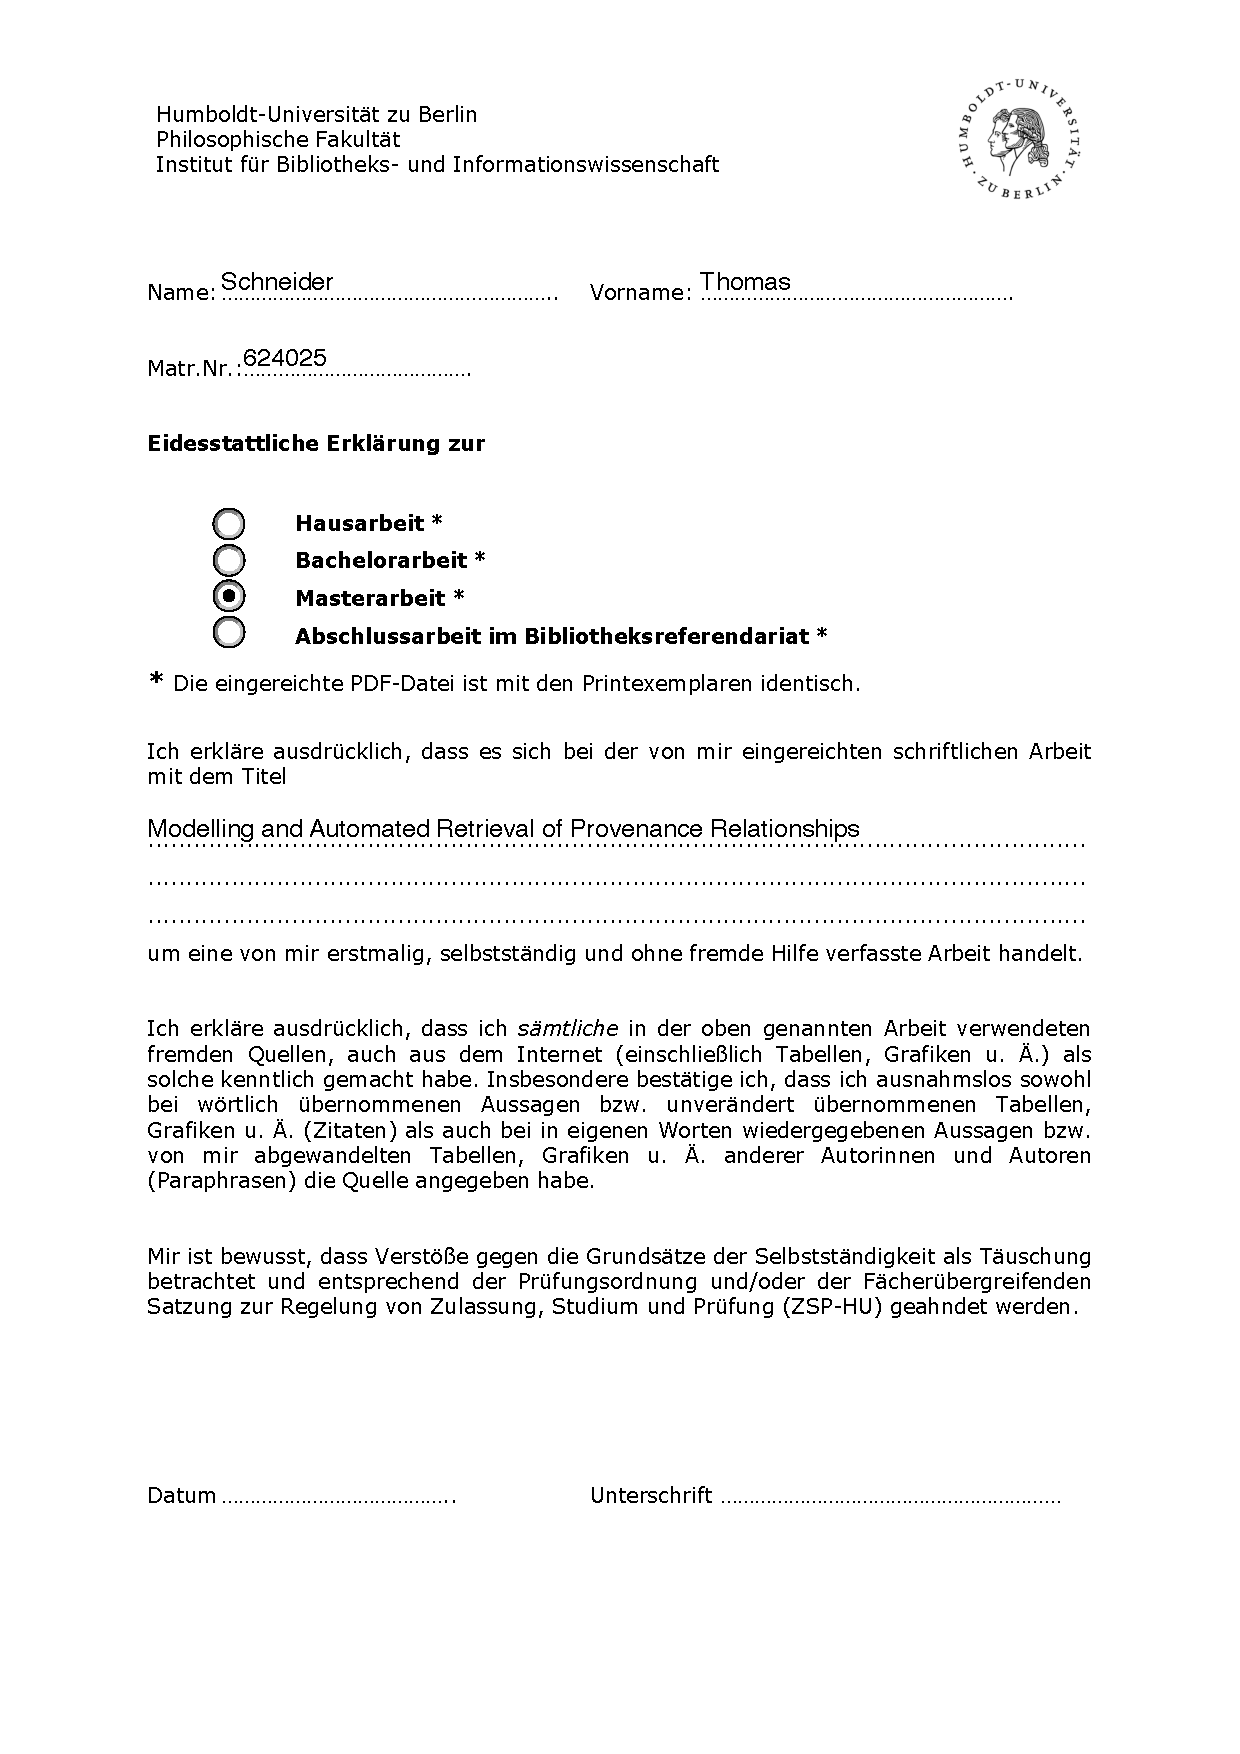
\includepdf[%
    addtotoc={1,chapter,0,Selbstständigkeitserklärung,selbststaendigkeitserklaerung},
    pagecommand={\thispagestyle{empty}\signature}%
  ]{%
    img/Selbststaendigkeitserklaerung_TS_printed.pdf%
  }
  
%  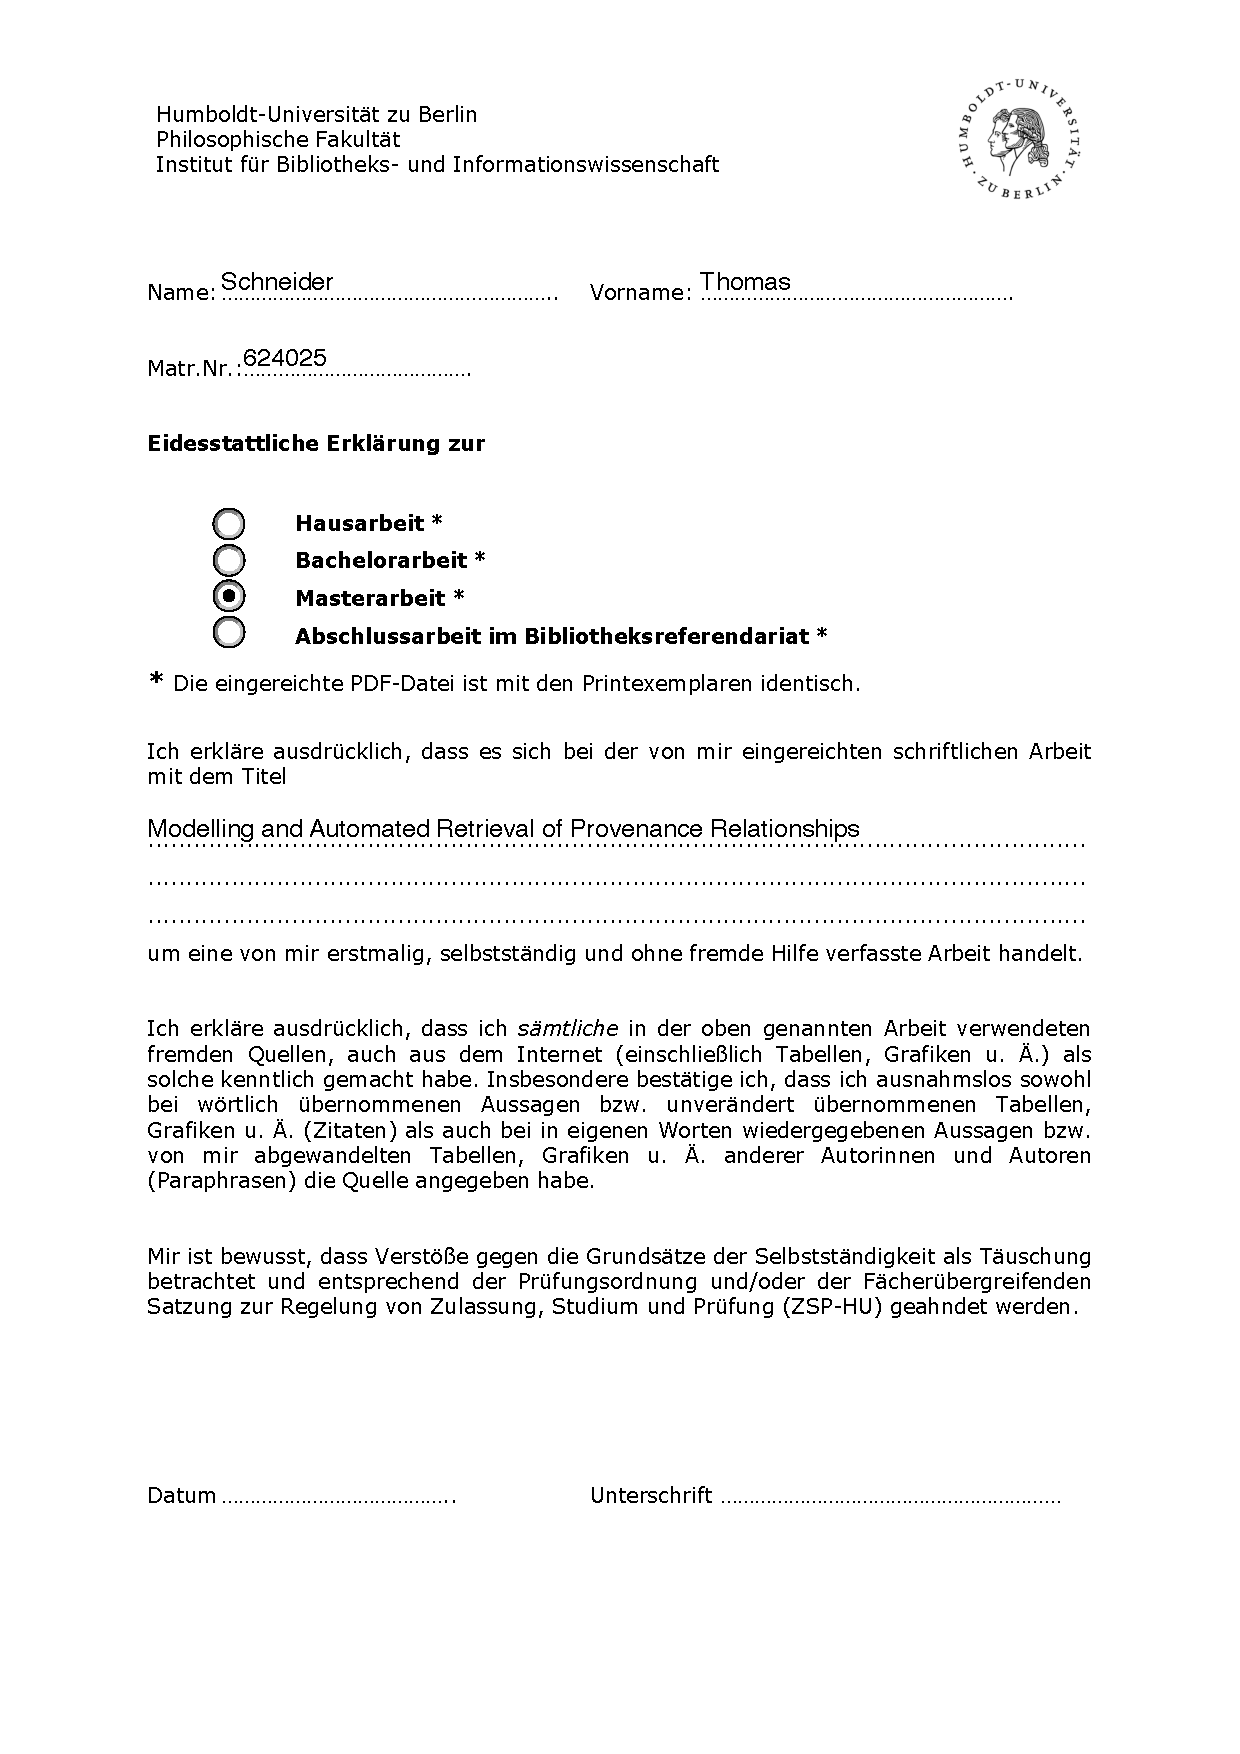
\includepdf[addtotoc={1,chapter,0,Selbstständigkeitserklärung,selbststaendigkeitserklaerung},pagecommand={}]{img/Selbststaendigkeitserklaerung_TS_printed.pdf}


\end{document}
